\documentclass[type=msc,colorback,accentcolor=tud1d,bigchapter]{tudthesis}
\usepackage[english]{babel}
\usepackage{graphicx}
\graphicspath{ {images/} }
\usepackage{comment}
\usepackage{csquotes}
\usepackage{hyperref}
\usepackage{listings}
\usepackage[plain]{fancyref}
\usepackage{pgfplots}
\usepackage{textcomp}

\usepackage[backend=biber,isbn=false,doi=false,style=ieee,maxbibnames=99,maxcitenames=99]{biblatex}
\usepackage[font=small,skip=10pt]{caption}

\addbibresource{references.bib}
\newcommand{\shellcmd}[1]{\texttt{\footnotesize\# #1}}
\graphicspath{ {images/} }
%\setinstitutionlogo{logo.eps}
\newcommand{\getmydate}{%
  \ifcase\month%
    \or Januar\or Februar\or M\"arz%
    \or April\or Mai\or Juni\or Juli%
    \or August\or September\or Oktober%
    \or November\or Dezember%
  \fi\ \number\year%
}

\newcommand*{\fancyreflstlabelprefix}{lst}
\fancyrefaddcaptions{english}{
  \providecommand*{\freflstname}{listing}
  \providecommand*{\Freflstname}{Listing}
}
\frefformat{plain}{\fancyreflstlabelprefix}{\freflstname\fancyrefdefaultspacing#1}
\Frefformat{plain}{\fancyreflstlabelprefix}{\Freflstname\fancyrefdefaultspacing#1}

\lstset{
  basicstyle=\fontsize{9.2pt}{9.6pt}\ttfamily,
  backgroundcolor=,
  keywordstyle=\bfseries\color{blue},
  keywordstyle=[2]\bfseries\itshape,
  commentstyle=\color{gray},
  stringstyle=\color{black},
  numberstyle=\scriptsize,
  breakatwhitespace=false,
  breaklines=true,
  prebreak = \raisebox{0ex}[0ex][0ex]{\ensuremath{\hookleftarrow}},
  escapeinside={@}{@},
  frame=lines,
  keepspaces=true,
  numbers=left,
  numbersep=4pt,
  rulecolor=\color{black},
  showspaces=false,
  showstringspaces=false,
  showtabs=false,
  stepnumber=1,
  tabsize=2,
  columns=fullflexible
	}
  % linewidth=.9\textwidth,

%\newcommand{\quotes}[1]{``#1''}
%\listoffigures
%\listoftables

\begin{document}
  \thesistitle{A distributed 3D Print Driver}%
    {}
  \author{Suman Bidarahalli}
  \birthplace{India}
  \referee []{Prof. Dr. Arjan Kuijper  }|{Ph. D. Alan Brunton }
  \department{Fachbereich Informatik}
  \group{Graphisch-Interaktive Systeme}
  
  \dateofexam{\today}{\today}
 % \tuprints{12345}{1234}
  \makethesistitle

\abstract
Determining material arrangements to control high-resolution multi-material 3D printers for reproducing shape and visual attributes of a 3D model (e.g. spatially-varying color, translucency and gloss) requires large computational effort. Today\textquotesingle s resolution and print tray sizes allow prints with more than \begin{math}10^{12}  \end{math} voxels each filled with one of the available printing materials (today up to 7 materials can be combined in a single print). Cuttlefish, a 3D printing pipeline, processes the input in a serial fashion leading to increased computation time for higher number of models. Distributed computing is one way of achieving better performance for large computations. Through this master thesis, we have developed a distributed version of the cuttlefish printer driver in which the computational task is distributed amongst multiple nodes in the cluster and the resulting partial output is merged to generate the full slices. The architecture supports streaming, which is required to rapidly start the print before the full computation is finished, as cuttlefish processes the input in small parts and generates chunk-wise output. Finally, the comparison of the performance achieved by the distributed vs the non-distributed cuttlefish version is established to get a better understanding of the advantages and the challenges of distributed computing.\newpage
	
\tableofcontents
\newpage
\listoffigures
\newpage
\lstlistoflistings
\newpage
\listoftables
\newpage
	
\chapter{Chapter}
\section{Introduction}
Additive manufacturing (AM) is a generic term used to describe the technologies that fabricate 3d Objects directly from 3D model data \cite{KRUTH}. ASTM International defines Additive Manufacturing as the process of joining materials to make objects from 3D model data, usually layer upon layer, as opposed to subtractive manufacturing methodologies \cite{cwig} . 3D Printing is one of the technologies encompassed by AM \cite{Conner}.3D Printing is a manufacturing method  wherein materials like plastic, polymer or metal, are deposited on one another in layers to produce a three dimensional object \cite{sdl}.  The prices of the materials used and the cost of the machinery involved in AM is dropping rapidly as well as the better engineered materials allow for high quality builds leading to the application of this technology in various fields. 

\section{3D Printing Process}

3D Printing is a 3-step process (Figure \ref{fig:3DP}) which includes creating a virtual design of the object (either by using designing software or through 3d scanners), slicing the 3d model before it can be printed followed by printing the object, and final step is the finishing process in which the printed object is cleaned up, polished or sanded, painted to complete it as intended.  
\begin{figure}[ht!]
\centering
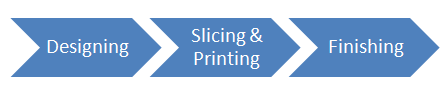
\includegraphics[scale=0.7]{3DPProcess.PNG}
\caption{3-Step 3D Printing Process}
\label{fig:3DP}
\end{figure}

The material chosen to print the object determines the underlying technology for the actual printing process, to name a few, if the material chosen is plastic then Fused Deposition Modeling (FDM) technology is used, for photo sensitive resin material the technology named Photo-polymerization is used, whereas SLS (Selective Laser Sintering) is the technology used if print material is powder (Alumide). Photo-polymerization is a technique that involves the use of UV light to solidify the photosensitive material.  This technique is used by different 3d printing processes like Stereo-lithography (SLA), Digital Light Processing (DLP) and MultiJet printers.  MultiJet printers begin by spraying the tiny droplets of photopolymer in the shape of the first layer followed by cross-linking the polymer by using the UV light from the lamp attached to the print head thus locking the shape of the layer in place \cite{dpW}. Multi-material printers enable fabrication of 3D prints which are composed of diverse materials i.e. materials which are fused to form the object may differ in their chemical properties, and/or physical properties \cite{Doubrovski}.\newline

The step 2 of the 3d Printing process involves the use of a software which enables conversion of the input (i.e. virtual design) to a form which is understood by the print machine. The software fundamentally performs couple of actions enlisted below before the data is sent to the printer:
\begin{itemize}
\item Parses the input and converts it to an internal representation
\item Performs slicing using the internal representation - Slicing is the procedure of dividing the 3D model into 2D layers where in each layer is a \textsl{slice}- a per print layer 2D representation of printer parameters for each (x,y) coordinate. Slicing can be thought of as similar to integrals i.e the 3D object can be approximated by it's derivatives i.e. 2D slices.[see Figure \ref{fig:slicing} \cite{slicing}]
\begin{figure}[ht!]
\centering
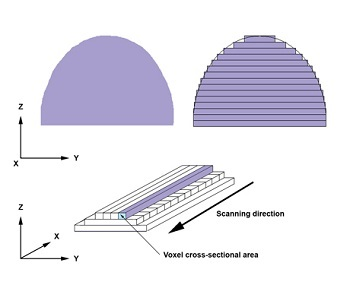
\includegraphics[scale=0.6]{slicing.PNG}
\caption{Slicing}
\label{fig:slicing}
\end{figure}

\item Assign materials to the 2D-Slices. 
\item Convert the 2D slices into machine specific code or representation.
\end{itemize}

The last step of 3D Printing is finishing up the printed object. The importance of this step should not be underestimated as it is worth the enormous effort to make the prints/prototypes look like objects made from real world materials (See Figure\ref{fig:Finishing}). The finishing techniques for the 3D printed objects can be referred as the craftsman's workshop, where patience, skills and experience can help transform the raw products of the printers into fully realized models. Majorly, finishing the prints involves sealing, polishing and painting which helps to bring out the smooth surface and fine feature details. For example, production grade plastic is used by FDM technology to print models which can be sanded, drilled or glued just like any another plastic part. 

\begin{figure}[ht!]
\centering
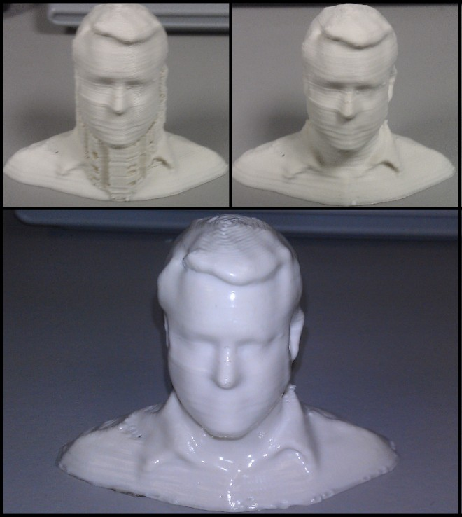
\includegraphics[scale=0.6]{Finishing.png}
\caption{Finishing}
\label{fig:Finishing}
\end{figure}


\section{Problem Statement}

Cuttlefish is a powerful print driver, which performs the transformation of the digital geometric representation of the design into machine-specific code or representation that eventually drives the 3D printer. Cuttlefish supports high-resolution multi-material printers and allows printing large sized multiple objects \cite{cuttlefish}. High-resolution multi-material prints consists of huge amount of voxels(easily up to \begin{math}10^{12}\end{math} as today \textquotesingle s printers allow to combine 7 materials in a single print),a voxel is 3D equivalent of 2D pixel \cite{3DString}. To reproduce the shape and attributes of the 3d model with high precision, Cuttlefish performs material assignment at voxel level. To do so large amount of computational effort is needed which cannot be achieved efficiently by a single processing entity for higher number of objects.  Moreover, cuttlefish processes the input in serial fashion leading to increased amount of computational time for multiple objects. \newline

To achieve a reasonable performance for large computations, distributed computing can be used \cite{DistComp} \cite{Desai}.  Distributed computing is concept where in multiple machines of a distributed system work together on a single problem domain \cite{rouse}.  A distributed system can be defined as the group or cluster of autonomous computers which are connected via network and communicate primarily through message passing \cite{coulouris}. The ultimate goal of distributed computing is to maximize performance by enhancing resource utilization in a cost effective, transparent and reliable manner.\newline

The state of the art multi-jet 3D printers allow printing high resolution large sized multiple print objects at the same time. To efficiently exploit the offered functionality of these printers, appropriate digital fabrication software needs to be developed. Through this master thesis, I have implemented a distributed version of cuttlefish 3dPrinting pipeline by applying the various concepts of distributed computing. The pre-processing task of the large sized multiple objects can be distributed among the nodes of the distributed system so as to utilize the processing power of each node in order to increase the efficiency by limiting the computational effort and time for each node.   Distribution of the tasks among the nodes of the distributed system parallelizes the pre-processing of the input thereby reducing the waiting time for each object to be processed. 
\newpage
  
\chapter{Related Work}

With science and technology progressing rapidly, there is a good chance of availability of already implemented solution for a given problem identified in a target system. This chapter highlights the existing systems in place which provide solutions designed to achieve similar goals to the thesis under discussion and comparison to how the solution presented in the current document differs from them. This chapter is divided into two sections with the first section briefly describes the existing distributed systems which can be used for cluster computing followed by the second section focusing the use of distributed systems in the field of 3D printing.

\section{Introduction to distributed systems and its types}
A distributed system consists of autonomous systems (AS) connected through network which interact (if necessary) through message passing and most importantly give the user an illusion of being single large system \cite{DCE}. The main goal of distributed system is to connect the users and the available infrastructure i.e. IT resources, in a transparent, open, cost-effective, reliable, scalable way. Transparency in distributed computing environment (DCE) means that the user is unaware of the underlying system complexities in terms of location of the AS, heterogeneity of the system hardware, concurrency and replication of the AS mainly to provide reliability and fault tolerance. Transparency property of the distributed systems makes it appear as a single system dedicated to perform some tasks to the user \cite{DSBook}. Scalability refers to the property by which the number of AS in the DCE can be increased (scaled in) or decreased (scaled out) so as to provide best suited infrastructure to handle the fluctuating load (i.e. the amount of work to be done). The shared resources of the distributed system can be broadly classified as physical resources and virtual resources. The Figure\ref{fig:TypesOfResourceSharing} details the resources included in the two categorizes. 

\begin{figure}[ht!]
\centering
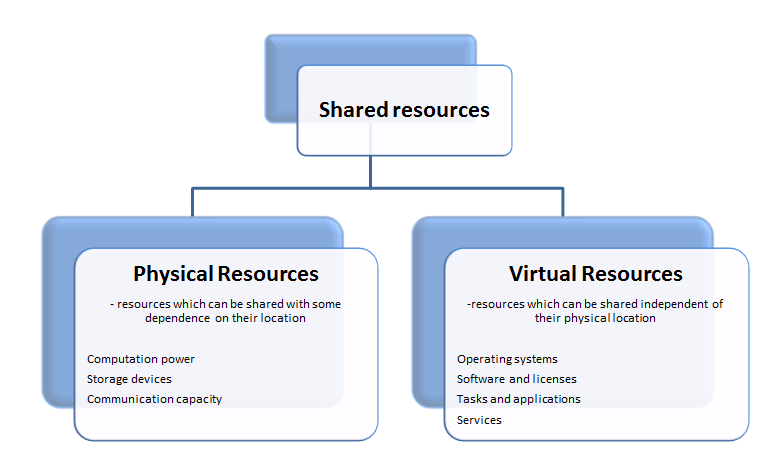
\includegraphics[scale=0.6]{TypesOfResourceSharing.PNG}
\caption{Distributed System Shared Resource Classification}
\label{fig:TypesOfResourceSharing}
\end{figure}
  
Distributed Computing is a vast domain which consists of various different types of computing environments like utility computing (grid computing and cloud computing), cluster computing, and peer-to-peer computing (Figure \ref{fig:DistributedComputingEnv}) which are described briefly as follows.

\begin{figure}[ht!]
\centering
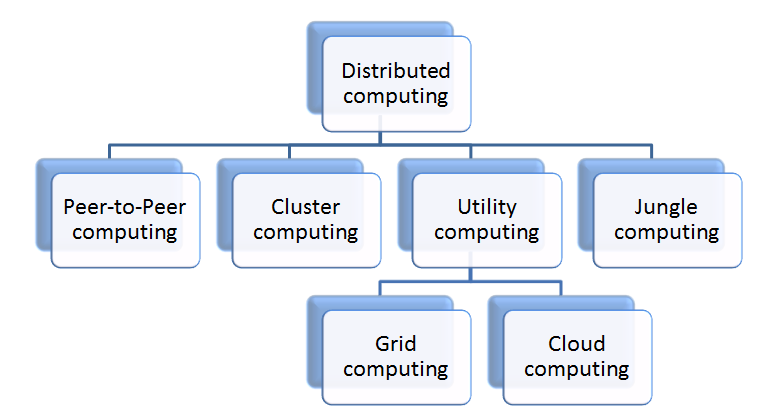
\includegraphics[scale=0.6]{DistributedComputingEnv.PNG}
\caption{Distributed Computing Environment}
\label{fig:DistributedComputingEnv}
\end{figure}

\begin{itemize}
\item \textbf{Peer-to-Peer computing}- Each node in the DCE acts as both client and server, providing as well as consuming part of the system resources. Peers are machines simply connected to the internet where in each peer can freely join and leave the DCE without affecting the whole system making the system self-organizing  and also implying no particular role (either master or slave) for a peer (Figure \ref{fig:P2P}).

\begin{figure}[ht!]
\centering
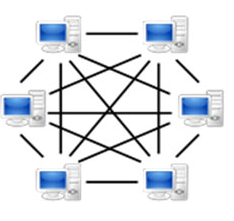
\includegraphics[scale=0.6]{P2P.PNG}
\caption{Peer-to-Peer system}
\label{fig:P2P}
\end{figure}

\item \textbf{Utility computing}- Utility computing is based on a model for service provisioning, which allows the users (consumers) to pay the providers for using the service only when they need to. It emphasizes on a business model, by which service providers make available the requested/paid resources to the costumers. All grid/cloud platforms are regarded as utility service providers. Grid computing enables coordinated resource sharing and problem solving in dynamic, multi-institutional virtual organizations where as cloud computing is a computing paradigm that involves outsourcing of computing resources with the capabilities of  replaceable resources and scalability i.e on-demand provisioning with little or no up-front IT infrastructure investment costs. Cloud computing offers its benefits through three types of delivery models namely- infrastructure-as-a-service (IaaS), platform-as-a-service(PaaS) and software-as-a-Service (SaaS) 

\item \textbf{Cluster Computing}- A cluster is a set of stand-alone computers and a network interconnecting them. The computers of the cluster work cooperatively together as a single integrated computing resource. A cluster is local if all of its component subsystems are supervised within a single administrative domain, usually residing in a single room and managed as a single computer system. The components of a cluster are connected to each other through fast local area networks. 

As mentioned in the brief description of different distributed systems, each node is similar to the other in a peer-to-peer system and it can join/leave the distributed system without affecting the user. As the requirement of the thesis design needed designated roles for the nodes, a peer to peer system does not fulfill the requirement of specific node roles in distributed system. A Peer-to-Peer system mostly uses internet to maintain connectivity amongst the peers. The distributed system to be used in the thesis has nodes which were connected through the enterprise network and it was not possible for a node outside the institution to join the system, which makes peer to peer system not an ideal choice. Grid computing essentially has systems which are offered by multiple institutions as resources, which dedicated to perform part of computation required for solving huge problems. The institutions which offer their systems form a virtual organization and only these institutions have shared access rights on the resources \cite{DSBook}. The distributed system in demand for the thesis is dedicated to be used for a specific enterprise and other institutions not part of the same network cannot contribute computes nodes. This makes grid computing not suitable as a distributed system for the thesis under discussion. 


\subsection{Use of Distributed Computing in fields involving large computations}

Distributed systems offer various advantages like computational speed-up, robustness through duplication of the resources, cheaper and scalable infrastructure etc. 
Using distributed systems allows to overcome the limitation of resources for solving problems with large computation, making it possible to get correct results within in a shorter span of time. The various domains where distributed computing has been used involves astronomy: for example Cosmology@Home is a project started to design models which describe the universe \cite{coshome}, data analysis and machine learning: the DistributedDataMining project involved data analysis for stock market prediction and analysis of medical information \cite{DisDataMin}, molecular biology: RNA world distributed system uses bio-informatics software to study the structure of RNA \cite{rnaworld}, climate study projects started in Oxford University use distributed system to study the climate changes which help to draw models for more accurate climate predictions \cite{ClimaProj}, etc. \newline

  


\section{Existing solutions for 3D Printing}

As described in the Introduction, 3D Printing is one of the upcoming additive manufacturing process and a favorite research topic. There are various solutions available in the market for varying kinds of requirements in terms of material, appearances, cost etc. Out of the many interesting solutions available, there are three solutions which are most relevant with respect to the current thesis topic as they use distributed system as an integral part of their solution. {\lq}\textbf{3dPrinterOS}{\rq} is a cloud-based management software for 3D printers which provides tools for making 3D printing user-friendly \cite{3dprinteros}. The user can connect the local 3D printer to the internet using the software provided by 3DPrinterOS thereby allowing the cloud-based software to drive the connected printer. It allows three input file formats (obj, amf and STL). The management software provides a tool to perform orientation of the print object on the print bed and to scale the size of the object as well as the slicer to perform slicing by allowing the user to set the slice thickness. The 3dPrinterOS software can be used only for the printers which are supported by it and does not act as a universal printer driver. The software allows to drive the connected printer but does not provide a way to generate output which can be then used to control the printer i.e. in our case bitmaps or STL output. During installation of the software to connect the local printer to the cloud, there are numerous device drivers which are installed on the client machine which might not always be ideal as there could be various trust issues associated with installation unknown device drivers from random sources. \newline

{\lq}\textbf{3DHubs}{\rq} is an online services which allows the user to provide digital input of the print object, select the material to be used to print the input and last but not the least select the print lab (where the object is printed locally and shipped to the user) by comparing the prices for printing the object \cite{3dhub}. It is a commercial solution to enable 3D Printing as a service where in the user does not need to own a 3D printer. It provides easy access to different kinds of material as well as helps to avoid setting up the required infrastructure to make use of the 3D Printing technology. It is quite beneficial and cheaper for users who do not print quite often but might not be an ideal solution for frequently printing customers. To use the solution the 3d model is uploaded to the server, which might not be desirable for companies where the design needs to be highly-protected. Also, there are no additional tools to provide dimensions if the digital input needs to be scaled up or down. \newline     

The {\lq}\textbf{Collaborative Cloud Printing Service}{\rq} is a cloud-based service for utilization of the 3D Printing resource developed by Institute of Computer-aided Product Development Systems at University of Stuttgart \cite{Baumann2016}. The solution provided is within the academic context and not a commercial solution. The focus of the project was to facilitate sharing of 3D Printing resources, provide platform for developing or extending and testing BPMS (Business Process Management Systems). The underlying distributed system used is the internet where as the approach in the current thesis is to use the enterprise network and computers within the network as distributed system which would be more desirable for companies who have privacy of their print models as the primary concern. The output for the cloud service under discussion is a printed object where as for the distributed cuttlefish the output is not necessarily a 3D printed object.  


\newpage
	
\chapter{System Model}
Cuttlefish, as mentioned earlier, is a 3D printing pipeline, which processes one or more 3D digital models and outputs control code to drive a particular 3D Printer to realize the the object. The digital model of the object to be printed is created either using a modeling software or acquired by 3D scanners. Cuttlefish allows  numerous input file formats like STL, OBJ, PLY, WRL. 

The whole pipeline has a streaming architecture, which means that the input can processed in smaller parts so as to generate the output sooner thus letting the printing process to be started as early as possible i.e. even before the whole object has been processed.The output is generated in parts called as \textit{chunks}- each chunk is a collection of 2D layers, where each layer is referred to as a \textit{slice}. \newline

\section{Non-distributed Cuttlefish Pipeline Components}

The pipeline also has a component-based architecture. The composition of the pipeline varies as per the components assembled to form the pipeline. The components of the pipeline can be chosen on the basis of factors like the type of generated output needed to drive the particular printer, for example \textit{Bitmaproducer} component if the desired output is bitmaps, where as \textit{STLProducerObjet} component is included when the desired output is an STL file per print material, i.e. a mesh representation, or if the output required is a GCode then the component used is \textit{GCodeProducer}, e.g. for FDM printers. Another factor for deciding the components of the pipeline is what attributes of the object should be reproduced: shape, color, translucency, internal structure, etc
\newline

The pipeline performs the following fundamental steps in a serial fashion irrespective of the components forming the pipeline \ref{fig:TypicalCuttlefishSteps}. Let us now examine each of the stages outlined in Figure 3.1:

\begin{figure}[ht!]
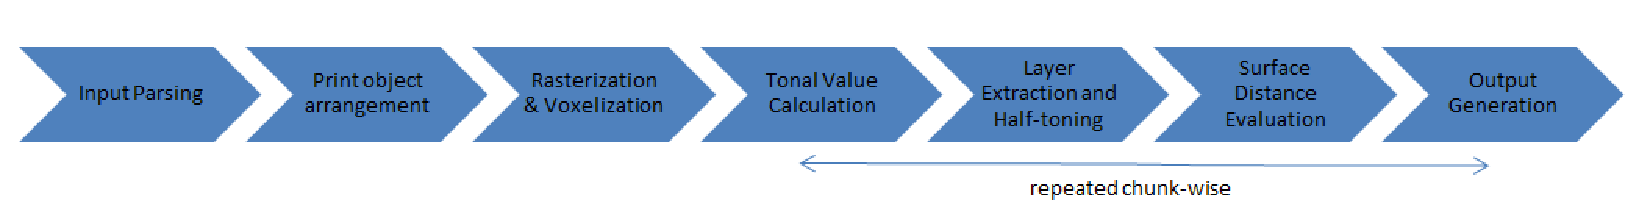
\includegraphics[scale=0.6]{TypicalCuttlefishSteps.pdf}
\caption{Cuttlefish pipeline component functionality}
\label{fig:TypicalCuttlefishSteps}
\end{figure}

\begin{itemize}
\item \textbf{Input Parsing}: The input given to the pipeline, mostly mesh files and textures, is parsed and internal mesh representations are created for them. Internal mesh representations of multiple objects can be grouped into print jobs, together with each having it\textquotesingle s own unique identifier and is referred to as a print object. At present \textit{FileParsePj} is the component which performs this task. \newline 

\item \textbf{Print object arrangement}: The print objects are arranged within the print volume to lower the material consumption and the print time. The arrangement of the print jobs is done by first optimizing the orientation of each print object to reduce print time and support requirements, followed by a greedy approach where in to arrange the print objects (approximated by their bounding boxes) compactly within the print volume. \textit{PrintJobOrganizer} is currently handling this task. \newline 

\item \textbf{Rasterization and Voxelization}: Rasterization is the process of converting vector graphics, e.g. polygons or curves, to raster images,i.e. pixels or dots for output to printer or display device. In our context, the input surface representation is converted to a \textit{voxel} representation-\textit{a voxel is 3D equivalent of 2D pixel}, and each voxel intersecting the surface is assigned attributes like color, occupancy etc. Currently the component doing this is \textit{PrintJobVoxelizer}. The algorithm used for voxelization can be varied using the component configuration and further details are beyond the scope of the thesis. \newline 
 
\item \textbf{Tonal Value Calculation}: This step involves calculation and assignment of tonal values from the optical features (RGB or BRDF data) of surface voxels. The tonal value computation is done with the help of a calculated ICC-profile  belonging to the specific printer. The component doing this is referred to as \textit{TonalValueCalculator}.

\item \textbf{Surface Distance Evaluation and Tonal Analyzer} (optional): The component evaluates the distance of voxels to the surface and assigns values of a given attribute (of the surface voxel)  to inner voxels within the specified maximum distance.The Tonal value analyzer component reports summary statistics, comparing the half-toned signal to the original tonal values in easy to interpret graphs.\newline

\item \textbf{Layer Extraction and Half-toning}: The component \textit{LayerExtractor} extracts the layers below surface which are subsequently half-toned by the component LayerHalftoner. Half-toning is the process of creating an image comprised of discrete dots rather than continuous tones.When viewed from a distance, the dots blur together, creating the illusion of continuous tones. Details can be found in \cite{Brunton}. \newline

\item \textbf{Output Generation}: The generated slices are then used to create the desired output, e.g bitmaps or STL files. The output files are then used to drive the print machine. \newline

\end{itemize} 

The input given to the printer driver is a main configuration file in a \textit{JSON} format - \textit{JSON} (JavaScript Object Notation) is an open-standard format that uses human-readable text to transmit data objects consisting of attribute-value pairs, describing various input fields. The main configuration file lists the files describing the printer specification, component configuration, geometry, appearance, logger type and output folder path. The printer specification file consists of the details related to the resolution of the printer, print volume, material names and unique identifier for each material, \textit{ICC profile}- it is a file which contains data that characterizes any color input/output devices. The component configuration enlists the components forming the pipeline and configuration parameters for each component. Listing \ref{lst:CC} is an example of the \textit{BitmapProducerObjet} component configuration description. \newline

\begin{lstlisting}[label={lst:CC},caption={\textit{BitmapProducerObjet} Component Configuration}]
{
	"type":"BitmapProducerObjet",
  "OutputPath": "Output/",
  "PrinterTextFileName": "printer_config.txt",
  "computeType":"multi-threaded",
  "pitchRequirement": "32",
	"unusedMaterial":"VeroClear"
}
\end{lstlisting}

The \textit{type} field denotes the name of the component and \textit{computeType} sets the component to run in a single-threaded or multi-threaded fashion. \textit{OutputPath} is used to set the path at which the component generates the bitmaps and \textit{pitchRequirement} value is used to make the bitmap width a multiple of the specified number. The component which parses the input main configuration file creates a \textit{PrintingSoftware} for the given component configuration. 

\section{System Model for Distributed Cuttlefish Pipeline} \label{sysMod}

The non-distributed cuttlefish pipeline runs on a single machine and therefore there is no particular machine specific action needed to be performed depending on the role of the machine. For an application to run on a cluster of machines, sometimes it is necessary to perform additional steps which are specific to the role of the node in the cluster. Before understanding the architecture of the distributed cuttlefish printer driver it is necessary to understand the architecture of the cluster, referred to as a distributed system, on which the driver is designed to run. 

\subsection{Distributed system for cuttlefish printer driver} \label{clusterArch}

The distributed cuttlefish printer driver is developed using a cluster of the computers(nodes) which are heterogeneous in their hardware as well as software configuration and are connected via a standard workplace network. The initial set up used during the development had three nodes out of which one node is the master node and remaining nodes are the slave nodes. The names master and slave depict a predetermined role the nodes have and type of work they do. The nodes also have access to a shared networked file system (figure \ref{fig:CuttlefishCluster}).

\begin{figure}[ht!]
\centering
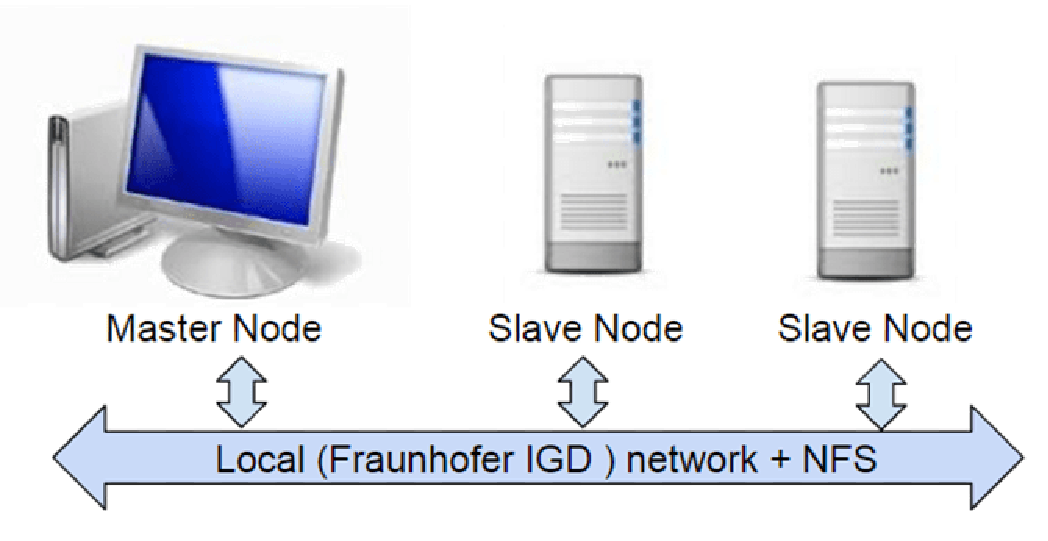
\includegraphics[scale=0.6]{CuttlefishCluster.pdf}
\caption{Cluster setup}
\label{fig:CuttlefishCluster}
\end{figure}

As mentioned earlier, the role of the node determines the type of work they do.The master node is the computer in the cluster where the user submits his request, namely the main configuration file (figure \ref{fig:Step1}). 

\begin{figure}[ht!]
\centering
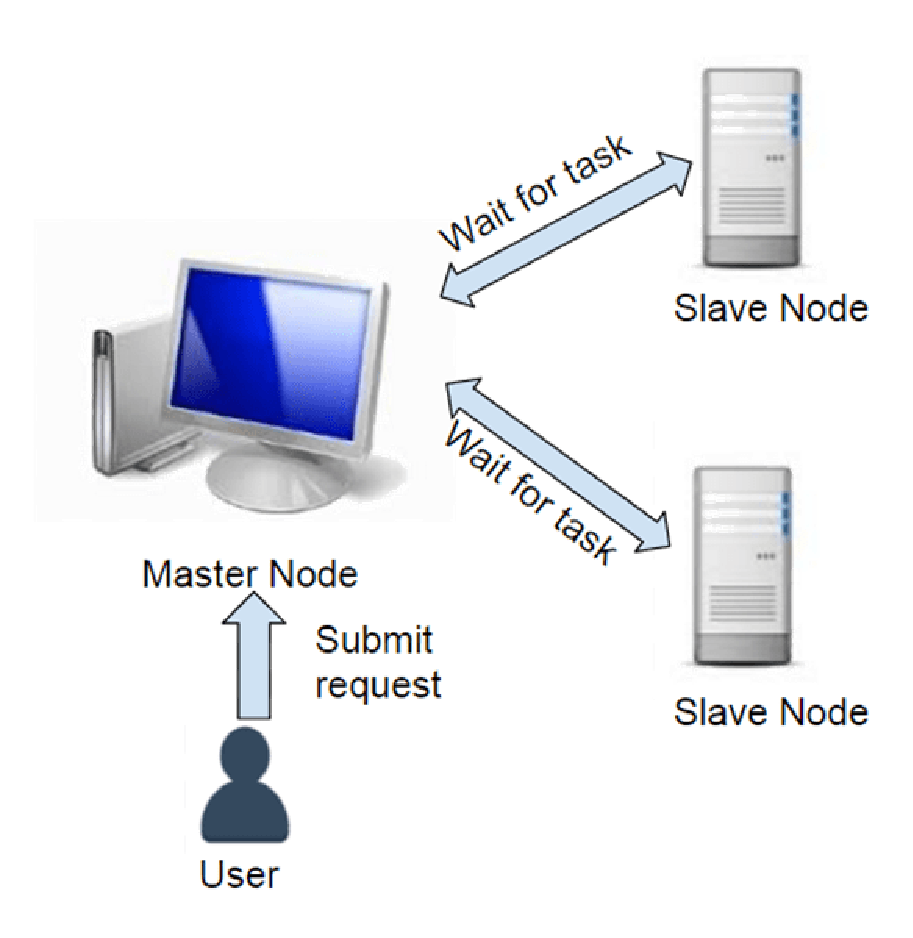
\includegraphics[scale=0.6]{Step1.pdf}
\caption{User submits the request}
\label{fig:Step1}
\end{figure}

The master node then performs some computation and distributes the sub-tasks to be performed by the slave nodes (figure \ref{fig:Step2}). 

\begin{figure}[ht!]
\centering
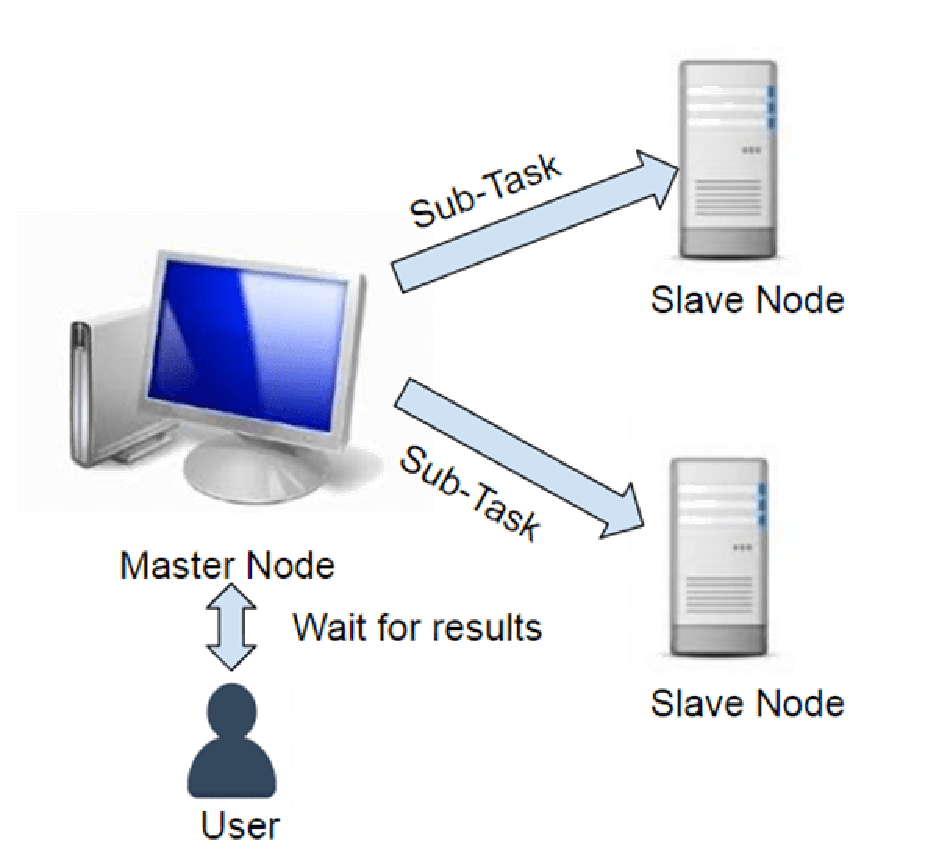
\includegraphics[scale=0.6]{Step2.pdf}
\caption{Master distributes the sub-tasks}
\label{fig:Step2}
\end{figure}

The slave nodes perform the assigned tasks and report back to the master (figure \ref{fig:Step3}). The cluster nodes follow a classic \textit{master-slave} communication paradigm. 

\begin{figure}[ht!]
\centering
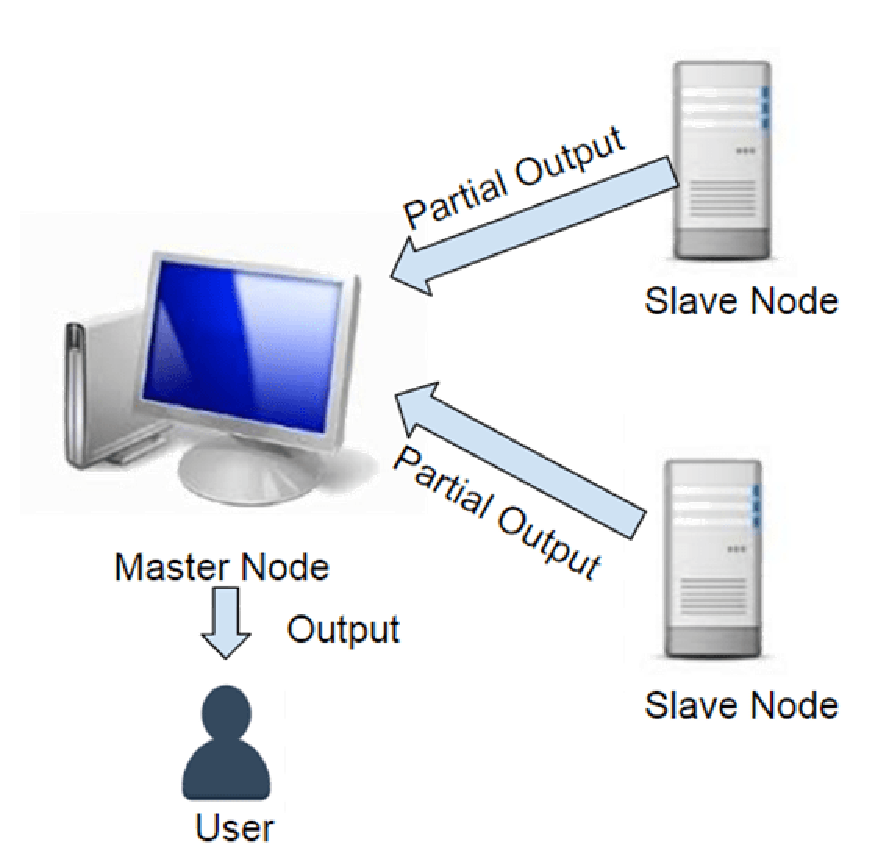
\includegraphics[scale=0.6]{Step3.pdf}
\caption{Slaves report the partial output}
\label{fig:Step3}
\end{figure}

\subsection{Components of distributed cuttlefish printer driver} \label{DSCuttlefish}

The distributed cuttlefish pipeline components may differ depending upon the role of the node in the cluster. The components put together form a printing software in which the components run on the node in a loop, with each iteration of the loop processing chunk-wise data. To apply distributed computing as a solution for stated problem of large computation on big data set, there are three additional steps, as enlisted below, some of which need to be performed either on the master or the slave node:  
\begin{enumerate}
\item Division of task into sub-tasks 
\item Awaiting the sub-tasks and doing the needed work
\item Submitting back the partial output
\end{enumerate}

\subsubsection{Master Node Printing Software Components}

\begin{figure}[t]
\centering
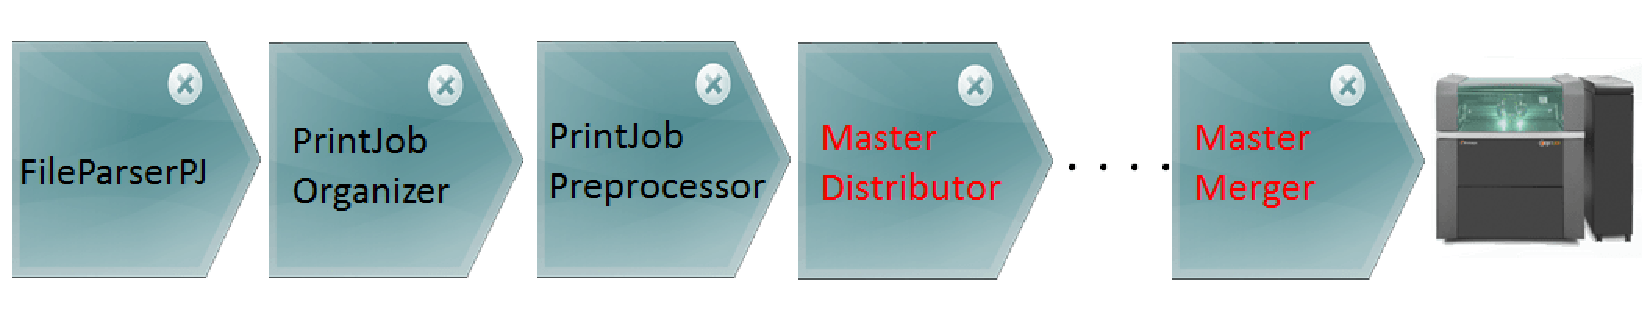
\includegraphics[scale=0.6]{MasterPSPl.pdf}
\caption{Master Node Printing Software Components For Prototype I}
\label{fig:MasterPS}
\end{figure}

As per the model discussed in the section \ref{clusterArch}, the master node performs the step $1$ from the above steps. The division of the task among the slave nodes needs to be performed by the master efficiently so as to make sure that distributed load is balanced and none of the slaves are over-worked. To do so, the master needs to evaluate the input and perform some measurements so as to make a wise decision regarding the task split. Hence, the master printing software needs to at least parse the input into an internal mesh representation i.e. print jobs and compute the necessary parameters on the basis of which an informed decision can be made. The component \textit{MasterDistributor} is responsible for division of the submitted task and takes the print jobs as input and generates sub-tasks as the output. After the successful generation of the sub-tasks, the distribution of the sub-tasks among the slaves is done. The form in which the tasks are distributed may vary leading to different designs of the component which is discussed in detail in the next chapter. 

\begin{figure}[t]
\centering
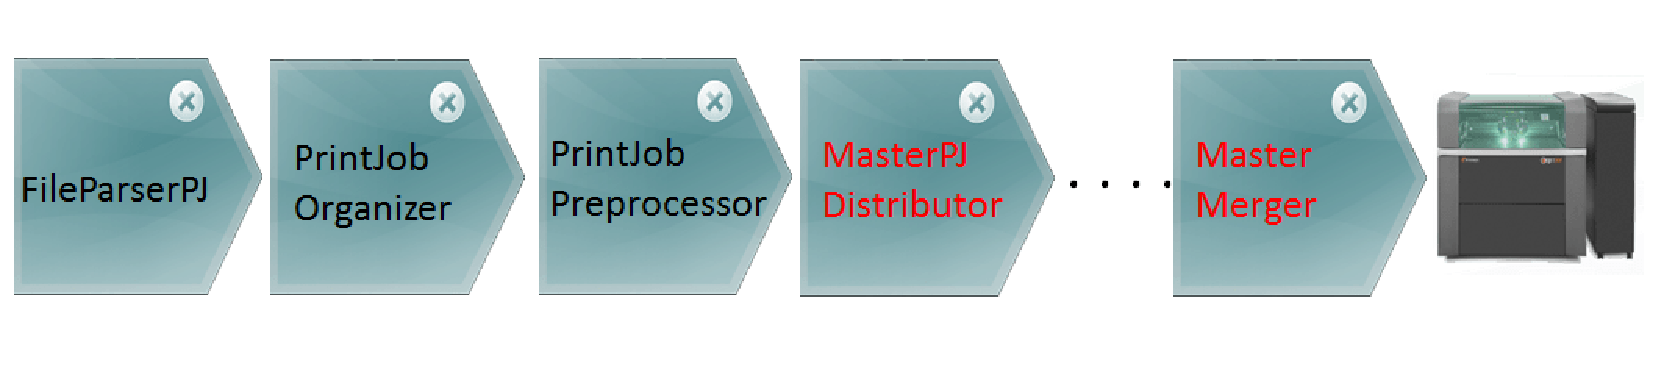
\includegraphics[scale=0.6]{MasterPSPIl.pdf}
\caption{Master Node Printing Software Components For Prototype II}
\label{fig:MasterPSII}
\end{figure}

On receiving the sub-tasks from the master, the slave nodes start doing their share of work. The master after submitting the sub-tasks has to wait for the slaves to generate the partial output. So as to maintain the streaming architecture, the slaves perform the assigned work in chunks and report the partial output to the master. The master then collects the partial output and performs some computation using received data and provides the final output to the user. \textit{MasterMerger} component in the master printing pipeline is responsible for receiving the partial output from all the slaves and combining it before sending it on to the output component. The output from the slave nodes are the chunks of partial \textit{slices} which are later merged into chunks of full slices. Figure \ref{fig:MasterPS} shows the components of the printing software running on the master node for Prototype I and Figure \ref{fig:MasterPSII} for prototype II .

\subsubsection{Slave Node Printing Software Components }

\begin{figure}[t]
\centering
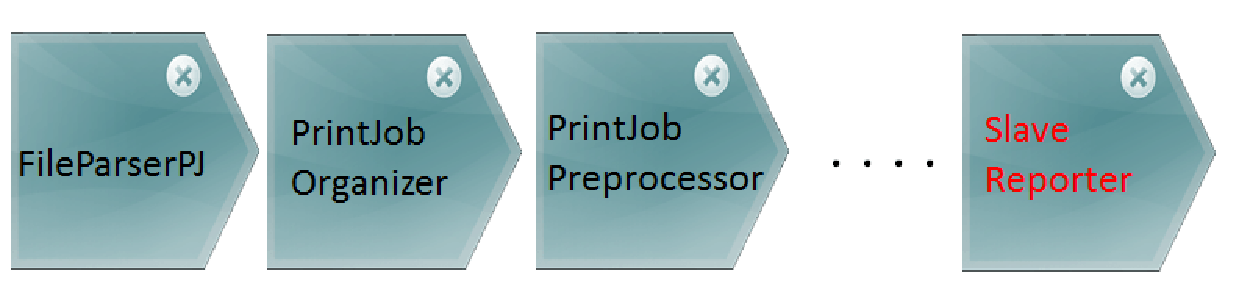
\includegraphics[scale=0.6]{SlavePSPI.pdf}
\caption{Slave Node Printing Software Components For Prototype I }
\label{fig:SlavePS}
\end{figure}

\begin{figure}[t]
\centering
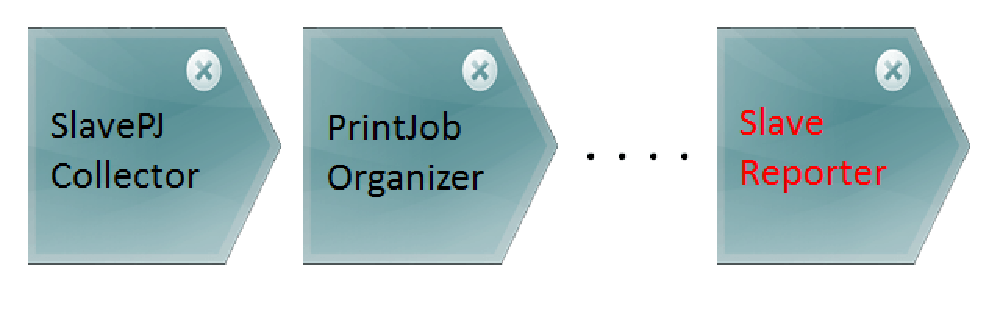
\includegraphics[scale=0.6]{SlavePSPII.pdf}
\caption{Slave Node Printing Software Components For Prototype II }
\label{fig:SlavePSII}
\end{figure}

The slave nodes in the cluster (i.e. all nodes other than the master are considered slave nodes) perform the assigned task and report back the results to the master node. To do so, the slaves nodes have to first wait until the master has divided the task submitted by the user into smaller sub-tasks. Once receiving the input, the slave nodes run the whole printing software (similar to the non-distributed cuttlefish version) with just one minor change. As the slave nodes report the partial output to the master, they do not need to run the output component, for example the \textit{Bitmapproducer}. The partial output which is reported by the slaves to master is in form of \textit{slices} and hence, the slave printing software running on the slave nodes does not contain the output component, instead it runs a component called the \textit{SlaveReporter} which, as the name suggests, reports the partial output in a chunk-wise fashion back to the master. Figure \ref{fig:SlavePS} shows the components of the printing software running on the slave node for Prototype I and Figure \ref{fig:SlavePSII} for Prototype II.

\clearpage

\newpage
		
\chapter{Design Analysis}
An algorithm can be defined as a set of precise (i.e., unambiguous) instructions that specify how to solve a given problem. An algorithm can be implemented in multiple ways leading to varying performance and efficiency of the program, for example, using different data structures, data storage options i.e. if the data should be stored in memory or on file system, implementation language, library functions used etc. A design is a result of such numerous decisions made with the goal to achieve a balance between efficiency and optimization. Very rarely is it possible to find the perfect design which would lead to a program performing with the same efficiency for the entire input space. Hence, while making the decisions it is important to evaluate the advantages and disadvantages of the chosen approach. This chapter is therefore dedicated to analyze the design choices made during the implementation. \\

As discussed in Section \ref{sysMod}, the task submitted by the user to the master node is divided into sub-tasks and distributed among the slave nodes of the cluster. The slave nodes perform the allocated work and report the partial output which is merged at the master node. The Figure \ref{lst:FC} summarizes the process. The \textit{MasterPrintingSoftware} follows the steps denoted in the left branch of the flow chart where as the \textit{SlavePrintingSoftware} follows the steps of denoted in the right branch of the flow chart. The \textit{MasterPrintingSoftware} and \textit{SlavePrintingSoftware} design decisions include:
\begin{enumerate}
\item Format of the sub-tasks allocated to the slaves nodes
\item Distribution of sub-tasks by the master
\item Format of the slave partial output 
\item Merging of the partial output 
\end{enumerate}

\begin{figure}
\centering
\begin{tikzpicture}[node distance=2.75cm] 
\node (start) [startstop] {Start};
\node (dec1) [decision,below of=start ,yshift=-0.75cm]{ Is master node?};
\node (Min1) [io, below left of=dec1 , xshift= -2cm] {Input main configuration file};
\node (Sin1) [io,below right of=dec1 , xshift= 2cm] {Receive sub-tasks from Master};
\node (Mpro1) [process, below of=Min1] {Parse Input, Create sub-tasks, Distribute Sub-tasks};
\node (Mpro2) [process, below of=Mpro1 ,yshift=-0.5cm] {Receive meta-data, compute full slice height, width, offset};
\node (Mpro3) [process, below of=Mpro2 ,yshift=-0.5cm] {Receive partial slices and merge to full slice};
\node (Mdec1) [decision,below of=Mpro3, yshift=-0.5cm]{ Is last slice?};
\node (Spro1) [process, below of=Sin1] {Perform application specific computation and generate chunk-wise slices };
\node (Sdec1) [decision,below of=Spro1, yshift=-0.5cm]{ Is first chunk?};
\node (Spro2) [process, below left of=Sdec1,xshift= -1cm] {Send meta-data to the master};
\node (Spro3) [process, below of=Sdec1,yshift=-1cm ] {Send the partial slice to the master};
\node (Sdec2) [decision,below of=Spro3, yshift=-0.5cm]{ Is last chunk?};
\node (Mend) [startstop,below of= Mdec1 , yshift=-1.5cm] {End};
\node (Send) [startstop,below of=Sdec2, yshift=-1.25cm ] {End};

\draw [arrow] (start) -- (dec1);
\draw [arrow] (dec1) -| node {yes}(Min1);
\draw [arrow] (dec1) -| node {no}(Sin1);
\draw [arrow] (Min1) -- (Mpro1);
\draw [arrow] (Mpro1) -- (Mpro2);
\draw [arrow] (Mpro2) -- (Mpro3);
\draw [arrow] (Mpro3) -- (Mdec1);
\draw [arrow] (Mdec1.west) -|node {no} ++(-0.5,0)|-(Mpro3.west);
\draw [arrow] (Mdec1) -- node {yes}(Mend);
\draw [arrow] (Sin1) -- (Spro1);
\draw [arrow] (Spro1) -- (Sdec1);
\draw [arrow] (Sdec1) -| node {yes}(Spro2);
\draw [arrow] (Sdec1) -- node {no}(Spro3);
\draw [arrow] (Spro2) -| (Spro3);
\draw [arrow] (Spro3) -- (Sdec2);
\draw [arrow] (Sdec2.east)-|node {no} ++(0.5,0)|-(Spro1.east);
\draw [arrow] (Sdec2) -- node {yes}(Send);
\end{tikzpicture}
\caption{Distributed Printer Driver Flow Chart}
\label{lst:FC}
\end{figure}

Each of the design possible from the various combinations of the above decisions yields a different behavior of the component responsible for that particular task. The following sections describes the two designs implemented through this thesis in detail.  

\section{Prototype I- Input/Output using Network File System } \label{protoI}

Prototype I is the base prototype wherein the nodes communicate amongst each other the input and the partial output using the shared network file system. The synchronization amongst the nodes is done via message passing. 

\subsection{Master sub-task creation and distribution}
The user submits the job to the master node using a configuration file in JSON format - \textbf{J}ava\textbf{S}cript \textbf{O}bject \textbf{N}otation is a syntax for storing and exchanging data. The JSON document contains a member called as \textit{PrintObjectFiles} whose member values indicate the geometry, texture, orientation etc of the object to be printed. The \textit{FileParserPJ} component of \textit{MasterPrintingSoftware} parses the set of input objects and converts it into set of print objects. Each print object contains a mesh representation of the geometry and the information related to it's appearance. The print objects are grouped together into a print job. Each print job is then organized in the print tray and then passed to the \textit{MasterDistributor} component which is in charge of sub-task creation and distribution. \\

The arrangement of the print objects on the print tray is done using a simple approach. For each print object the bounding box is calculated and the print object bounding boxes are sorted in the descending order i.e. largest to smallest. The whole print tray is seen as one big cell which contains the partitioned cells holding the print objects. For the first object i.e. is the one with the largest bounding box, the cell which fits the object is found and placed in the cell representing the print tray whose volume is equal to the print volume. The print volume is calculated by multiplying the height, width and length of the print tray. After placing the smaller cell, the larger print tray cell is split thus creating multiple smaller cells which can be chosen for the remaining objects. For each print object, the placement is recorded by the offset values of the cell in which it is placed starting from the origin. \\    

The sub-tasks distributed by the component can be already created print jobs or they can be in the same format as the received input i.e. configuration file. In this prototype, the \textit{MasterDistributor} creates a configuration file for each slave with the exactly same format as the configuration file parsed by the \textit{FileParserPJ} with a few changes i.e. the \textit{PrintObjectFiles} contains details of only the print models allocated to that particular slave and the \textit{OutputFolder} value is the folder location for the slave to write the partial output. In the Figure \ref{fig:MasterConfigurationFile}, the configuration file received by the master node has the \textit{PrintObjectFiles} containing four inputs models which are distributed by the master as seen in the Figure \ref{fig:Slave1ConfigurationFile} for the slave with rank 1 and Figure \ref{fig:Slave2ConfigurationFile} for slave with rank 2. 

\begin{figure}[ht!]
\centering
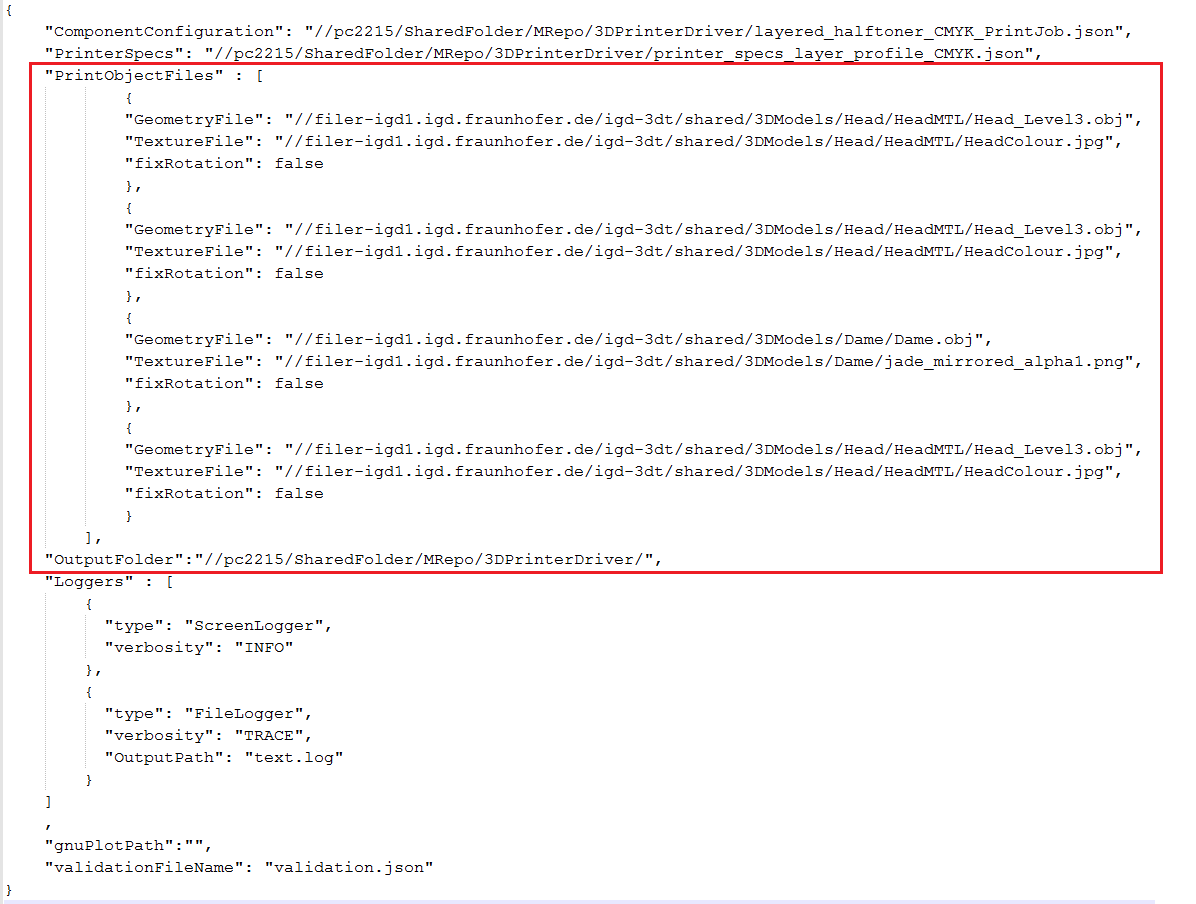
\includegraphics[scale=0.6]{MasterConfigurationFile.png}
\caption{Master Configuration file}
\label{fig:MasterConfigurationFile}
\end{figure}

\begin{figure}[ht!]
\centering
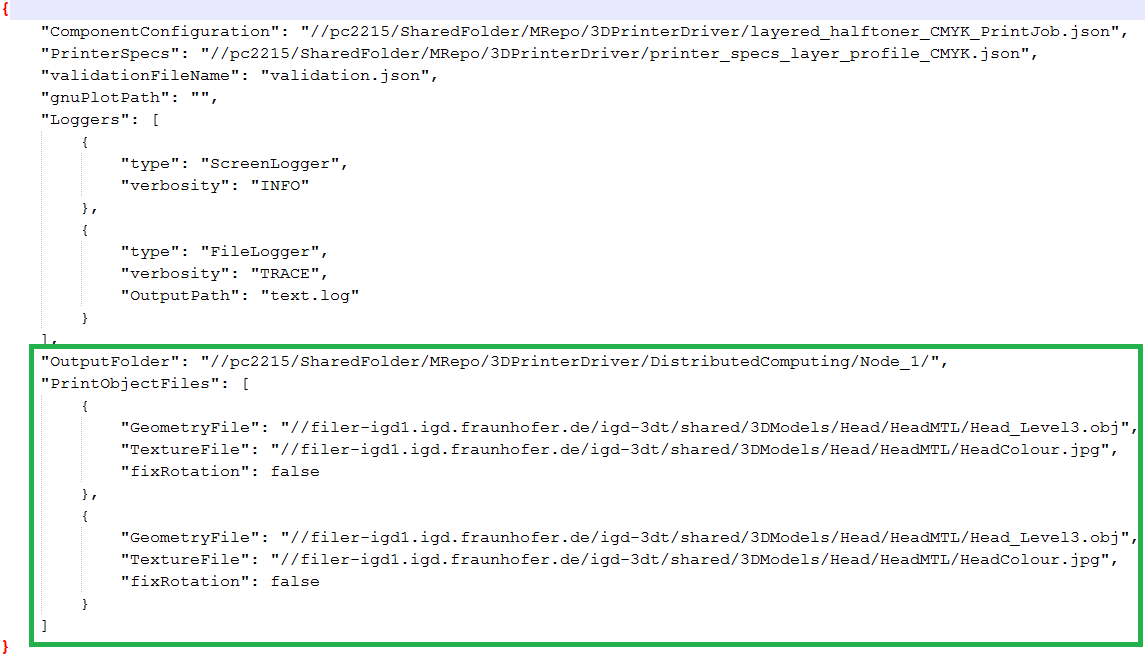
\includegraphics[scale=0.6]{Slave1ConfigurationFile.png}
\caption{Slave 1 Configuration file}
\label{fig:Slave1ConfigurationFile}
\end{figure}

\begin{figure}[ht!]
\centering
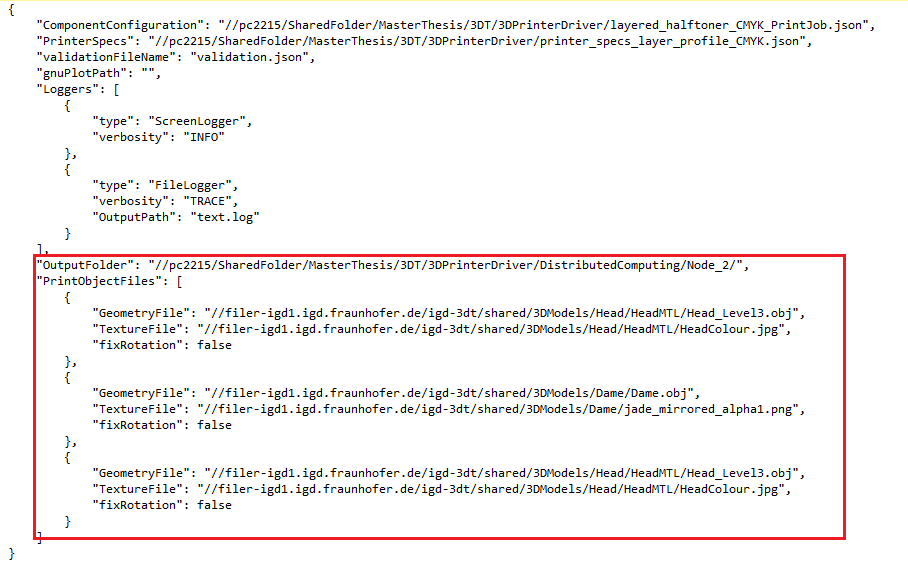
\includegraphics[scale=0.6]{Slave2ConfigurationFile.png}
\caption{Slave 2 Configuration file}
\label{fig:Slave2ConfigurationFile}
\end{figure}

This prototype is possible only if the cluster nodes have read/write permission to the shared network file system where the geometry, texture files and input/output folders are stored /created. The \textit{MasterDistributor} creates a unique path for each slave using the rank of the slave and writes the configuration file to this path. It then communicates to the slave only the path where the slave can find the configuration file. The sequence diagram in the Figure \ref{fig:SequenceDiagram1} summarizes the communication between the master and the slaves.  

\begin{figure}[ht!]
\centering
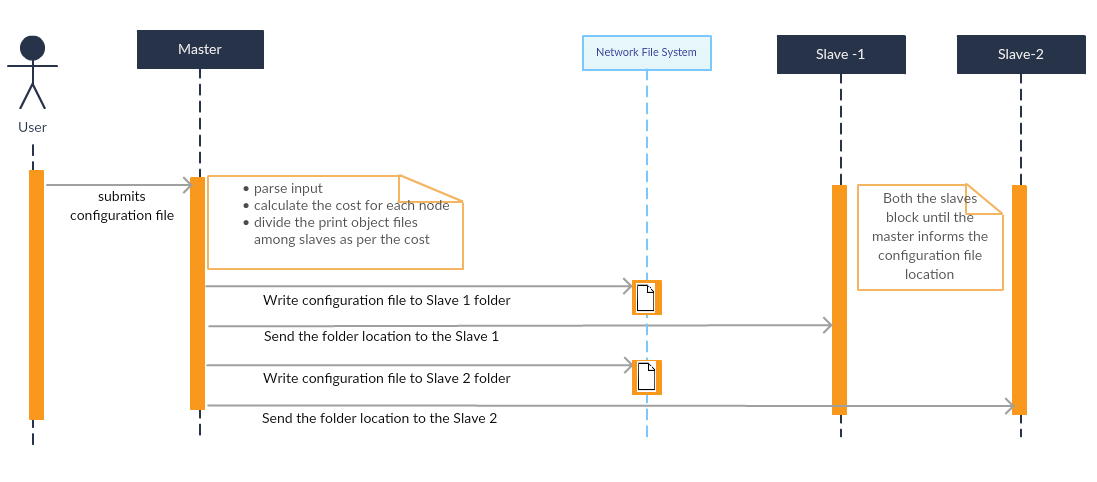
\includegraphics[scale=0.6]{SequenceDiagram1.png}
\caption{Master-slave input communication}
\label{fig:SequenceDiagram1}
\end{figure}

The advantages of distributing the sub-tasks through the configuration file are:
\begin{itemize}
\item \textbf{Design simplicity}: The most important aspect of this design is it's simplicity as the \textit{SlavePrintingSoftware} pipeline does not need to be modified greatly with respect to the serial 3D Printing pipeline, which means that it is almost similar to running a single instance of the non-distributed version of the 3D Printing pipeline. 
\item \textbf{Lower Communication Overhead}: Slave nodes are blocked until the master communicates the configuration file path to each slave. Communication of the file path is faster as it is less number of bytes to be exchanged among the nodes as compared to the number of bytes to be sent when print jobs are distributed .
\item \textbf{Faster Disk I/O}: The configuration file read and writes i.e. disk I/O (both at the master and slave) are much faster than sending the print job as series of bytes because of the additional steps (refer to section detailing the second prototype) that need to be performed while sending the print jobs. It is simpler implementation as communicating the print jobs as series of bytes would require serialization and deserialization of the print jobs with an additional effort of communicating the size along with texture information for each print object.
\item \textbf{No serialization and deserialization}: As the configuration files are in JSON format, there are very efficient library functions which allow to read and write the files with ease. As the format of the files is quite standard, there is no need for serialization and deserialization of the files even if the nodes have varying underlying system architecture.        
\end{itemize}

The disadvantages of distributing the sub-tasks via configuration file are: 
\begin{itemize}
\item \textbf{Dependency on shared network file system}: This prototype has a strong requirement that the nodes have a shared network file system and each node must have read access to the model texture/geometry file along with write access to the output folder to dump the partial output. If the print jobs are communicated as stream of bytes, it is possible to get rid of this requirement.
\item \textbf{Performance overhead}: The configuration file, model geometry and texture files are parsed twice, once by the master to create the prints jobs needed for cost computation and once by the slaves for actual computation. This leads to redundant execution of the \textit{FileParserPj} and \textit{PrintJobOrganizer} at both master and slave nodes which accumulates to a significant performance overhead (refer to the Section).
\item \textbf{Performance bottleneck at the master}: As the files are read and written to the shared network file system, the network bandwidth limits the speed of the disk I/O. With increase in number of slave nodes, the load at the master to write the configuration file per slave increases which may become a performance bottleneck. 
\end{itemize}

\subsubsection{Sub-Task Distribution}

The sub-tasks are distributed by the \textit{MasterDistributor} component based on a cost function. The goal of the distribution is to allocate equal work to each slave i.e. none of the slaves are over-worked and all of them finish the work almost at the same time. One of the main reasons which makes it important to achieve load balancing is to ensure better utilization of the cluster resources, a cluster as a whole will perform well only if each of the nodes do equal work leading to none of the nodes being the bottleneck. 

The cost function used for distribution of the tasks evaluates the cost of each work item and allocation of work item among the slave nodes is done such a way that total cost of allocated work items is equal for each node. The cost for each work item may vary depending on the work item, for example for print objects, the size or the print volume of the print objects could be seen as cost of the work item, or priority assigned to the print objects can be another way to evaluate the cost. 
\newline

\subsubsection{Naive cost function implementation }\label{costFunc}
Each print object \textit{\begin{math}O_{i}\end{math}} has an axis-aligned bounding box \textit{\begin{math} B(O_{i}) \end{math}}. The minimum bounding box-\textit{min(B(\begin{math}O_{i}\end{math}))} and maximum bounding box-\textit{max(B(\begin{math}O_{i}\end{math}))} is calculated. Using \textit{min(B(\begin{math}O_{i}\end{math}))} and \textit{max(B(\begin{math}O_{i}\end{math}))}, the width(\textit{W}), height(\textit{H}), and length(\textit{L}) of each print object is calculated as per equation \ref{eq:length}

\begin{equation}
\label{eq:length}
\begin{aligned}
W= max(B(O_{i})).y-min(B(O_{i})).y \\
H= max(B(O_{i})).z-min(B(O_{i})).z \\
L= max(B(O_{i})).x-min(B(O_{i})).x \\
\end{aligned}
\end{equation}

The volume (\begin{math}V^i\end{math}) of the bounding box \begin{math}B(O_{i})\end{math} is calculated using the equation \ref{eq:volume}.

\begin{equation}
\label{eq:volume}
V^i= WHL
\end{equation}

The total sum of the volumes of \textit{k} print objects calculated using equation \ref{eq:Sum} 

\begin{equation}
\label{eq:Sum}
\begin{math} V_{Total} \end{math} =\sum\limits_{i=1}^{k}{V^i}
\end{equation}

Threshold (for each node in a cluster of size \textit{n-1}) calculated using equation \ref{eq:threshold} is used for allocating the sub-tasks to the slaves. The cluster size considered is \textit{n-1} as the master is not allocated any sub-task and is hence excluded from the cluster of slaves.

\begin{equation}
\label{eq:threshold}
T =\frac{1}{n-1}\sum\limits_{i=1}^{k}{V^i}
\end{equation}

The allocation of the sub-tasks is done using the greedy approach. The list of volumes calculated using equation \ref{eq:volume} is sorted in the  descending order. Then the allocation of the object is done in a round-robin fashion to each slave  until the allocated total volume  for the node is greater than or equal to the threshold. If the threshold is already reached for the node, then the node is skipped. The allocation of the print object stops when each node\textquotesingle s capacity has been consumed or all the print objects are assigned. The listing \ref{lst:ppga} summarizes the distribution logic.

\begin{lstlisting}[language=C++,label={lst:ppga},caption={Distribute Tasks- Greedy Approach}]
DistributeTasks(VolList,threshold,NumNodes)
{
	std::sort(VolList.begin(), VolList.end(),std::greater<>()); // sort in descending order
	int listOfSum(NumNodes-1)={0};
	int vlSize= VolList.size();
	int nodeInd= 1;
	int allocatedIndexList(NumNodes-1);
	for (size_t ind = 0; ind < vlSize;)
	{
			if (listOfSum[nodeInd] < threshold)
			{
				sumList[nodeInd] = sumList[nodeInd] + tempList[ind];
				indList[nodeInd].push_back(ind);
				ind++;
			}
			
			if (nodeInd == NumNodes-1)
				nodeInd = 0;
			else 
				nodeInd++;
	}
}
\end{lstlisting}

\subsection{Slave Partial Output} \label{SRepoComp}

The \textit{SlaveReporter} component receives the container of \textit{slices} whose size is equal to the \textit{chunk} size, as input from the previous component in the pipeline. At each of the slaves, the container actually contains the partial \textit{slices} which are sent to the master for merging.  Each slice internally stores the width, height and the buffer which contains the material id of the assigned material at varying \textit{(x,y)} coordinate. As the cluster may contain heterogeneous machines with varying system architecture, to ensure proper interpretation of the slices at the master, the slices are serialized. \textit{Serialization} of the slices includes serializing the width, height (unsigned integers to same size), buffer to an output stream (std::ostream). The behavior of the \textit{SlaveReporter} component is summarized in the Figure \ref{fig:SlaveReporterActivityDiagram}. \newline
\begin{figure}[ht!]
\centering
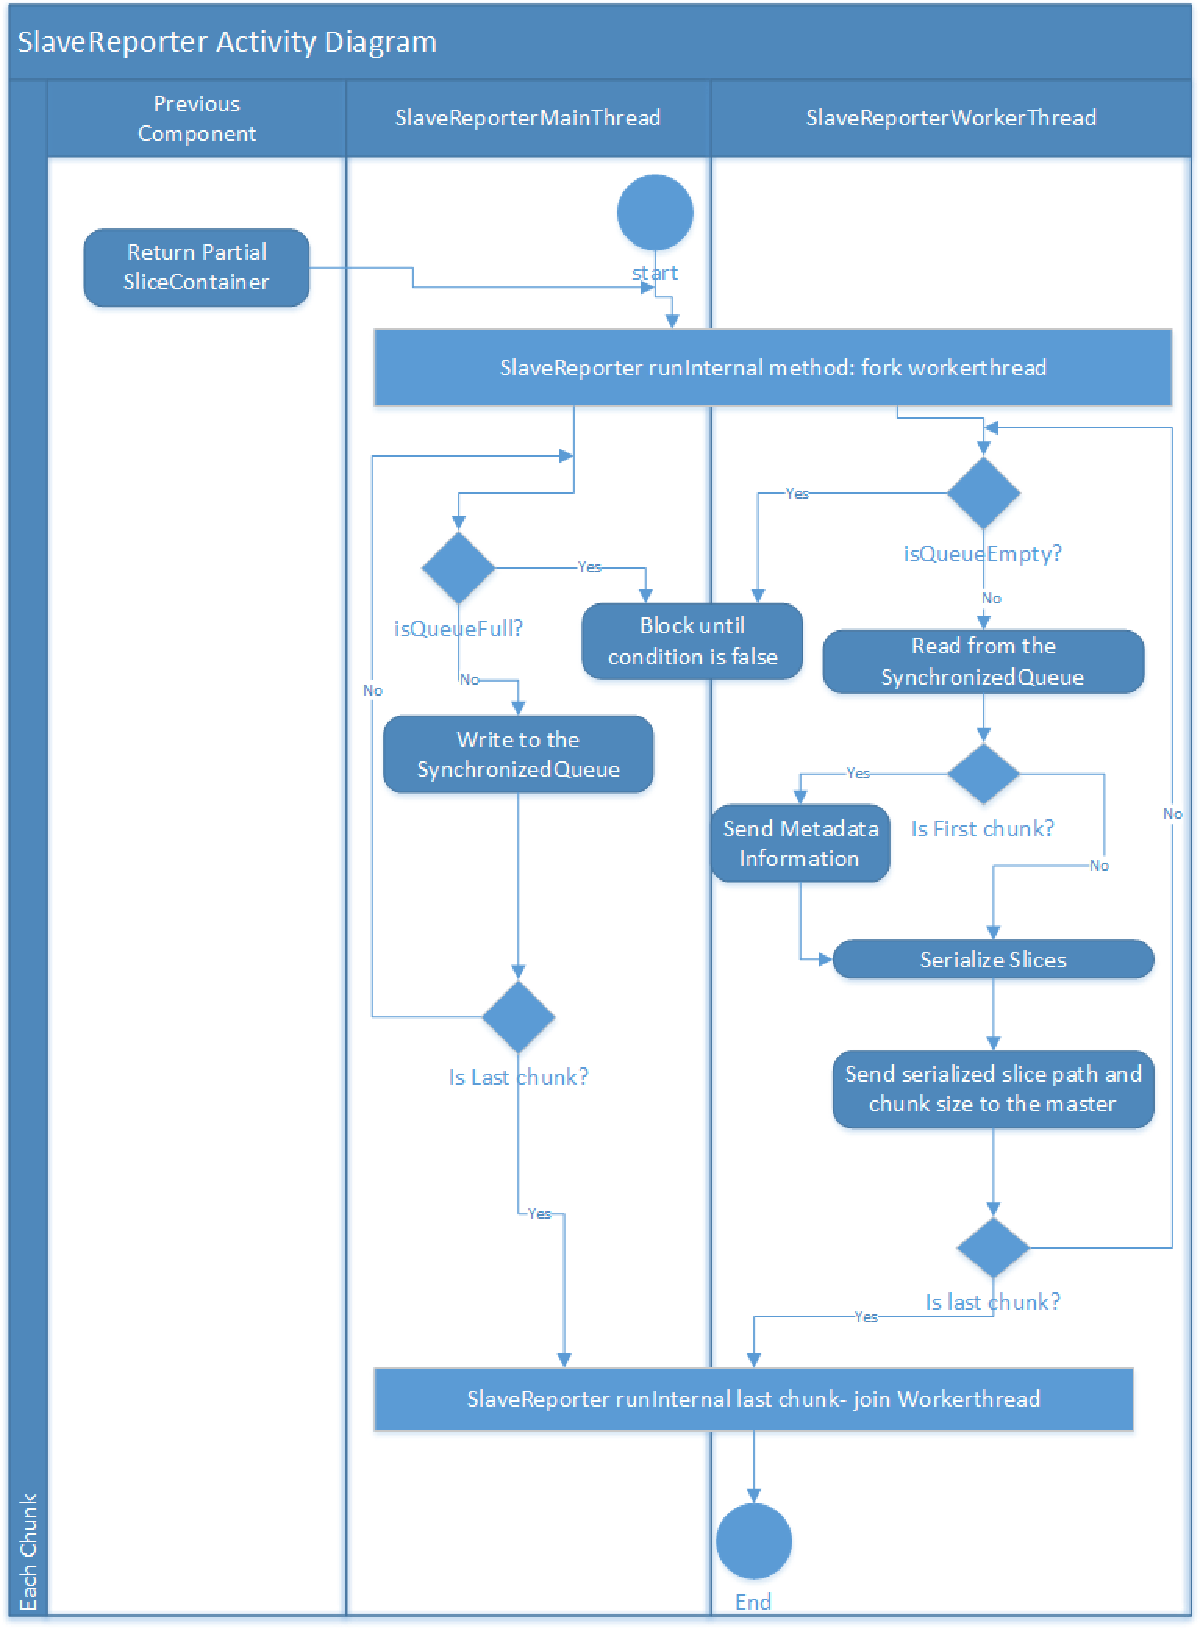
\includegraphics[scale=0.8]{SlaveReporterActivityDiagram.PNG}
\caption{\textit{SlaveReporter} Activity Diagram}
\label{fig:SlaveReporterActivityDiagram}
\end{figure}

\textbf{Analysis of component behavior}
\newline
The \textit{SlaveReporter} component is multi-threaded and uses a synchronized queue for inter-thread communication. The \textit{runInternal} method of each component is the main thread of execution i.e. the cuttlefish process, whereas in the first run of this method a worker thread is created which executes asynchronously to perform certain tasks. The main thread interacts with the next and previous components of \textit{SlavePrintingSoftware} whereas the worker thread interacts with the main thread and worker threads of \textit{MasterPrintingSoftware-MasterMerger} component. \newline

The interaction between the main thread and the worker thread can be viewed as the classic producer consumer problem, see Figure \ref{fig:ProducerConsumerProblem}, where in the main thread produces the partial slices which are consumed by the worker thread and serialized. Each chunk of partial slices is one work item produced by the main thread and inserted in the buffer. Depending on the type of buffer, there might be varying number of synchronization points between the threads. In the current design, the buffer is implemented as a queue of limited size i.e. a bounded buffer. As the buffer is of fixed size, there are two conditions which lead to blocking either the main thread or the worker thread. As the main thread acts as the producer, it blocks when the buffer is full (i.e. slow consumer) and waits on a condition indicating at least one free slot in the buffer. The worker thread acts as the consumer and blocks when there is no work item to consume and waits until there is at least one full slot. \newline

\begin{figure}[t]
\centering
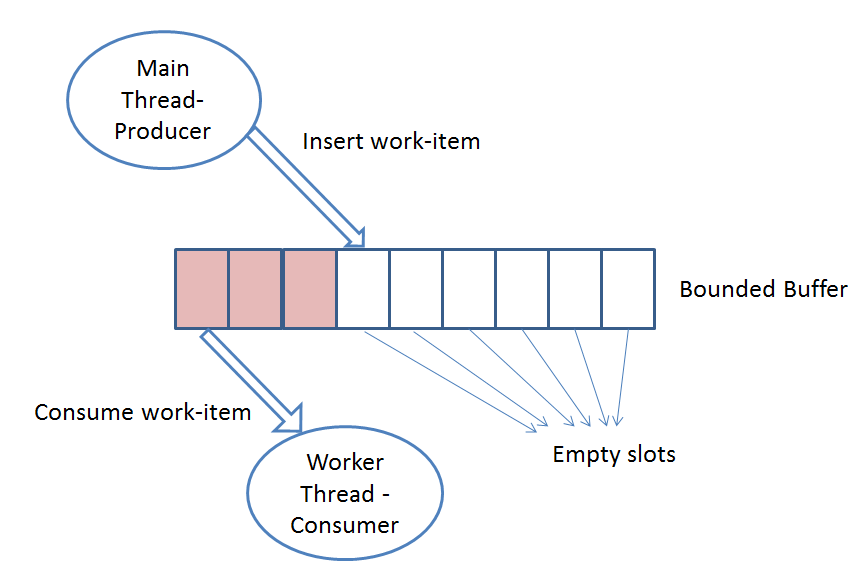
\includegraphics[scale=0.6]{ProducerConsumerProblem.PNG}
\caption{Producer-Consumer Problem}
\label{fig:ProducerConsumerProblem}
\end{figure}

The worker thread performs the task of serialization and once each chunk of slices is serialized, it communicates with worker thread of \textit{MasterPrintingSoftware-MasterMerger} component the chunk size- it acts as a way of synchronization of the worker threads between the components. The worker thread sends some meta-data  only for the first chunk of slices which includes slice height, slice width, chunk size, total number of slices. This meta-data is used by the main thread of \textit{MasterPrintingSoftware-MasterMerger} component for creating full slices.\newline

The advantages of \textit{SlaveReporter} component design are:
\begin{itemize}
\item \textbf{Separation of concerns}: The main thread is responsible for assigning the work to the worker thread and returns to continue with execution of the pipeline with the next chunk whereas the worker thread is responsible for communication and serialization.  
\item \textbf{Asynchronous communication}: The worker thread performs the blocking calls for synchronization with worker threads of \textit{MasterPrintingSoftware-MasterMerger} component. As it does so asynchronously with respect to the main thread, the communication will never lead to blocking the main thread. Both the main thread and worker thread execute in parallel.
\end{itemize} 

The disadvantages of \textit{SlaveReporter} component design are:
\begin{itemize}
\item \textbf{Synchronization Overhead}: The main thread and the worker thread need to synchronize access to the shared buffer so as to avoid race condition along with blocking calls on buffer full/ empty condition. The size of the buffer influences the performance of the solution i.e. if unlimited buffer is used the producer will never block whereas if no buffer is used there is no need for explicit synchronization as producer produces only one item and the consumer consumes it after it is produced.
\item \textbf{Increased implementation complexity}: Synchronization between the threads leads to added implementation complexity and if not managed properly might lead to deadlock. 
\end{itemize} 

\subsection{Partial Output Merging at Master} \label{MMComp}

The partial slices serialized by the slaves are de-serialized at the \textit{MasterMerger} component. The \textit{MasterMerger} component creates a worker thread per slave node in the cluster which interacts with the worker thread created by the \textit{SlaveReporter} component. The main thread of the \textit{MasterMerger} component synchronizes with worker threads at various points during the execution. The worker threads of \textit{MasterMerger} component first wait to receive the meta-data information from the \textit{SlaveReporter} component worker thread. After they have received the slice height, width, total number of slices and chunk size, they synchronize with the main thread and indicate the receipt of the meta-data. The worker threads then wait to receive the chunk size of the serialized data from the worker threads of \textit{SlaveReporter} component, the receipt of the chunk size is the indication that slices are serialized and ready for deserialization. On receiving the chunk size, they start with deserialization of the slices and create a container of deserialized partial slices. \newline

In the meantime, the main thread uses the received meta-data information from the slaves and then creates the container of the full slices. The worker threads at the master node continue to deserialize the chunk they received from the slaves and block until the container of full slices is created by the main thread and ready to be written. On signaling of availability of the container by the main thread, the worker thread then proceed with writing the partial slices to the full slices.\newline 

Each worker thread has a dedicated section in the full slice where it writes to, which helps to avoid write conflicts on the shared storage. The main thread waits until all the worker threads have finished writing the partial slices to the full slices and has container of full slices ready. The main thread then continues to proceed with the pipeline with fully merged slices whereas worker threads continue to deserialize the slices or communicate with worker threads of the slave or write the partial slices to the full slice in the container provided by the main thread. The activity diagram in the Figure \ref{fig:MasterMergerComponent} shows the activity of the main thread and worker threads of \textit{MasterMerger} component. \newline
   
The main thread at the master computes the full slice height (\begin{math}H_{\textit{f}}\end{math}), full slice width (\begin{math}W_{\textit{f}}\end{math}), offset (\begin{math}Of_{\textit{i}}\end{math}) for each worker thread (\begin{math}W_{\textit{i}}\end{math}), and total number of full slices (\begin{math}N_{\textit{f}}\end{math}). The full slice height \begin{math}H_{\textit{f}}\end{math} is computed as the addition of all the partial slice heights. If the full slice height \begin{math}H_{\textit{f}}\end{math} is exceeding the print bed height, then full slice height \begin{math}H_{\textit{f}}\end{math} is set to the print bed height- \textit{max(H)}. The height is calculated as the addition of partial slice heights because the partial slices from the slaves are written one below the other in y-axis until either the print bed height is reached or each of the slave node partial slices are placed. If the print bed height \textit{max(H)} is reached and there are still pending slave partial slices to be fit in the full slice, then the maximum partial slice width is taken as the x-offset and the remaining slices are then places along the y-axis again with each having the x-offset. The listing \ref{lst:fsh} summarizes the logic of full slice height calculation. \newline

\begin{lstlisting}[language=C++,label={lst:fsh},caption={Calculate full slice height}]
int fullsliceHt(std::vector<int> listOfpartilSliceHt)
{
	int maxAllowedHt = getPrintBedHeight(); // get the print bed height
	int totalht(0);
	for(size_t i =0;i<listOfpartilSliceHt.size(),i++)
	{
		totalht =  listOfpartilSliceHt[i] + totalHt;
	}
	if(totalht > maxAllowedHt)
	{
		totalHt= maxAllowedHt; 
		m_xOffsetNeed=true; // to indicate that x-offset will be added to some slaves
	}
	return 	totalHt;
}

\end{lstlisting}

The full slice width (\begin{math}W_{\textit{f}}\end{math}) is calculated as the maximum of the all the partial slice widths. If the total height calculated exceeds the print bed height, then total slice width is calculated as the sum of all slice widths. If the total slice width exceeds the print bed width- \textit{max(W)}, then there is no way to fit all the partial slices in the given print bed and hence some of the slaves need to be dropped. If the total slice width (\begin{math}W_{\textit{f}}\end{math}) does not exceed the print bed width \textit{max(W)}, the full slice width (\begin{math}W_{\textit{f}}\end{math}) is equal to the sum of individual partial slice widths. The full slice width calculation is summarized in the listing \ref{lst:fsw}.\newline     


\begin{lstlisting}[language=C++,label={lst:fsw},caption={Calculate full slice width}]
int fullsliceWd(std::vector<int> listOfpartilSliceWd)
{
	int maxAllowedWd = getPrintBedWidth(); // get the print bed width
	int totalWd(0);
	if(m_xOffsetNeed) // this is set to true if the total sum of slice heights > print bed height.
	{
		for(size_t i =0;i < listOfpartilSliceWd.size(),i++)
		{
			totalWd =  listOfpartilSliceWd[i] + totalWd;
		}
		if(totalWd > maxAllowedWd)
		{
			m_DropSlaves=true; // to indicate that some slaves need to be dropped
		}
	}
	else
	{
		for(size_t i =0;i < listOfpartilSliceWd.size(),i++)
		{
			totalWd = totalWd > listOfpartilSliceWd[i]? totalWd : listOfpartilSliceWd[i];
		}
	}
	return 	totalWd;
}
\end{lstlisting}

The total number of full slices is the maximum value from the received total number of slices from the slaves. The main thread needs to keep track of the individual total number of slices from each slave node so as to ensure that the master does not block for a worker thread to write to the full slices when there are no more partial slices left. 

\begin{figure}[ht!]
\centering
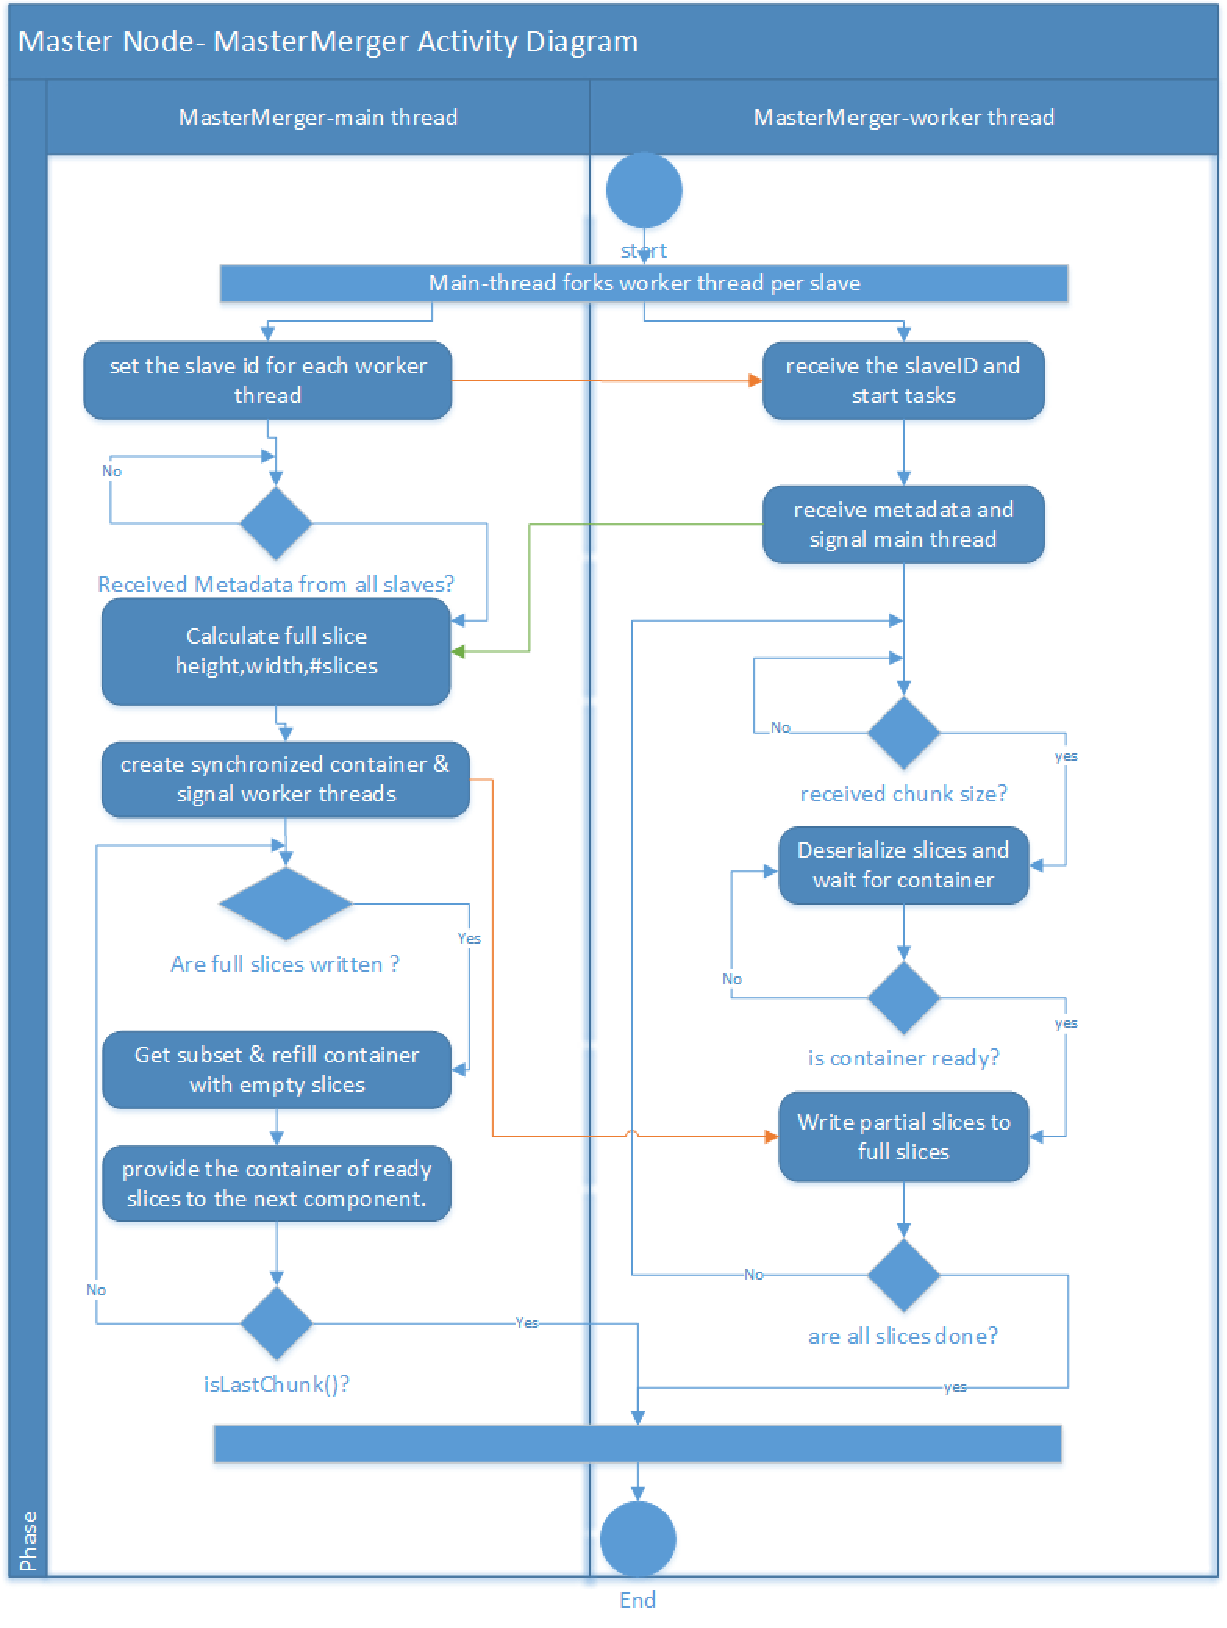
\includegraphics[scale=0.85]{MasterMergerComponent.PNG}
\caption{\textit{MasterMerger} Component- Activity Diagram}
\label{fig:MasterMergerComponent}
\end{figure}

The slice container to be provided by the main thread is a synchronized slice container which means that while removing the individual slices or subset of slices or adding the slices to the container, each thread needs to obtain the lock over the container and modify the container thereafter. The use of synchronized container ensures no data race on the shared data structure. \newline 

The advantages of the \textit{MasterMerger} component design are:  
\begin{itemize}
\item \textbf{Separation of concern}: A worker threads for each slave node helps to maintain the separation of the responsibilities among the worker threads as each worker thread is responsible for the assigned slave node.
\item \textbf{Asynchronous communication and exploiting the possible parallelism}: The worker threads for each slave node communicate with the worker thread of the \textit{SlaveReporter} component asynchronously without blocking the execution of the main thread.The worker threads perform deserialization of partial slaves and write to their assigned section in the full slices simultaneously without write conflicts amongst them. The main thread also continues to work on computing the full slice height, width etc while the worker threads are deserializing and when the worker threads are done writing to the full slice container, return the full slice container to proceed with next  component execution in the pipeline in a chunk-wise fashion. This design maintains the streaming architecture of the original non-distributed version of the pipeline. 
\end{itemize}

The disadvantages of the \textit{MasterMerger} component design are:
\begin{itemize}
\item \textbf{Synchronization Overhead}: As there are many synchronization points during the execution where either the worker threads block or the main thread block, it might lead to overhead in the execution run time. Also the synchronization leads to added code complexity. 
\item \textbf{Limited possibilities of partial slice arrangement}: As the arrangement of the partial slices in the full slices is done, there is a possibility of not achieving the optimal arrangement leading to the waste of the print area along with incapability of accommodating each slave. This might lead to dropping one or more slaves from the merging process to enable making the best possible use of the work done by the slaves.  
\item \textbf{Possibility of deadlock}: The main thread at the master blocks until each slave has received the meta-data or written to the full slices. The main thread might remain blocked if one of the slaves crashes which will eventually lead to a deadlock as other slaves might get blocked until the main thread refills the container with new empty slices. To avoid this, use of timeouts could be done. If the worker thread for a particular slave does not respond within the timeout period, then slave could be dropped. The timeouts shouldn't be too small leading unnecessary dropping of the slaves or too long leading to increased execution time overhead even when the blocking slave has crashed. The use of timeouts adds further code complexity.
\end{itemize}

\section{Prototype II- Input/Output independent of Network File System }

As discussed in the Section \ref{protoI}, the prototype I functions only if there is a shared network file system amongst the cluster nodes. The network file system is primarily used to communicate between the nodes the work load (i.e. the configuration file) and the partial output. So, to get rid of this dependency the communication between nodes must be done by sending the data through the network as a stream of bytes and not via disk I/O. The prototype II involves two major changes as compared to Prototype I: 
\begin{itemize}
\item Independence from Network File System 
\item Format of the work item allocated to the slaves
\end{itemize}  

The architecture of the distributed cuttlefish pipeline remains almost the same with two minor changes, the \textit{MasterDistributor} component is replaced by another component called as \textit{MasterPJDistributor} in the \textit{MasterPrintingSoftware}, and in the \textit{SlavePrintingSoftware}, the component \textit{SlavePJCollector} replaces the components \textit{FileParserPJ} and \textit{PrintJobOrganizer}. These changes in the printing software are explained in the following subsections. 

\subsection{Selection of the prototype}

The algorithm for performing the distributed computing progresses in the same fashion as described in the Figure \ref{lst:FC}. The configuration file submitted as input by the user to the cuttlefish application consists of a tag called as \textit{DistributionPrototype} whose value indicates the distribution prototype to be used. The valid values for this tag are 1 for prototype I and 2 for prototype II. The master node parses the configuration file and depending on the value of the \textit{DistributionPrototype} tag, it creates the components of \textit{MasterPrintingSoftware} and sends the prototype value to the slave nodes. The slave nodes wait to receive the prototype value and then add the components of \textit{SlavePrintingSoftware} depending on the received value. \newline

\subsection{Selection of Printing Software Components}
In the prototype I, the slave nodes receive the path where they could find the configuration file containing the information about of the assigned print models, texture information, component configuration for the printing pipeline and the printer specification. Just sending the prototype value is not sufficient for the slave nodes to create the \textit{SlavePrintingSoftware}. The master needs to send to each slave node all the information which was earlier contained in the main configuration file along with the information from the other files included in the main configuration file. So master should send the JSON data describing the component configuration and printer specification. Each slave node after receiving the prototype value decides what is the next information that it should wait for from the master node. For prototype I, the slave nodes wait for the main configuration file path and for prototype II, they wait for the component configuration and the printer specification description. The component configuration description depends on the user's choice of components and the configuration of each component. As the description may vary, the master first sends the size of the data followed by the data describing the component configuration. Similar to the component configuration, the printer specification description depends on the printer settings provided by the user via the printer specification file. As description of the printer specification is subject to vary depending on the available 3D printer, size of the data is sent to the slave nodes followed by the data describing the printer specification.\newline 

\subsection{Distribution of the work load to the slave nodes}

After communicating the information related to the prototype, component configuration and printer specification, the next step for the master node is to create the work load for each slave. The \textit{MasterPrintingSoftware} starts with the steps similar to prototype I i.e. parse the configuration file provided by the user and create the print job. The components responsible for doing these tasks namely, \textit{FileParserPJ} and \textit{PrintJobOrganizer}, remain unchanged. The print job is then passed to the \textit{MasterPJDistributor} component. From this point onwards the behavior of the pipeline varies for prototype II. The \textit{MasterPJDistributor} component is responsible for distributing the print jobs to the slave nodes instead of writing the configuration files per slave node. The cost function used to distribute the load amongst the nodes is the same as prototype I. The difference is the format in which the work load is assigned to the slave nodes. For each slave, a new print job containing the print objects (distributed as per the cost function) is created. Each newly created print job is a set of the print objects such that, the sum of the volumes of the print object bounding boxes is less than or equal to the threshold calculated using the cost function. The goal of the cost function is to have equal work load for each slave node so that each one of them finishes the chunk-wise computation almost at the same time.\newline

The steps performed by \textit{MasterPJDistributor} component are as follows: 
\begin{enumerate}
\item The \textit{PrintJobOrganizer} creates the print job and passes the print job to the \textit{MasterPJDistributor} component. 
\item In the \textit{MasterPJDistributor} component, the cost function is calculated using the print object bounding boxes. The calculation of the cost function is same as described in the subsection \ref{costFunc}.
\item Using the threshold calculated in the step 2, the distribution of the print objects is done such that sum of the volumes of the print object bounding boxes (assigned to each slave) is less than or equal to the threshold.
\item The set of print objects assigned to each slave is then packed into a print job per slave. 
\item The print job is then serialized to a stream of bytes and sent to the slaves. As the size of the print job may vary, the size of the serialized print job is sent to the respective slave first followed by the print job data. 
\item Each print object has texture information which is used to generate the desired appearance. The texture data is stored in the master node GPU memory when the print job is created. For the slave nodes to perform the computation and generate the partial slices correctly, the slave nodes need the texture information which should be sent by the master. The texture data size may also vary per print object and hence, the size of serialized texture data is sent first followed by the serialized texture data.   
\end{enumerate}

So to summarize the information sent by the master node to each slave node:
\begin{itemize}
\item prototype value indicating the chosen distribution type
\item size of the component configuration description 
\item component configuration description
\item size of the printer specification description 
\item printer specification description
\item size of the serialized print job 
\item serialized print job 
\item for each print object in the print job, size of texture data and texture data  
\end{itemize}

\subsection{Work Load Collection and Computation}

At the slave nodes, the first step performed is receiving the type of distribution i.e. the prototype value set by the user via the configuration file submitted to the master node. After it receives the prototype value, the slave node decides which is the next information it should wait for. For prototype II, the slave nodes wait for the component configuration. Each slave node in the cluster receives the same component configuration from the master. As the component configuration is set by the user and the size of the JSON string describing the component configuration may vary in size, the slave nodes first receive the size of the string and allocate the buffer of the appropriate size to receive the actual component configuration string. Followed by the component configuration, the slave nodes waits to receive the printer specification, similar to component configuration information, first the size of the JSON string holding the printer specification followed by the actual string. \newline   

The slave nodes then proceed to create the printing software containing the needed components. Similar to the prototype I, the \textit{SlavePrintingSoftware} does not contain any output component. As the work load received by the slaves nodes in the prototype II is a print job, The components \textit{FileParserPJ} and \textit{PrintJobOrganizer} are not included in the \textit{SlavePrintingSoftware}, instead a new component called as the \textit{SlavePJCollector} is included. The \textit{SlavePJCollector} component receives the size of the serialized print job sent by the master and allocated the buffer to receive the actual serialized print job as stream of bytes. It then deserializes the received data to create the print job. For each print object contained in the print job, it waits to receive the texture information. The slaves receive the size of the texture data, allocate the buffer for the texture data and then receive the texture data. The received texture data is then deserialized and saved in the memory of the node. The rest of pipeline remains unchanged until the \textit{SlaveReporter} component.\newline

The \textit{SlaveReporter} component, similar to the prototype I, receives the partial slices and reports them to the master node. As the nodes within the cluster do no have a shared network file system, the slices which are reported to the master node are in form of stream of bytes instead of files written to the disk. The value of the selected distribution type is set at the time \textit{SlavePrintingSoftware} creation as \textit{persistent} data- it is a piece of information accessible by all the components of the pipeline. \textit{SlaveReporter} fetches the prototype value from the persistent storage before it proceeds with rest of the computation. \newline

The \textit{SlaveReporter} component sends the meta-data information which is the partial slice height, width, total number of slices for the assigned work load and first chunk size. For the prototype II, it skips sending the path where the master node would find the partial slice file. For each chunk of partial slices to be sent to the master, the slave begins by informing the size of the chunk followed by serialization of the slices. Through serialization of the slices it converts the slices to stream of bytes. The size of the serialized slice is sent to the master which allows the master to allocate the buffer of appropriate size and then send the serialized slice data. The \textit{SlaveReporter} component design remains unchanged and is as described in the subsection \ref{SRepoComp}.

\subsection{Creation of the full slices}

At the master node, after assigning the work load to the slave nodes, the \textit{MasterMerger} component is executed. It is in charge of collecting the partial slices from the slave nodes and merging them to form full slices. The \textit{MasterMerger} component, similar to the \textit{SlaveReporter} component, fetches the prototype value from the persistent storage which is saved when the instance of the \textit{MasterPrintingSoftware} is created. There is no huge difference in how the component performs the merging of the partial slices but rather how it receives the partial slices from the slave nodes. The component design remains unchanged and is as described in the subsection \ref{MMComp}. Each worker thread begins by receiving the meta-data information from their respective slave node. For the prototype II, the worker thread does not receive the path where the partial slices files are written by the slave. After receiving the chunk size, the worker threads receive the size of the stream of bytes slice-wise, allocate the buffer and receive the stream of bytes. They then deserialize the stream of bytes to partial slice and store them in the partial slice container. The rest of the steps until the merging of partial slices to full slice and passing them to the output component remains unchanged.

The information communicated between the master and slave nodes is summarized in the Figure \ref{fig:ProtoII}.

\begin{figure}[!t]
\centering
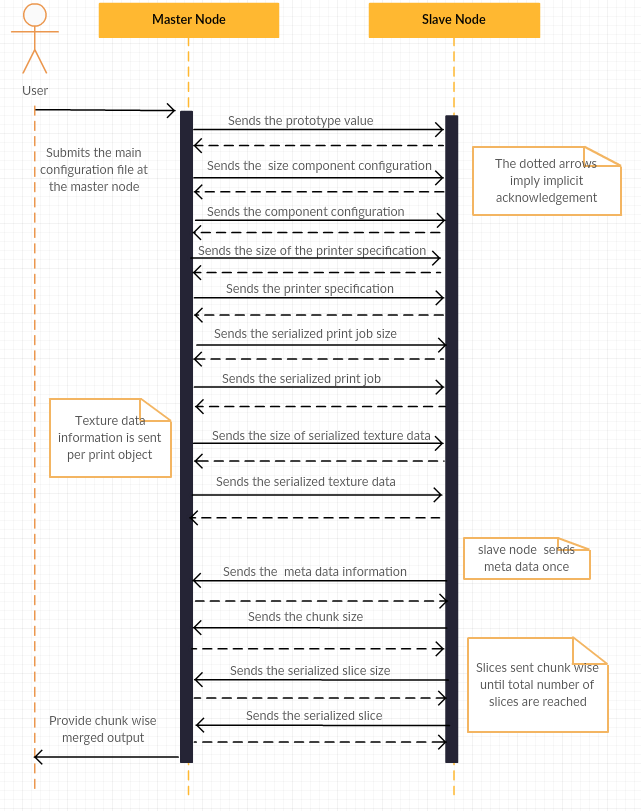
\includegraphics[scale=0.85]{ProtoII_SequenceDiagram.PNG}
\caption{Communication between slave and master nodes}
\label{fig:ProtoII}
\end{figure}


\section{Serialization and Deserialization of Data}

The nodes forming the cluster used for distributed computing may not always be homogenous, which means that each node may be different in terms of the system architecture, computation capacity and memory. Due to such heterogeneity, the representation of the user defined data types (i.e. in our case objects) may vary as the "endianness" of the nodes might differ \cite{ObSerDeser}. To ensure that each node interprets the data correctly, the objects are "flattened" to stream of bytes or a string before sending it the destination, also known as serialization of the objects. At the destination node, the received stream of bytes are "unflattened" to reconstruct the objects, which is known as deserialization \cite{yadav2016system}. The Figure \ref{fig:SerDeser} summarizes the serialization and deserialization process used in cluster computing.

\begin{figure}[!t]
\centering
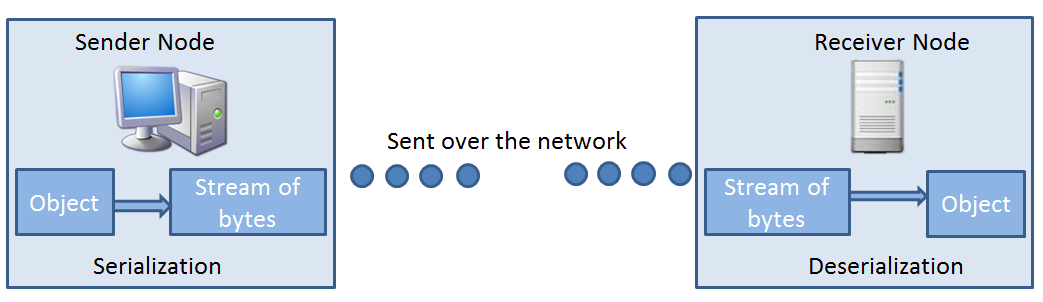
\includegraphics[scale=0.65]{SerDeser.PNG}
\caption{Serialization and Deserialization}
\label{fig:SerDeser}
\end{figure}
  
\newpage
	
\chapter{Implementation}

The design for the prototype I and prototype II detailed in the chapter \ref{DA} were implemented through iterative development process where the design for prototype I was drafted and implemented first, followed by the prototype II. This chapter details the procedure which was followed during the development and implementation of the thesis.  

\section{Native Cuttlefish Application} 
The native cuttlefish application is a 64-bit windows application, developed in C++ language using the Microsoft Visual Studio 12 SDK and the compiler used to build the code is Microsoft C/C++ V120 compiler. A project could be compiled either as static library or an executable in release or debug mode. The input for the application i.e. the path of the main configuration file, is presented as command line argument. The output generated by the application depends on the type of output component chosen in the component configuration. For each component, the behavior of the component is logged in the performance report and a log file for overall pipeline is written to the working directory at the end of the execution. This helps to analyze the component performance as well as to know the possible error by looking into the pipeline execution trace in case of a failure. Some of the projects of the application use external libraries (like zlib, little cms , poly2tri, boost, itk etc) which are either used as headers only or compiled for windows platform and linked as static library. 

Some parts of the computation performed by the application is on the GPU (graphics processing unit) and the code performing this computation is written and compiled using CUDA Toolkit. Another library used by the application is OpenGL(Open Graphics Library) wherein various powerful visualization features of the library are used for rendering, texture mapping etc. The minimum OpenGL version that is needed by the application to run should be 2.0 as one of the APIs used- glCreateProgram, is available only in version 2.0 or higher. The native application has a strong dependency on availability of graphics library and CUDA.     

\section{Prerequisites for Distributed Cuttlefish Application Development} 

The goal of the thesis was earlier to provide a cloud service which could take the input from the user and do the computation using the cloud instances and provide the bitmaps as the output. With this goal, the native application had to be modified such that it could run on the cloud instances provided by the AWS (Amazon Web Services) as PAAS (Platform as a Service). The cluster of instances which formed the {\lq}cloud{\rq} were the basic Amazon EC2 instances which were virtual machines with Linux operating system. As the basic instances were virtual machines which were not GPU accelerated i.e. they did not have access to a GPU, and therefore the code which performed the GPU computing had to be changed such that only when the GPU is available, the code is compiled and used . So, this change to the native application code was done by creating a new configuration, other than release and debug, called as the CUDA\_FREE\_CONFIG which got rid of the dependency on availability of CUDA on the system running the application. The code performing the GPU computing is defined under if-defs to get the CUDA\_FREE\_CONFIG as seen in the Listing \ref{lst:CFC}

\begin{lstlisting}[language=C++,label={lst:CFC},caption={CUDA free configuration}]
//....
#ifndef CUDA_FREE	
			inline operator std::shared_ptr<VoxelSliceGPU>()
			{
				if (m_channel == m_invalidIndex)
					return nullptr;
				validate();
				return std::dynamic_pointer_cast<VoxelSliceGPU>(m_pContainer->m_slices[m_channel][m_slice]);
			}

#endif
//....
\end{lstlisting}

The CUDA\_FREE\_CONFIG configuration was still only for windows platform and the projects needed to be compiled such that they were compatible with Linux and it was necessary to get rid of the windows specific dependencies. To achieve portability and make the cross-platform build of the application possible, a configuration file called as the {\lq}CMakeLists.txt{\rq}  was written for each project of the application. Using CMake, an open-source system that manages the build process for an operating system in a compiler independent manner, all the project's cmakelists.txt files were parsed to generate the desired solution (depending on the generator chosen by the developer) i.e. the solution file could be Microsoft Visual Studio 12 solution or Unix makefiles or Eclipse CDT Unix makefiles. After using cmake to generate makefiles for linux system, the process to remove the windows specific code was started but could not be completed  due to time limitation (as it required rigorous amount changes). Hence, instead of using basic EC2 instances running Linux, a decision to use basic EC2 instances running windows operating system was made.    

The next step was to check if the CUDA free application configuration could run on an instance i.e. virtual machine with windows operating system. The application crashed in the call to the glCreateProgram api on the instance as the OpenGL version was 1.1. The fix for this issue would be to make OpenGL version 2.0 available on the instance i.e. the Virtual Machine. This cannot be done as OpenGL has a hardware limitation and the virtual machines use virtual GPUs which cannot support OpenGL 2.0 and provide support for only GPU basics. Hence, as most of the basic cloud instances (irrespective of the vendor/provider) are virtual machines supporting only GPU basics, the application could not be run on these instances. Therefore, instead of using a cloud of virtual machines as compute nodes, a decision to use physical processors as compute nodes was made, hence instead of cloud computing, cluster computing was chosen as the distributed system . 

The physical processors are 64-bit machines which run windows operating system and have access to the GPUs with the OpenGL 2.0 version available to the application. These physical machines are connected via the enterprise network. Though the compute nodes already had a common network, to use them as a cluster there was a need to perform a few installations to enable `clustering` as detailed in the section \ref{ICS}. 


\section{Installation and Cluster Set-up} \label{ICS}

To begin with, a cluster with 2 nodes was created such that the nodes were connected to each other via a common network. To check if the cluster nodes could communicate, a simple ping test was performed. The next step was to write a program which performed a simple task in a distributed fashion and to run it on the cluster. For the cluster to work as system where the processing can be shared, there needs to be a way in which the cluster nodes can be named and the work to be done by each node could be distinguished i.e. assign roles to the nodes. There are many types of hardware/software solutions for the cluster which enable naming and role distinction among cluster nodes. The decision to use MPI-Message Passing Interface, was made to achieve naming and role assignment amongst the cluster nodes. MPI is the open standard specification for message passing libraries which provide apis to enable communication, role distinction and naming amongst the cluster nodes. There are various implementations of the specification available which basically perform the same thing i.e. message passing amongst the cluster nodes but are different with respect to the platform they support, commands to compile and launch the program, debugging and developed by different institutions. 
Some of the implementations are free-ware and some aren\textquotesingle t. As currently, cuttlefish is a windows application developed using Microsoft visual studio, the Microsoft\textquotesingle s implementation of MPI called as MSMPI is used. 

To use MSMPI, on each node of the cluster, the MS-MPI SDK is downloaded and installed. To verify if the installation and setup is done correctly, the environment variables are checked using the command {\lq} set MSMPI {\rq}. The environment variables which are particularly interesting are \$MSMPI\_INC\$, \$MSMPI\_BIN\$, and \$MSMPI\_LIB64\$. The table \ref{MSMPI-ENV} summarizes the details about these variable. 

\begin{table}[]
\centering
\label{my-label}
\begin{tabular}{|l|l|l|ll}
\cline{1-3}
\begin{tabular}[c]{@{}l@{}}Environment\\ Variable\end{tabular} & Value                                       & Significance                                 &  &  \\ \cline{1-3}
MSMPI\_INC                                                     & ..\textbackslash Microsoft SDKs\textbackslash MPI\textbackslash Include               & Path to find the headers                     &  &  \\ \cline{1-3}
MSMPI\_LIB64                                                   & ..\textbackslash Microsoft SDKs\textbackslash MPI\textbackslash Lib\textbackslash x64\textbackslash & Path to find the libraries for 64 bit system &  &  \\ \cline{1-3}
MSMPI\_BIN                                                     & ..\textbackslash Microsoft MPI\textbackslash Bin\textbackslash          & Path to find the binaries                    &  &  \\ \cline{1-3}
\end{tabular}
\label{MSMPI-ENV}
\caption{ MS-MPI Environment Variable}
\end{table}

To compile a program which is designed to run on the cluster where the nodes communicate using MPI, the directories which help to resolve the reference to header files specific to MPI and path to the libraries which resolve linking to the MPI functions are incorporated in the project. Before running the program, a process management system which allows to manage the parallel processes on the cluster nodes should be executed on each of the cluster node. For MPI, the process management system used is called as SMPD (Simple Multipurpose Daemon) which is part of the software component of the process manager provided by Intel. It allows starting and managing parallel jobs on the cluster nodes. SMPD is used as a windows service and is set during the MPI installation. Ideally, the version of SMPD running on each node in the cluster should be same, although if there are different versions of SMPD, there is a possibility to disable the check for the versions. As the SMPD service is set during MPI installation, the version of SMPD is compatible with the mpiexec version. To run the program, mpiexec command is used with the arguments specifying the number of hosts, host names, the directory where the executable for application to be launched is available, the name of the executable followed by arguments to the executable. The listing \ref{lst:MPIC} is an example of the command syntax to launch the application using mpiexec command.  

\begin{lstlisting}[language=C++,label={lst:MPIC},caption={mpiexec syntax}]
mpiexec -hosts 2 PC2215 PC2286 -wdir \\pc2215\bin\Release\ Cuttlefish.exe \\pc2215\mainconf.json
\end{lstlisting}  
	
\section{Introduction to New Components}

After the set-up and installation, the next step was the implementation of the prototype I followed by the implementation of prototype II. The components of both the prototypes are discussed in detail in the chapter \ref{DA}. Each of the new component is inherited from the class called as the \textit{PrintingComponent} and is registered using the component name. During the creation of the pipeline i.e. when the component configuration is parsed, each of the component is created and initialized with the required parameter values. The parameter values for each component are set in the configuration file. The Figure \ref{fig:Componentdiagram} summarizes the new components(underlined component names) introduced during the implementation of the thesis.

\begin{figure}[ht!]
\centering
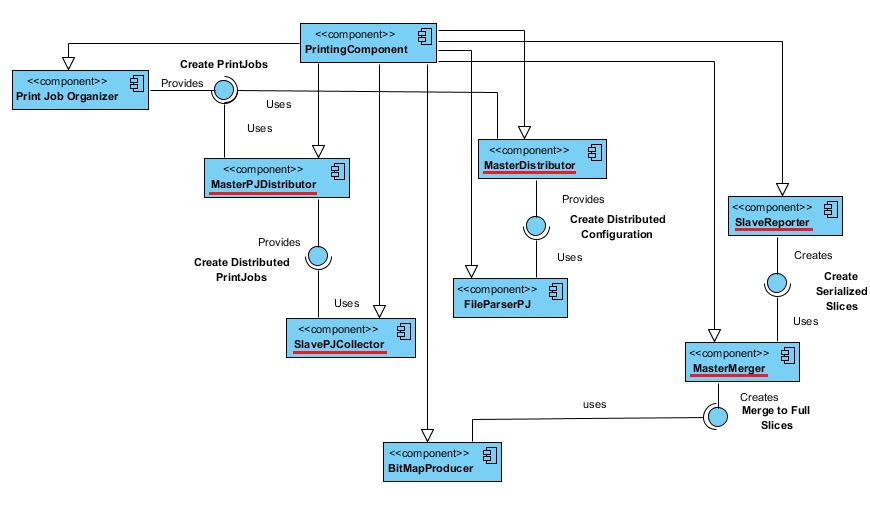
\includegraphics[scale=0.8]{Componentdiagram.PNG}
\caption{Component Diagram For New Components}
\label{fig:Componentdiagram}
\end{figure}

Each component has an input it receives from another component and an output that it generates which may be used by the following component in the pipeline(if any). The dependency is depicted in the Figure \ref{fig:Componentdiagram} by the {\lq}lollipop{\rq} symbol where in the half circle depicts interface exported by the component and the circle represents the interface that is imported by the component, for example, the component \textit{MasterDistributorPJ} uses the print job created by the \textit{PrintJobOrganizer} and provides the print jobs with distributed print objects used by the \textit{SlavePJCollector}.

\subsection{Introduction to the New Classes}
The new classes which were implemented during the thesis are enlisted in the Table \ref{CSPI} for prototype I, in the Table \ref{CSPII} for prototype II and common classes used by both the prototypes are listed in Table \ref{ComClass}. 

\begin{table}[ht]
\centering
\caption{Class specific for Prototype I}
\label{CSPI}
\begin{tabular}{|l|l|l}
\cline{1-2}
\textbf{Class}              & 
\textbf{Purpose}                                                                                                                                                                                                &  \\ \cline{1-2}
MasterDistributor & \begin{tabular}[c]{@{}l@{}}Class for slave work item creation and distribution. \\ The work item created is the main configuration file \\ containing the assigned number of print object files.\end{tabular} &  \\ \cline{1-2}
\end{tabular}
\end{table}

\begin{table}[ht]
\centering
\caption{Classes specific for Prototype II}
\label{CSPII}
\begin{tabular}{|l|l|l}
\cline{1-2}
\textbf{Class}      & \textbf{Purpose}                                                                                                                                                                   &  \\ \cline{1-2}
MasterPJDistributor & \begin{tabular}[c]{@{}l@{}}Class for creation of print jobs with the print objects \\ distributed using the cost function and \\ serialization of the print jobs\end{tabular}      &  \\ \cline{1-2}
SlavePJCollector    & \begin{tabular}[c]{@{}l@{}}Class for collection of the serialized print job, \\ de-serialization of the print jobs and loading\\ the texture data to the node memory.\end{tabular} &  \\ \cline{1-2}
\end{tabular}
\end{table}

\begin{table}[ht]
\centering
\caption{Common Classes For Prototype I and II}
\label{ComClass}
\begin{tabular}{|l|l|l}
\cline{1-2}
\textbf{Class}                & \textbf{Purpose}                                                                                                                                                           &  \\ \cline{1-2}
MasterPrintingSoftware        & Creates and manages the printing software for the master node                                                                                                              &  \\ \cline{1-2}
SlavePrintingSoftware         & Creates and manages the printing software for the slave node                                                                                                               &  \\ \cline{1-2}
P3DNetworkComm                & Interface exposing the methods for communication                                                                                                                           &  \\ \cline{1-2}
P3dNetworkCommMPI             & \begin{tabular}[c]{@{}l@{}}Implements the interface methods using MPI as \\ the message passing library\end{tabular}                                                       &  \\ \cline{1-2}
DistributedComponentParser    & Parser for the JSON files used for distributed computing                                                                                                                   &  \\ \cline{1-2}
DistributedComponentInitiator & \begin{tabular}[c]{@{}l@{}}Initiator class for distributed computing. It manages \\ the cluster creation, execution and shut down of the\\ printing software\end{tabular}  &  \\ \cline{1-2}
SyncVoxelSlicesContainer      & \begin{tabular}[c]{@{}l@{}}Synchronized voxel slice container allowing \\ synchronous access to multiple threads\end{tabular}                                              &  \\ \cline{1-2}
MasterMergerWorker            & \begin{tabular}[c]{@{}l@{}}Interface exposing methods for performing \\ collection of metadata, de-serialization and\\  writing partial slices to full slices\end{tabular} &  \\ \cline{1-2}
MasterMergerWorkerImpl        & \begin{tabular}[c]{@{}l@{}}Implementation of the MasterMergerWorker class \\ with a thread per slave\end{tabular}                                                          &  \\ \cline{1-2}
DistributedCostFunction       & \begin{tabular}[c]{@{}l@{}}Class for calculation of the threshold and cost \\ function used for load distribution\end{tabular}                                             &  \\ \cline{1-2}
SlaveReporter                 & \begin{tabular}[c]{@{}l@{}}Class which performs serialization of the slices \\ and reports them to master\end{tabular}                                                     &  \\ \cline{1-2}
MasterMerger                  & \begin{tabular}[c]{@{}l@{}}Class performing collection of partial slices \\ and generation of merged full slices\end{tabular}                                              &  \\ \cline{1-2}
SlaveDataBuffer               & Synchronous queue used by the thread of slave reporter class                                                                                                               &  \\ \cline{1-2}
\end{tabular}
\end{table}

\begin{table}[ht]
\centering
\caption{Projects for Distributed Computing}
\label{ProDC}
\begin{tabular}{|l|l|l|ll}
\cline{1-3}
Project                  & Components / Classes                                                                                                              & Properties                                                                                                                                                                                                                                                                                                                   &  &  \\ \cline{1-3}
P3DDistributedCuttlefish & \begin{tabular}[c]{@{}l@{}}MasterMerger\\ MasterDistributor\\ MasterPJDistributor\\ SlaveReporter\\ SlavePJCollector\end{tabular} & \begin{tabular}[c]{@{}l@{}}1.Project contains the components which are \\ implemented for distributed computing. \\ 2.The project is built as a dynamic linking library. \\ 3.The project uses the Zlib, rapidjson external libraries.\end{tabular}                                                                      &  &  \\ \cline{1-3}
P3DDistributedUtility    & \begin{tabular}[c]{@{}l@{}}MasterPrintingSoftware\\ SlavePrintingSoftware\\ DistributedComputingInitiator\end{tabular}            & \begin{tabular}[c]{@{}l@{}}1. Project contains the classes implementing the \\ printing software and the initiator class for\\ distributed computing\\ 2.The project is built as a static library. \\ 3.The project uses rapidjson external library.\end{tabular}                                                     &  &  \\ \cline{1-3}
P3DNetworkComm           & \begin{tabular}[c]{@{}l@{}}P3DNetComm\\ P3DNetCommMPI\end{tabular}                                                                & \begin{tabular}[c]{@{}l@{}}1.Project contains the interface exporting the \\ methods used for communication over the network \\ and an MPI specific implementation of the interface. \\ 2.The project is built as a dynamic linking library\\ 3.MS-MPI library is the external library used \\ in the project.\end{tabular} &  &  \\ \cline{1-3}
\end{tabular}
\end{table}


\subsection{Code Organization}

The solution for the application is generated using the CMAKE tool with each project having it's own CMakeLists.txt file. The CMakeLists.txt file specifies the properties of the project such as the project would be built as an executable or static library or dynamic library, the libraries it needs to linked to, the include directories etc. Through the thesis, the code written is organized in 3 different projects namely P3DDistributedCuttlefish, P3DDistributedUtility and P3DNetworkComm. The Table \ref{ProDC} describes code organization in the projects named. Some of the directives of CMake which influence the generator output of a project are add\_library, add\_subdirectory, target\_link\_library  and add\_dependencies. The Table \ref{CDirec} details the directive used.

\begin{table}[]
\centering
\caption{Cmake Directives}
\label{CDirec}
\begin{tabular}{lll}
\hline
\multicolumn{1}{|l|}{\textbf{Cmake Directive}} & \multicolumn{1}{l|}{\textbf{Purpose}}                                                                                                                                                                                                          & \multicolumn{1}{l|}{\textbf{Example}}                                                                                                                                                                                                                                                                                                                                                                                                                                                                                                                                                                                                                                                                                                                                                                              \\ \hline
\multicolumn{1}{|l|}{add\_library}             & \multicolumn{1}{l|}{\begin{tabular}[c]{@{}l@{}}1.Adds a library with the stated \\ target name to be built from\\ the listed source code.\\ 2. The library could be static library, \\ dynamic linking library or modules.\end{tabular}}       & \multicolumn{1}{l|}{\begin{tabular}[c]{@{}l@{}}add\_library(P3DDistributedCuttlefish SHARED\\                     SRC\_FILES  SRC\_HDRS\\                     DEPEND\_INCLUDES)\\ \\ The project P3DDistributedCuttlefish is \\ added as dynamic linking library (SHARED keyword\\ specifies creation of dynamic linking library to the cmake\\ tool), followed by the source files, header files and other \\ includes needed to build the project. \\ \\ add\_library(P3DDistributedUtility STATIC \\                     SRC\_FILES  SRC\_HDRS\\                     DEPEND\_INCLUDES)\\ \\ \\ The project P3DDistributedUtility is added as a static \\ library specified by the use of STATIC keyword followed\\ by the source files, header files and included needed to \\ build the project.\\ \end{tabular}} \\ \hline
\multicolumn{1}{|l|}{add\_dependencies}        & \multicolumn{1}{l|}{\begin{tabular}[c]{@{}l@{}}1. Adds the dependency among \\ the projects.\\ 2. It helps to ensure that the projects\\ on which the current project is \\ dependent on is build before the \\ current project.\end{tabular}} & \multicolumn{1}{l|}{\begin{tabular}[c]{@{}l@{}}\$\{DEPEND\_INCS ../P3DInfrastructure;../P3DUtility;\\                                 ../P3DModuleInterface;\\                                 ../P3DNetComm;\}\\ \\ \\ add\_dependency(P3DDistributedCuttlefish \\                             DEPEND\_INCS)\\ \\ The project P3DDistributedCuttlefish is dependent \\ on the projects P3DInfrastructre, P3DUtility,\\ P3DModuleInterface and P3DNetComm. \\ add\_dependency ensures that these projects are\\ built before P3DDistributedCuttlefish is built.\\ \end{tabular}}                                                                                                                                                                                                                                      \\ \hline
\multicolumn{1}{|l|}{add\_subdirectory}        & \multicolumn{1}{l|}{\begin{tabular}[c]{@{}l@{}}1.Adds the specified subdirectory \\ in the solution.\\ 2.The name of the directory specifies \\ the location of the source \\ CMakeLists.txt and source \\ code files.\end{tabular}}           & \multicolumn{1}{l|}{\begin{tabular}[c]{@{}l@{}}add\_subdirectory(P3DDistributedCuttlefish)\\ \\ The directive specifies that the project \\ P3DDistributedCuttlefish should be added to \\ the current solution generated and the\\ CMakeLists.txt file required to include\\ the project is present in the directory with\\  same name as the project. \\ \end{tabular}}                                                                                                                                                                                                                                                                                                                                                                                                                                              \\ \hline
\multicolumn{1}{|l|}{target\_link\_libraries}  & \multicolumn{1}{l|}{\begin{tabular}[c]{@{}l@{}}1.Links the specified libraries\\ to the named target.\end{tabular}}                                                                                                                            & \multicolumn{1}{l|}{\begin{tabular}[c]{@{}l@{}}\$\{DEPEND\_LIBS ../zlib.lib;../msmpi64.lib\}\\ \\ target\_link\_libraries\{P3DNetComm DEPEND\_LIBS\}\\ \\ The project P3DNetComm is included in the \\ solution is built as a dynamic link library and \\ the target dynamic linking library generated\\ will be linked to the zlib library and msmpi\\  lib 64 bit version. \\ \end{tabular}}                                                                                                                                                                                                                                                                                                                                                                                                                         \\ \hline
                                               &                                                                                                                                                                                                                                                &                                                                                                                                                                                                                                                                                                                                                                                                                                                                                                                                                                                                                                                                                                                                                                                                                   
\end{tabular}
\end{table}

While using CMake tool to generate the solution for distributed cuttlefish application, the flag P3D\_DISTRIBUTED should be enabled which allows the inclusion of the projects which have the distributed computing implementation. The flag is defined so as to help easy solution generation of both distributed and native cuttlefish application. When the flag is set, the sub-directories are added by using the add\_subdirectory directive in the CMakelists.txt. The Listing \ref{lst:DIST} shows how the sub-directories are included and the use of the flag.

\begin{lstlisting}[language=C,label={lst:DIST},caption={Flag to enable distributed computing solution}]
if(DEFINED P3D_DISTRIBUTED)
	add_subdirectory(P3DDistributedCuttlefish)
	add_subdirectory(P3DDistributedUtility)
	add_subdirectory(P3DNetComm)
endif()
\end{lstlisting}

The MPI dependencies are managed by using the find\_package directive in the CMakeLists.txt of the target project. The Listing \ref{lst:MPIFind} is shows how to find about availability of MPI and if MPI is available, include the headers as well as link to the library. 

\begin{lstlisting}[language=C,label={lst:MPIFind},caption={find\_package use for MPI libraries}]
find_package(MPI REQUIRED)
if(MPI_FOUND)
	include_directories(${MPI_INCLUDE_PATH})
	target_link_libraries( P3DDistributedCuttlefish ${MPI_LIBRARIES})
endif(MPI_FOUND)
\end{lstlisting}

\section{Communication Specifics}

\textbf{M}icrosoft \textbf{M}essage \textbf{P}assing \textbf{I}nterface (MS-MPI) is Microsoft's windows specific implementation of Message Passing Interface Specification  (MPI-2 version). It provides 160 APIs which allow communication in a distributed computing environment by use of message passing paradigm and help to build application which perform parallel computation. This section details the API's used in the implementation followed by a brief explanation of how MS-MPI works internally and last but not the least comparison with other communication mechanisms.

\subsection{MPI APIs used in the Implementation} \label{MSMPI-API} 

A parallel program written using MPI first should initialize the MPI execution environment which allows to perform the following:
\begin{itemize}
\item Create, initialize and set up a message passing layer
\item Launch the stated number of processes
\item Allocation of resources such as shared memory (if required), local inter-process communication channels,
network communication channels and to allow communication with specialized network hardware it allocates {\lq}special{\rq} memory.  
\end{itemize}

If the initialization of the MPI execution environment fails due to failure in one of the above steps, the command hangs or aborts depending on the chosen implementation. For MS-MPI, there some warning messages shown on the command prompt. The initialization is done using MPI\_INIT method as seen in the Listing \ref{lst:mpiINIT}. 

\begin{lstlisting}[language=C++,label={lst:mpiINIT},caption={Initialization of Execution Environment}]
#include<mpi.h>
void MPI::Init(int& argc, char**& argv)
void MPI::Init()
\end{lstlisting}

The thread that calls the MPI\_INIT should also be the thread which destroys the set-up by calling MPI\_FINALIZE. MPI\_INIT should ideally be the first method to be called before any kind of communication can be done within the distributed computing environment, although MPI\_INITIALIZED - checks if MPI environment is initialized by calling MPI\_INIT, MPI\_FINALIZED - checks if the set-up has be been destroyed by calling MPI\_FINALIZE, MPI\_GET\_VERSION - gets the MPI standard followed by the current implementation, can be called before MPI\_INIT. \newline

The set of processes launched during the initialization process form a communicator and each process has rank within the communicator.
The query functions like MPI\_COMM\_SIZE and MPI\_COMM\_RANK are local functions which do not require coordination and communication outside the local MPI process as they are local look ups. MPI\_COMM\_SIZE returns the size of communicator created during the  MPI\_INIT method execution and MPI\_COMM\_RANK returns the rank of process, executing the instruction, in the communicator. The implementation decides the order in which the ranks are assigned to the processes and generally the node on which mpiexec is executed has the rank 0 which is the rank of the root/master process. The Listing \ref{lst:mpicommSizeRank} shows the syntax of the MPI\_COMM\_SIZE and MPI\_COMM\_RANK methods.

\begin{lstlisting}[language=C++,label={lst:mpicommSizeRank},caption={MPI Query Functions}]
#include <mpi.h>
int Comm::Get_size() const
int Comm::Get_rank() const
\end{lstlisting}

Message passing is done through fundamental directives called as send and receive. As the name suggest, the send directive is used to send information and receive directive is used to receive the information. The communication when done using the send and receive directives is point to point communication as there is one sender and one receiver for each pair of send and receive. The communication can also be a broadcast where in there is one sender and rest of the processes in the communicator are receivers. In the implementation of the thesis, point to point communication is done using MPI\_SEND and MPI\_RECEIVE methods. \newline

The directives for point-to-point communication come in two different flavors, blocking and non-blocking. The blocking send and receive can have 3 additional modes of communication namely, buffered, synchronous and ready. The blocking send does not return from the call until the message data and envelope has been safely stored and the message buffer is ready to be modified again \cite{mpiMech}. The blocking send does not provide a status of message being sent or received but rather just provides a guarantee that the message buffer is available again.  The Listing \ref{lst:mpiSend} provides the syntax of a blocking send call. The first three arguments- pointer to the buffer holding the message data, count of elements stored in the buffer and the type of each element in the buffer form the message content where as the last three arguments namely the destination i.e. the rank of the receiving process, the tag- a unique number identifying the message and communicator handle form the message envelope. \newline  

\begin{lstlisting}[language=C++,label={lst:mpiSend},caption={Blocking MPI Send}]

int MPI_Send(void* buf, int count, MPI_Datatype datatype, int dest,int tag, MPI_Comm comm)

void MPI::Comm::Send(const void* buf, int count, const MPI::Datatype& datatype, int dest, int tag) const  	
\end{lstlisting}

The blocking receive consists of 6 parameters, the first three include the pointer to receiver's buffer, the size of the data to be received also the size of the buffer and the type of data to be received and the following 3 parameters include rank of the sender process i.e. the source of the sender, tag is the unique number identifying the message and communicator to which the process belongs to.  The receiver can receive message from {\lq}any{\rq} source where as the sender always has to specify the receiver of the message which is known as the {\lq}push{\rq} mode. If the receiver had to always mention a specific sender then such a communication mode is called the {\lq}pull{\rq} mode. MPI\_STATUS can used to know the status of the receive call and if in a buffer under run error case the MPI\_STATUS value is MPI\_ERROR which can be used for further investigation. 

\begin{lstlisting}[language=C++,label={lst:mpiReceive},caption={Blocking MPI Receive}]
int MPI_Recv(void* buf, int count, MPI_Datatype datatype, int source, int tag, MPI_Comm comm, MPI_Status *status)

void MPI::Comm::Recv(void* buf, int count, const MPI::Datatype& datatype, int source, int tag, MPI::Status& status)
\end{lstlisting}

The blocking send and receive work in tandem. For every send there needs to be corresponding receive matching in the following triples  source (rank), tag and communicator. MPI specification 2.0 provides the following properties for the point-to-point communication paradigm. 

\begin{itemize}
\item \textbf{Order}- The message ordering is needed to maintain the requirement of matching send and receives. The messages are non-overtaking which makes the code for message exchanges deterministic in a single-threaded implementation. 
\item \textbf{Progress}- This guarantees completion of send and receive operations if there is matching pair of send and receive operation.  
\item \textbf{Fairness}- No guarantee of fairness in managing the communication is provided.  
\end{itemize} 

When there is no longer communication needed among the processes, the communicator can be closed. MPI library provides MPI\_FINALIZE method to perform the same. Before the call to the function MPI\_FINALIZE is made the processes in the communicator should complete all the initiated but pending communication as the MPI\_FINALIZE call will shut down the MPI communication layer by shutting down all the network connections, release the held resources and clean the process space. To ensure that the pending send and receive calls are completed before the MPI\_FINALIZE call, the processes need to synchronize by calling the MPI\_BARRIER. The MPI\_BARRIER synchronizes all the processes within the communicator and any process calling it is blocked until all the processes in the communicator have executed the statement. The syntax of MPI\_BARRIER and MPI\_FINALIZE can be seen in the Listing \ref{lst:mpiBarrier} and \ref{lst:mpiFinalize} respectively.

\begin{lstlisting}[language=C++,label={lst:mpiBarrier},caption={Explicit Synchronization via Barrier}]
#include <mpi.h>
void MPI::Comm::Barrier() const = 0
\end{lstlisting} 

\begin{lstlisting}[language=C++,label={lst:mpiFinalize},caption={Shutting down the MPI environment}]
#include <mpi.h>
void Finalize()
\end{lstlisting} 

It might also be possible to use some other message passing communication mechanism other than MPI. The distributed system is connected through the enterprise network and messages could be exchanged through TCP/ UDP sockets or REST protocol. To make it possible to have various flavors of communication mechanism easily implementable, an interface exposing the necessary methods for message passing is provided. This interface acts as an abstraction layer such that the underlying communication mechanism is determined at run-time and the appropriate implementation is invoked. \newline
The interface provided is called P3DNetworkComm which exposes the methods for initialization of the communication group, getter methods for information regarding the communication group members as well as the group, send/ receive methods for different types of data and to shut down the set up. The class P3DNetworkCommMPI class is the MPI specific implementation for the methods exposed by the interface. The user can select the communication mechanism via setting the value in the main configuration file for the tag {\lq}CommunicatorType{\rq} to the name of the implementation. The Figure \ref{fig:InterfaceDiagram} enlists the methods of the interface.

\begin{figure}[ht!]
\centering
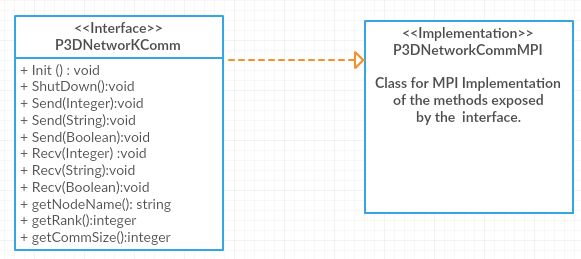
\includegraphics[scale=0.75]{Interface.png}
\caption{Class Diagram for the Interface}
\label{fig:InterfaceDiagram}
\end{figure}


\subsection{How does MS-MPI work internally?}

MPI as mentioned in the earlier sections provides the methods which allow for communication via message passing in a point-to-point communication or collective communication paradigm. MPI specifies a standard on what a message passing interface is supposed to do and not how it is done. The part of how it is done is decided by the implementation. The implementation can provide MPI methods using different underlying protocols and performance of the communication depends on the implementation, the underlying network and type of data communicated. MPI is message oriented protocol meaning that data is sent in distinct packets which are assembled at the receiver whereas a stream oriented protocol will have data sent byte-by-byte i.e. stream of bytes.The size of the data sent determines the way in which the message is sent or received. The underlying message protocol can be {\lq}eager{\rq} or {\lq}rendezvous{\rq} protocol\newline 

\textbf{Eager Message Passing Protocol}- The responsibility of storing the message is done at the receiver's end if no matching receive has been posted by the receiver. The sending process sends the message which is received by the receiving process if the matching receive has been already posted other wise the message is buffered by the receiving process. The sending process sends the message irrespective of whether the receive has been posted or not. It is allows for easy implementation of MPI\_Send and better performance as the send call does not need to block to get an acknowledgment from the receive operation. The problem is that this solution is not scalable and may lead to memory exhaustion if there are large number of messages which need to be buffered at the receiver. Another problem is the extra copy of the buffered message is required at the receiver from the buffered space i.e. the buffer allocated in the kernel space to the receiver's buffer i.e. the buffer allocated  in the receiver process's address space. This also leads to investing CPU cycles for the extra copy to be made.       

\textbf{Rendezvous Message Passing Protocol}- This protocol can be used on top of the eager protocol i.e. when the buffering limit has been reached. There is no underlying assumption made by the sending process that the receiver can allocate the memory and hence need to first signal the receiver process about the incoming message. This signaling is called as {\lq}handshake{\rq}. The format of the message for MPI was introduced in the  section \ref{MSMPI-API}. The Figure \ref{fig:MessageFormat} shows the message format specified by MPI standard \cite{mpiMsgForm}. During the handshake the following actions are performed in the specified order: 

\begin{enumerate}
\item The receiver process first receives the envelope of the message to be sent from the sender.
\item The received envelope is stored by the receiver process if there is no buffer space. 
\item As the buffer space becomes available, receiver process sends an acknowledgment to the sender, indicating that it can receive the message.
\item The sender after receiving the acknowledgment from the receiver, sends the actual payload. 
\item The receiver then receives the message. 
\end{enumerate}   

The protocols fixes the buffer exhaustion issue by not overwhelming the receiver's buffer by actual data rather the receiver needs to just store the envelope of the message which is relatively smaller in size. Therefore makes the receiver process more robust as the receiver does not hang because of buffer overflow. As the messages are received after the acknowledgment by the sender, CPU cycles are saved as the data can directly be copied to the buffer allocated in process's address space. The problem with this protocol is extra messages exchanged during the handshake. 

\begin{figure}[ht!]
\centering
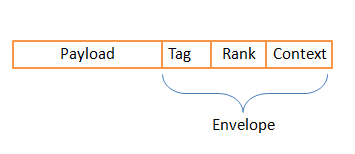
\includegraphics[scale=0.75]{MessageFormat.png}
\caption{Format of MPI Message}
\label{fig:MessageFormat}
\end{figure}

The receive event of a message can either be notified through an interrupt or the receiving process can poll at regular intervals to check if a message has arrived \cite{mpirel}. The interrupt technique works better when the send/receives are asynchronous i.e. they are non-blocking where as polling works well in case of synchronous send/receives i.e. they are blocking. In the polling mode,the receiver process busy waits using the CPU and queries the hardware frequently and manages the messaging by bypassing the OS where as in interrupt mode, the receiving process interacts with the OS which might decide to suspend the process while it is waiting for the message. As the time wasted in the context switch can be significant if the receive event is frequently done as well as OS involvement is generally costly, for better performance reasons the polling method is used by the implementations of MPI specification. \newline

MPI can use TCP/IP as the underlying protocol for message passing in a cluster connected via Infiniband i.e. TCP/IP over Infiniband (IPoIB) or it can use lower level protocols like the OpenFabric protocol or Qlogic Performance Scaled Messaging Protocol or it could as simple as TCP/IP over Ethernet. Microsoft's implementation of MPI-2 specification varies from others such that it uses mechanisms by which the use of TCP/IP can be bypassed. MS-MPI uses Microsoft WinSock Direct Protocol for compatibility over different kinds of Ethernet interconnect and CPU efficiency. The WinSock direct protocol \cite{SDP} uses remote direct memory access i.e. RDMA and thereby bypasses TCP/IP stack as it goes directly to the network interface card allowing for high-speed communication of data. When the TCP/IP stack is bypassed, the overhead occurred due to use of extra CPU cycles and memory bandwidth could be avoided. Winsock Direct Protocol reduces the library overhead and application distribution can scale better even over traditional interconnect networks. Figure \ref{fig:WinsockProto} depicts how the WinSock protocol works \cite{msmpiWinSoc}. \newline

\begin{figure}[ht!]
\centering
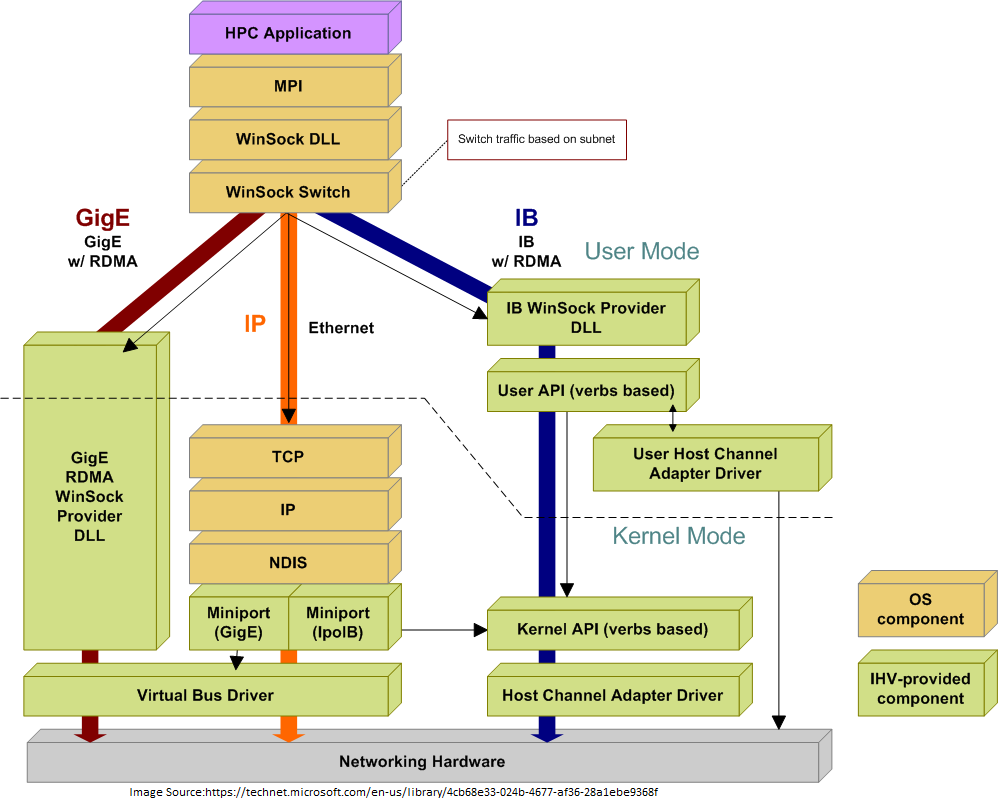
\includegraphics[scale=0.85]{WinSockProtocol.png}
\caption{WinSocket Direct Protocol Behavior}
\label{fig:WinsockProto}
\end{figure}
   
\section{Comparison of MPI to traditional socket programming}

MPI is designed to allow communication amongst HPC (high performance cluster) and preferred choice of programmers over traditional socket programming \cite{mpivssock}. The goal of programming applications to run on HPC is to perform huge and complex computation in a distributed manner if possible. To achieve this goal, programs which perform splitting of huge tasks into smaller sub-tasks and accumulation of partial results to generate final output are written. The logic to perform splitting of tasks, accumulation of results, synchronization and communication if needed among the cluster nodes requires significant programming effort and leads to complicated code. So, it is justified that the developers use libraries which abstract from the underlying complexities of communication but allow to write simple, clean and understandable code. MS-MPI is one such implementation of MPI-2 specification which not only provides decent performance but also lets developers not be bothered about managing the IP addresses, sockets/connection - opening and closing them, and other idiosyncrasies of the underlying network. Simple MPI\_SEND and MPI\_RECV calls do the magic necessary for successful communication. MPI allows to use customized proprietary networks leading to high-throughput and low latency communication. These networks provide abstractions which might not be suitable for socket programming and in-turn lead to lower performance of the application when sockets are used. \newline          

The problem with MPI-2 specification based implementation is lack of robustness when the communication fails amongst the network. There is no standardization of error management and reporting which leads to vague error messages being shown in an event of failure. This is where socket programming might win against MPI as level of robustness provided is pretty standard. Another issue with MS-MPI is that the spawning of the processes and group management is done when the application is launched and dynamic scaling up/down of cluster resources cannot be done at run-time. The cases where the number of sub-tasks are lowers than the configured cluster size needs to be handled by the implementation. So, when the number of print object files in the main configuration is less than the number slave nodes in the cluster, the master needs to drop some of the slaves from the cluster and only wait on {\lq} working nodes{\rq} for partial output. 
	
\section{External Libraries}

Libraries which are developed by external sources are referred to as {\lq}External Libraries{\rq} in the current documentation. The external libraries offer specific functionality which can be used by the applications. Generally the use of such libraries is encouraged as they allow the developer to use the already implemented solution and focus on the in-hand problem statement instead of reinventing the wheel. These external libraries are generally are high-quality as they are mostly rigorously tested and used in different kinds of target applications. The algorithms implemented to perform the task by the libraries provide good efficiency at a low-cost. The probable problem of using an external library is that if there is a bug in the library then all the applications using these library duplicate the bug. \newline

In the implementation of the thesis, the following external libraries are used:    
\begin{enumerate}
\item \textbf{Little Color Management Engine(lcms) Version 2.0}: It is an open source small-footprint color management engine which uses ICC standard (International Color Consortium). It provides numerous APIs which can be used to access (parse, read, write) the ICC profiles, access (read/write) tags and profile structures, create formatters which describe the organization of the bitmap buffers and performing color transformation.  In the implementation of prototype II, the master reads the ICC profile  and sends the byte stream to the slave nodes. The master node uses \textbf{\textit{cmsOpenProfileFromFile}}, \textbf{\textit{cmsSaveProfileToMem}} APIs where as slave nodes use \textit{\textbf{cmsOpenProfileFromMem}} API. The header {\lq}lcms2.h{\rq} should be included to use the mentioned APIs. The syntax and the use of the APIs is described below:

\begin{itemize}
\item \textbf{\textit{cmsOpenProfileFromFile}}- API used to open the profile from the file on the disk \ref{lst:OpenProfileFromFile}.
\item \textbf{\textit{cmsSaveProfileToMem}}- API used to save the profile to the memory block \ref{lst:SaveProfileToMem}. 
\item \textbf{\textit{cmsOpenProfileFromMem}}- API used to open the profile already in the stored in a memory block \ref{lst:OpenProfileFromMem}. 
\end{itemize} 

\item \textbf{RapidJSON}- It is an open-source JSON parser/generator for C++ supporting both SAX/DOM style API. It is not only fast, small and header-only but also is unicode and memory friendly. It provides APIs to parse, read, write/modify and query value from the JSON document. The APIs are used with the \textit{rapid::json } namespace. The following RapidJSON library APIs are used:
\begin{itemize}
\item \textbf{\textit{IsObject}}- Normally a type {\lq}Value{\rq} stores the JSON value and {\lq}Document{\rq}, holds the root Value of the DOM tree. IsObject is an API to check if the root is a DOM object.
\item \textbf{\textit{ParseStream}}- API used to parse the JSON stream from the input.
\item \textbf{\textit{HasMember} and \textit{AddMember}}- APIs used to check if the specified member is present in the object and to add the member to the object respectively. 
\item \textbf{\textit{setters} and \textit{getters}}- APIs used to set \{SetString\} and get a value \{GetArray, GetInt, GetUint, GetString, GetObject\}.
\item \textbf{\textit{Queries for value type}}: IsBool, IsNull, IsNumber, IsString are the APIs which allow to check the type of the value. 
\end{itemize} 
  
\item \textbf{Zlib}- It is a general purpose compression library providing functions to perform compression and decompression of data. The functions provided use in-memory buffers which allows for compressing the whole data at once by using deflation compression methodology. The library also offers functions to perform integrity check on the compressed data and functions to read/write files with gzip format. The following APIs are used for compression/ decompression in the implementation of prototype II where slices are sent and received as stream of bytes.  
\begin{itemize}
\item \textbf{\textit{compress2}}- Compresses the source buffer into the destination buffer \ref{lst:compress2}. The last argument of the API is used to set the compression level which can be Z\_BEST\_SPEED for best speed, Z\_BEST\_COMPRESSION to get the smallest size of compression or Z\_DEFAULT\_COMPRESSION for default compression.
\item \textbf{\textit{Decompression}}- Decompresses the source buffer into the destination buffer \ref{lst:uncompress}. The size of the decompressed data should be communicated to the site where the decompression is performed so that the buffer with appropriate size could be allocated.
\end{itemize}
\end{enumerate}
   
\begin{lstlisting}[language=C++,label={lst:OpenProfileFromFile},caption={Open profile from File}]
cmsBool cmsOpenProfileFromFile(cmsHPROFILE hProfile, void *MemPtr, cmsUInt32Number* BytesNeeded);
\end{lstlisting} 

\begin{lstlisting}[language=C++,label={lst:SaveProfileToMem},caption={Save profile to Memory}]
cmsBool cmsSaveProfileToMem(cmsHPROFILE hProfile, void *MemPtr, cmsUInt32Number* BytesNeeded);
\end{lstlisting} 

\begin{lstlisting}[language=C++,label={lst:OpenProfileFromMem},caption={Open profile from Memory}]
cmsHPROFILE cmsOpenProfileFromMem(const void * MemPtr, cmsUInt32Number dwSize);
\end{lstlisting} 

\begin{lstlisting}[language=C++,label={lst:compress2},caption={API to compress the data}]
int ZEXPORT compress2(Bytef *dest, uLongf *destLen,const Bytef *source, uLong sourceLen, int level);
\end{lstlisting} 

\begin{lstlisting}[language=C++,label={lst:uncompress},caption={API to uncompress the data}]																	
int ZEXPORT uncompress(Bytef *dest, uLongf *destLen, const Bytef *source, uLong sourceLen);															
\end{lstlisting} 																	

\section{Debugging}

During the implementation, there will be many occasions on which it would not be possible understand the reason for the wrong output of the program by just observing the output or log file. Hence, developers perform a multi-step process of identification and isolation of the problem followed by correcting the problem which altogether is called as the debugging process. Microsoft Visual Studio 12 provides an inbuilt debugging tool which comes very handy to debug the application. 
As the application modified through the thesis runs on the cluster, a new challenge of which and how should the instance of the application be debugged had to be addressed. There were two possible solutions- using a remote debugger or use a local debugger by changing the role/rank of the machine in the cluster. \newline

Debugging a parallel application using remote debugger tool can be performed by searching for the process representing the instance of the application running on the node i.e. the remote machine and attaching the process to the visual studio process on the local machine. The debugging process done in this manner is quite slow and might be tricky to debug applications which crash at the very start giving the developer very small time interval to find and attach the process. The advantage is that debugging can be done on the local machine with the local visual studio instance running and hence installation of visual studio on the remote location is not required. \newline

Debugging done by changing the rank of the local machine in the cluster is simple, faster and same as performing local debugging. Depending on the rank, a node acts as the master or a slave and so changing the role of the local machine helps to debug the application behavior for master or slave node. The rank of the local machine can be 0 i.e. master if it is the first value for the -hostname argument of the mpiexec command or \gt 0 i.e. slave node, if it is not the first value for the -hostname argument. As this method was faster, debugging of the distributed cuttlefish application during the implementation was done by using this method. 
 
\section{Project Management}


\newpage
  
\chapter{Results and Analysis}

After the implementation phase of the design discussed in the previous chapter, the next phase involved performing tests to check if the implementation worked. To recapitulate the problem statement intended to be solved through the thesis was to increase the performance of the cuttlefish application by adding more computational capacity and distributing the objects to utilize the added computational power. The first part of the goal was achieved by creating a distributed system of heterogeneous systems as compute nodes connected through the enterprise network. For utilizing the computational capacity added, the application had to be modified to perform distribution of the work items amongst the computes nodes, collect their partial results and use the partial result to generate the final output. The desired result to be achieved through the thesis primarily was less computation time for multiple models as compared to computation time needed by current cuttlefish application and increase resource utilization by making use of the available machines.\newline

\section{Overview of SDLC Testing Phase} \label{SDLCTesting}

In the software development life-cycle, testing phase follows the implementation phase wherein various tests are conducted to verify and validate the implemented software. The result of the testing phase depends highly upon the type of test cases which are run. Testing can be classified into various categories depending on criteria chosen for classification, for example: the methods chosen to conduct tests, levels of testing etc. On the basis of methods used for testing, testing can be performed by manually testing the software or by automating the tests. In manual testing, the tester uses the software as an end-user and makes note of the deviations(if any) seen in the behavior of the system as from the expected. In automated testing, another software or scripts are used to run the various test-cases for the software under consideration. Each of these broadly classified types of testing techniques can consists of unit testing, integration testing, system testing, performance testing, regression testing etc.\newline

Manual testing as stated earlier is done by the tester by running the various use-cases in which an end user might execute the system. Mostly, manual testing is done to verify the system's behavior with respect to the specification which involves unit testing, integration testing. The validation of the implementation is done with respect to satisfying the needs of the customer which generally involves user acceptance tests and usability tests. Automated testing is generally done to perform regression testing where in part of the software under consideration is being fixed for some bug found by verification process, by re-writing a piece of code or introducing the fix by a new piece of code. The goal of regression tests is to ensure that the fixed bug is not leading to newer bugs in the system and thus is done quite frequently i.e. each time a discovered bug is fixed. Automation testing is also used to conduct stress test or performance tests where in the system is subjected to different loads and the behavior is observed with the primary goal to measure the performance or efficiency of the system under varying loads. As automation testing involves using other software or scripts to perform the tests, it cheaper and efficient both in terms of money and time. \newline 

On the basis of level of testing, testing can be done to check the functional or non-functional requirements. Functional requirements cover what the software is intended to do i.e. for a given input, the systems performs the intended task and the results generated by the system are correct. Non-functional requirements from the system involve checking the performance of the system, the resource utilization etc. \textbf{Functional testing} can broken down further into discrete levels as follows: 

\begin{itemize}
\item{\textbf{Unit Testing}}- Generally, it is performed by the developer who is aware about the code and the new modules which are implemented. The unit which is tested is generally doing a particular task / dedicated task and is a smaller portion of the whole code. The goal of the test is to ensure that each unit is performing the functionality it is implemented for. Unit tests generally have quite limited scope as it is not possible to cover all the execution paths of a code and the test data used by the developer is not the same as the test data to be used by the quality assurance team. 
\item{\textbf{Integration Testing}}- As the name suggests, integration testing is done to check if the individual modules tested via unit testing work correctly in unison. The unit testing of lower-level modules can be done first followed by integration tests by combining one or more modules which is called as bottom-up approach. If all the system modules together are tested i.e. the highest-level of module is tested first followed by testing each module individually later, it is called top-down approach.
\item{\textbf{System Testing}}- System testing is generally done by a specialized quality assurance team where in the system is tested as a whole to check if the system meets the quality standards agreed upon. The system is tested in an environment which is very similar to the production environment i.e. the environment where the developed application is going to be deployed.
\item{\textbf{Acceptance Testing}}- One of the most crucial steps of testing, the QA team verifies if the application works correctly for test scenarios which are discussed prior to the implementation by the customer and the development team. These test cases are drawn on the basis of the acceptance criteria for the software. 
\end{itemize}        

\textbf{Non-Functional testing} as mentioned earlier includes testing the non-functional requirements of the software such as the performance of the system, security, ease of use of the system etc. Non-Functional testing can be broken down into following levels: 

\begin{itemize}
\item{\textbf{Performance Testing}}- Performance testing involves exposing the system under consideration to various levels of stress and loads to monitor the behavior of the system. The goal of this type of testing is to identify the performance issues or bottlenecks which could be caused by network delay, large data input size, hitting peak processing capacity etc.  
\item{\textbf{Usability Testing}}- This type of testing involves the checking the ease of use for the software where the possible improvements in the software are noted by observing the users use the software. It involves checking the efficiency of use, learn-ability, error messages seen by the user and satisfaction of the user.
\item{\textbf{Portability Testing}}- If the software is built with multi-platform support, then this type of testing checks the functioning of the software on different platforms. The diversity in the platforms covers checking different operating systems, different underlying architecture or type of network.    
\item{\textbf{Security Testing}}- The intention of security testing is to find any vulnerabilities in the software which would compromise the security guarantees that should be provided by the software. The checks are done to ensure confidentiality, integrity, authentication, availability, authorization, non-repudiation, buffer over-flow vulnerabilities etc. 
\end{itemize} 

\section{Implementation Assessment}

Amongst the types of testing discussed in the Section \ref{SDLCTesting}, the implementation of the thesis was tested by using manual testing during the development and automated testing after the development was done. The manual testing involved running the scenarios to check individual components or parts of the components.  
Following the unit tests, were the tests which involved checking how the components worked together for different scenarios. Some of the manual tests performed are described in Section \ref{ManualTests}. The performance of the distributed cuttlefish is measured through automated testing. The performance tests and results of the tests are discussed in the Section \ref{PerformanceTests}.

\subsection{Manual Tests} \label{ManualTests}

Out of the various test cases which were conducted, the important cases have been documented in this Section which highlight the scenarios testing the components newly introduced for distributed computing. 

\begin{enumerate}
\item{Test-cases specific for Prototype I}: The prototype I tests included testing the \textit{MasterDistributor}, \textit{SlaveReporter} and \textit{MasterMerger} components. 
\begin{itemize}
\item{\textbf{Test-Case for \textit{MasterDistributor} Component}}:

\begin{itemize}
\item{\textbf{Scenario}}- To test if the \textit{MasterDistributor} component generates correct distribution for a given set of input objects and cluster size. The goal is to test the correct calculation of the threshold function, creation of distributed print object list and using the generated list correctly writing the main configuration file for each slave node.  
\item{\textbf{Method}}- Distributed cuttlefish was executed multiple times with varying inputs. The test data for the simplest scenario consisted of 2 head models to be distributed among 3 node cluster with 2 slaves and one master node. Each head was 8cms and the expected balanced distribution of the input would to be generate load of one head model per slave node. The same test case was run repeatedly with varying the number of input objects, different types of input models i.e. varying the test-data and cluster size. 
\item{\textbf{Results}}- As in prototype I, the \textit{MasterDistributor} component generated main configuration file per slave and the output of the current test was verified by checking the number of print objects in the main configuration file for each slave node. Another way to check the threshold calculation was to use simple standard output statements or logging the information in a trace file.
\end{itemize}

\item{\textbf{Test-Case for \textit{SlaveReporter} Component}}: 
\begin{itemize}
\item{\textbf{Scenario}}- The \textit{SlaveReporter} Component generates the output with partial slices, which are written to the disk after serialization and chunk-wise sending the path to the master. To test if the \textit{SlaveReporter} component generates correct partial output and the path sent to the master is the correct location.
\item{\textbf{Method}}- Distributed cuttlefish was executed on the slave node. To check if the serialization of the partial slices happens correctly, the slices are deserialized at the slave and the partial output is written to the disk as images. The part of code implementing the test i.e. deserialization of the slices and generating images of the partial slices is not part of the final code which is used to build the distributed cuttlefish binary but is rather just code to test the scenario. 
\item{\textbf{Results}}- The images of the partial slices generated by the \textit{SlaveReporter} component were thoroughly checked to ensure correct material assignment. Ensuring that the partial slices are correctly serialized helped to narrow down the errors which were encountered in generation of the merged slices.  
\end{itemize}

\item{\textbf{Test-Case for \textit{MasterMerger} Component}}: 
\begin{itemize}
\item{\textbf{Scenario}}- The \textit{MasterMerger} Component generates the output with merged slices, which are written to the disk in a chunk-wise fashion after de-serialization. To test if the \textit{MasterMerger} component generates correct merged output.
\item{\textbf{Method}}- Distributed cuttlefish was executed in the cluster.To check if the de-serialization of the partial slices happens correctly at the master, the de-serialized partial slices are written to the disk as images before writing to the merged full slices. The part of code implementing the test i.e. deserialization of the slices and generating images of the partial slices is not part of the final code which is used to build the distributed cuttlefish binary but is rather just code to test the scenario. 
\item{\textbf{Results}}- The images of the partial slices generated by the \textit{MasterMerger} component were thoroughly checked to ensure correct material assignment. The final output of the \textit{MasterMerger} component i.e. the merged full slices were verified by checking the output of the \textit{SliceDebug} component output. Through this test a bug in the code was detected wherein the empty full slices created before writing the partial slices were not initialized with empty voxel value i.e. no material assigned these voxels, leading to random value assignment to them which lead to incorrect results, i.e. slices had random patches of materials assigned. 
\end{itemize}
\end{itemize}  

\item{\textbf{Test-cases specific for Prototype II}}: The testing of prototype II was done through the test cases for \textit{MasterPJDistributor}, \textit{SlavePJCollector}, \textit{SlaveReporter} and \textit{MasterMerger} 

\begin{itemize}
\item{\textbf{Test-Case for \textit{MasterPJDistributor} Component}}:

\begin{itemize}
\item{\textbf{Scenario}}- To test if the \textit{MasterPJDistributor} component generates correct distribution for a given set of input objects and cluster size. The goal is to test the correct calculation of the threshold function, creation of distributed print object list and using the generated list correctly to generate the print job per slave node.
\item{\textbf{Method}}- Distributed cuttlefish was executed multiple times with varying inputs. The test data for the simplest scenario consisted of 2 head models to be distributed among 3 node cluster with 2 slaves and one master node. Each head was 8cms and the expected balanced distribution of the input would to be generate load of one head model per slave node. The same test case was run repeatedly with varying the number of input objects, different types of input models i.e. varying the test-data and cluster size. 
\item{\textbf{Results}}- As in prototype II, the \textit{MasterPJDistributor} component generated print job per slave and the output of the current test was verified by debugging the number of print objects in the print job for each slave node. Another way to check the threshold calculation was to use simple standard output statements or logging the information in a trace file. Through this test, a bug in the code which led to incorrect threshold calculation was caught. The incorrect threshold calculation lead incorrect number of print objects in the print jobs leading to one of the computes nodes being overloaded. Another bug related to placement of the print objects in the print bed was discovered as well, where in the print jobs sent to the slaves had print objects with the transformation created by the print job organizer at the master. This lead to generation of partial slices with the print objects placed at some displacement from the origin at the slave. This bug was later fix by changing the behavior of the \textit{MasterMerger} component for prototype II.
\end{itemize}

\item{\textbf{Test-Case for \textit{SlavePJCollector} Component}}:

\begin{itemize}
\item{\textbf{Scenario}}- To test if the \textit{SlavePJCollector} component receives correct input from the master. The goal is to test if the \textit{SlavePJCollector} component correctly receives the serialized print job, deserializes the print job and loads the texture information to the GPU memory after receiving it from the master and deserializing the received texture data.
\item{\textbf{Method}}- Distributed cuttlefish was executed multiple times on the slave node with varying number of input models at the master.
\item{\textbf{Results}}- In the prototype II, the \textit{SlavePJCollector} component receives the serialized print job from the master. The size of the serialized data was cross-examined with the size of data sent at the master node. After deserializing the print job, the number of print objects contained in the print job was checked through debugging the component. To check if the texture data was received and deserialized correctly, the deserialized data was written to an image on the disk. Through this test, a bug in the format in which the texture data was uploaded to the GPU memory at the slave node was found. The texture data is in RGBA format and is linearized at the master node before uploading the data to master node GPU. When the texture data is communicated to the slave, the load operation should not perform the linearization again and instead load the data directly to the GPU memory.
\end{itemize}
\end{itemize} 

\item{\textbf{Test-Cases Common for Prototype I and Prototype II}}:
There are some corner cases which had to be checked for both the prototypes. These scenarios and the tests performed to check how the system handles these scenarios are described as follows:

\begin{itemize}
\item{\textbf{Corner Case I}- Size of input objects < number of slave nodes }
\begin{itemize}
\item{\textbf{Scenario}}- To test the behavior of distributed cuttlefish when the number of input objects submitted to the master node is smaller than the cluster size i.e. number of print objects in the main configuration file are less than the number of slave nodes.
\item{\textbf{Method}}- Distributed cuttlefish was executed with submitted main configuration file consisting of less number print objects in comparison to the number of nodes given to mpiexec command, i.e.  cluster size is number of print objects plus 2 (as master node does not act as a slave node)
\item{\textbf{Results}}- When the number of print objects is less than the number of available slave nodes, some of the slave nodes get empty input. At the master, the \textit{MasterMerger} component is notified the number of slaves nodes doing the actual work so as to ensure that the \textit{MasterMerger} component waits to receive the partial slices only from these many slave nodes. For prototype I, the empty work item to the {\lq}dropped{\rq} slaves is given by writing a main configuration file without any print object files. Through this test case, it was discovered that the cuttlefish application did not handle empty input case and crashed. So to handle the empty input, there were some modifications introduced in the application. For Prototype II, the empty input the {\lq}dropped{\rq} slaves is given by sending a print job without any print objects. The {\lq}dropped{\rq} slaves do execute the whole pipeline once with null input and wait for the other slaves doing the work to finish while they execute MPI\_Barrier call.     
\end{itemize}
\item{\textbf{Corner Case II}- Size of input objects = 1}
\begin{itemize}
\item{\textbf{Scenario}}- To test the behavior of distributed cuttlefish when only one print object is submitted to the master node, i.e.the main configuration file contains only one print object file.
\item{\textbf{Method}}- Distributed cuttlefish was executed with submitted main configuration file consisting of 1 print object.
\item{\textbf{Results}}- Irrespective of the number of slave nodes in the cluster, as there is only one print object provided as input to the distributed cuttlefish, there is no need to calculate the threshold to perform the distribution. So, the slave node with rank 1 i.e. the first slave node in the cluster gets the print object and rest of the slave nodes (if any depending on the number of hosts set in the mpiexec command) are {\lq}dropped{\rq} and the behavior of the system is similar to the behavior discussed in the above test-case.
\end{itemize}

\item{\textbf{Corner Case III}- No input given to the distributed cuttlefish}
\begin{itemize}
\item{\textbf{Scenario}}- To test the behavior of distributed cuttlefish when input of size is 0.
\item{\textbf{Method}}- Distributed cuttlefish was executed with submitted main configuration file consisting of 0 print objects.
\item{\textbf{Results}}- When the input size is 0, for prototype II, the \textit{MasterPJDistributor} component gets an empty print job from the \textit{PrintJobOrganizer} component. The \textit{MasterPJDistributor} component informs the \textit{MasterMerger} component that all the slave nodes are dropped and it should not wait for any partial output from the slave nodes. For prototype I, all the slave nodes receive empty configuration files and the master behaves the same as in prototype II. 
\end{itemize}
\end{itemize}
\end{enumerate}

 
\section{Results} \label{PerformanceTests}

The performance testing is done through automation of the test-cases. To perform automated testing, either another software is used to run the software under test or scripts are written to perform the testing. For testing the distributed cuttlefish, batch scripts were written and executed to perform the tests. For each test case, the test-data was created along with the script and the task was scheduled using the windows task scheduler. The performance tests were conducted to check the computation speed-up and efficiency achieved by distributed computing. The Section \ref{DistvsNonDist} explains the terms computational speed-up and efficiency in parallel computing followed by the test case used to find the speed-up and observed result. The Section \ref{ProtoComp} details the comparison of the two prototypes developed in terms of computation speed-up, communication overhead and how well the prototypes scale for a given work load.

\subsection{Comparison of distributed vs non-distributed cuttlefish performance} \label{DistvsNonDist}

Speed-up is one of the most common metric used to measure performance of a parallel processing and is defined as the gain by parallel computation in terms of performance in comparison to the sequential computation. \textit{Absolute speed-up} calculation can be done by considering how fast the computation can be performed by using N processors in comparison to best sequential algorithm performance on a single processor \cite{Speedup}. \textit{Relative speed-up }is defined as the ratio of performance of parallel algorithm on one processor to the performance of same on N processors. \textit{Relative speed-up} is used to compare how well the algorithm performs when the number of processors is scaled up \cite{Speedup}. To do performance evaluation for distributed cuttlefish, we use the absolute speed-up definition and Equation \ref{eq:speed-up} to calculate the speed-up, where N is number of processors, \begin{math} T_{s} \end{math} - is the execution time of non-distributed cuttlefish for the given work load, \begin{math} T_{N}\end{math}- is the execution time of distributed cuttlefish for the same work load.

\begin{equation}
\label{eq:speed-up}
\begin{aligned}
S_{N} = T_{s}/T_{N}
\end{aligned}
\end{equation}

Using the Equation \ref{eq:speed-up}, the speed-up can be classified as either linear speed-up, sub-linear speed-up or super-linear speed-up. Linear speed-up is observed when \begin{math}S_{N}=N \end{math} i.e. speed-up is equal to the number of processors. Sub-linear speed-up is when the speed-up is lesser than number of processors where are super-linear speed up is when the speed-up gained is larger than the number of processors. Some of the reasons why super-linear speed-up is possible are higher cache hit rate, better resource utilization, lower network latency for small-sized messages communication. The Figure summarizes the three types of speed-up observed. \newline 

\begin{figure}[t]
\centering
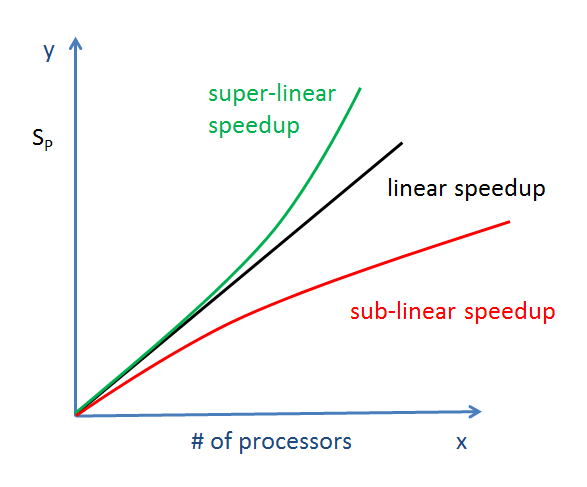
\includegraphics[scale=0.8]{TypesOfSpeedUp.PNG}
\caption{Speed-Up Types}
\label{fig:TypesOfSpeedUp}
\end{figure}

Efficiency is defined as a ratio of speed-up gained for \textit{N} processors to the number of processors. The Equation \ref{eq:eff} is used to calculate the efficiency.

\begin{equation}
\label{eq:eff}
\begin{aligned}
E_{N} = S_{N}/N
\end{aligned}
\end{equation}

\subsubsection{Distributed Cuttlefish Prototype I vs Non-Distributed Cuttlefish}

To check the speed-up gained by using the Distributed Cuttlefish Prototype I, the application was run with different work-loads and comparison between the execution times for both Distributed Cuttlefish Prototype I and Non-Distributed Cuttlefish application was drawn.

\begin{enumerate}
\item{\textbf{Scenario}}- To test the computational speed-up gained by distributed cuttlefish prototype I in comparison to non-distributed cuttlefish for input consisting of same models.
\begin{itemize}
\item{\textbf{Test-Case and Test-Data Description}}- The test case was executed 5 times for each test-data. The cluster was composed of 3 nodes where in one node was the master and remaining two were compute nodes. The cluster nodes were heterogeneous in terms of the number of cores, CPU speed and RAM capacity. The test-data included multiple head models of size 8cms. The number of head models was increased by factor of 2 for each following test-case, i.e. starting with 2 head models the number was increased to 10 head models for the 5 test-cases, with each test-case executed 5 times to enable collection of the average execution times. The speed-up for each test case was calculated using the average execution time for distributed cuttlefish and non-distributed cuttlefish for a given test-data i.e. given work-load. The non-distributed cuttlefish application was executed on the slowest node of the cluster as the slowest node in the cluster would impact the execution time of the distributed version. 
\item{\textbf{Results}}- To elaborate on the amount of work to be done, each 8 cm head model consists of 777 slices with each slice having the width-946 units (8.00 cm)and height-303 units (5.12 cm). The total number of voxels for each model is calculated using the Equation \ref{eq:NumVoxel} where, \begin{math} T_{NumVoxels} \end{math} is the total number of voxels for a given model, width (W), height(H), length (L) and voxel dimensions (voxDims). For each head model used in the test data, the total number of voxels to be processed is \begin{math} 2.17 \times 10^{8} \end{math}. Each voxel can be assigned values denoting the materials and a null material value depending upon the printer specification provided. For current test case, the materials provided in the printer specification are VeroCyan, VeroWhite, VeroMagenta, VeroYellow, VeroBlack and EMPTY\_VOXEL as null material . For each material there is a bitmap generated denoting the voxels which are assigned that particular material in the slice. Figure \ref{fig:SliceOutput} shows the material assignment generated for 108th slice of a single head model. The Table \ref{protoIvsND} summarizes the execution times for distributed cuttlefish with prototype I and non-distributed cuttlefish along with the speed-up.  
\item{\textbf{Observation}}- The number of slave nodes is constant throughout the test-cases i.e. 2 slave nodes and the work-load provided to the system is increased for every test-case. The speed-up is calculated as per the Equation \ref{eq:speed-up} and increases with the increase in work-load in comparison to the non-distributed cuttlefish performance. The Figure \ref{fig:ProtoISpeedupVsNumModels} depicts the scaling of the speed-up with increase in work load i.e number of models. The Figure \ref{fig:ProtoISpeedupVsNumModels}shows some interesting results, the speed-up seen is linear with increase in work-load until it reaches a point where in for a given cluster size increase in the load does not provide linear increase in speed-up although the distributed cuttlefish prototype I performs better than non-distributed version. This is proved by calculating the efficiency using the Equation \ref{eq:eff} and by seeing the trend depicted in the Figure \ref{fig:EfficiencyVsNumModels}. 
\end{itemize}

\item{\textbf{Scenario}}- To test the computational speed-up gained by distributed cuttlefish prototype I in comparison to non-distributed cuttlefish for input consisting of different models.
\begin{itemize}
\item{\textbf{Test-Case and Test-Data Description}}- The test case was executed 5 times for each test-data. The cluster was composed of 3 nodes where in one node was the master and remaining two were compute nodes. The cluster nodes were heterogeneous in terms of the number of cores, CPU speed and RAM capacity. The test-data included multiple head and dame models of size 8 cm. The number of models was increased by factor of 2 for each following test-case, i.e. starting with 1 head model and 1 dame model, the number was increased to 5 head and dame models each, for the 5 test-cases, with each test-case executed 5 times to enable collection of the average execution times. The speed-up for each test case was calculated using the average execution time for distributed cuttlefish and non-distributed cuttlefish for a given test-data i.e. given work-load. The non-distributed cuttlefish application was executed on the slowest node of the cluster as the slowest node in the cluster would impact the execution time of the distributed version. 
\item{\textbf{Results}}- To elaborate on the amount of work to be done, each 8cms head model consists of 777 slices, with each slice having the width-946 units (8.00 cm)and height-303 units (5.12 cm). The total number of voxels for each model is calculated using the following Equation \ref{eq:NumVoxel} where, \begin{math} T_{NumVoxels} \end{math} is the total number of voxels for a given model, width (W), height(H), length (L) and voxel dimensions (voxDims). For each head model used in the test data, the total number of voxels to be processed is \begin{math} 2.17 \times 10^{8} \end{math}. Each 8 cm dame model consists of 605 slices, with each slice having the width-946 units (8.00 cm)and height-194 units (3.27035 cm). The total number of voxels for the dame model calculated using the Equation \ref{eq:NumVoxel} is  \begin{math} 1.09495848 \times 10^{8} \end{math}. Each voxel can be assigned values denoting the materials and a null material value depending upon the printer specification provided. For current test case, the materials provided in the printer specification are VeroCyan, VeroWhite, VeroMagenta, VeroYellow, VeroBlack and EMPTY\_VOXEL as null material . For each material there is a bitmap generated denoting the voxels which are assigned that particular material in the slice. The Table \ref{protoIvsNDDiffModel} summarizes the execution times for distributed cuttlefish with prototype I and non-distributed cuttlefish along with the speed-up for input consisting of different models.  
\item{\textbf{Observation}}-  The number of slave nodes is constant throughout the test-cases i.e. 2 slave nodes and the work-load provided to the system is increased for every test-case. The speed-up is calculated as per the Equation \ref{eq:speed-up} and increases with the increase in work-load in comparison to the non-distributed cuttlefish performance. Although, the speed-up achieved for a given number of models with input consisting of only head models was marginally more than the speed-up achieved when distributed cuttlefish was executed with equal number of models with input consisting of different models. The Figure \ref{fig:SpeedUp-ProtoIDiffModelsVsNumModels} depicts the scaling of the speed-up with increase in work load i.e number of models. Unlike the plot seen in Figure \ref{fig:ProtoISpeedupVsNumModels}, the speed-up increases with increase in the work-load and there is no drop in the speed-up.This is proved by calculating the efficiency using the Equation \ref{eq:eff} and by seeing the trend depicted in the Figure \ref{ProtoIDiffModelsVsNumModels}. 
\end{itemize}
\end{enumerate}

\begin{table}[]
\centering
\caption{Speed-Up \& Efficiency: Distributed Cuttlefish Prototype I vs Non-Distributed Cuttlefish For Same Models}
\label{protoIvsND}
\begin{tabular}{|c|l|l|l|c|}
\hline
\textbf{\begin{tabular}[c]{@{}c@{}}Number of \\ Head Models\\ 8cms\\ (Resolution:\\ 300 X 150 X 470)\end{tabular}} & \multicolumn{1}{c|}{\textbf{\begin{tabular}[c]{@{}c@{}}Total Execution Time (in Secs)\\  for Distributed \\ Cuttlefish Prototype I\\ (Cluster Size- 3)\end{tabular}}} & \multicolumn{1}{c|}{\textbf{\begin{tabular}[c]{@{}c@{}}Total Execution Time (in Secs) \\ for Non-Distributed\\ Cuttlefish\end{tabular}}} & \multicolumn{1}{c|}{\textbf{Speed-Up}} & \textbf{Efficiency} \\ \hline
2                                                                                                                  & 173.3568                                                                                                                                                    & 357.3552                                                                                                                       & 2.0614652                              & 0.6871551           \\ \hline
4                                                                                                                  & 363.3992                                                                                                                                                    & 920.566                                                                                                                        & 2.5332101                              & 0.8444034           \\ \hline
6                                                                                                                  & 585.3218                                                                                                                                                    & 1651.1775                                                                                                                      & 2.8209769                              & 0.9403256           \\ \hline
8                                                                                                                  & 836.2334                                                                                                                                                    & 4071.576                                                                                                                       & 4.8672945                              & 1.6224315           \\ \hline
10                                                                                                                 & 1130.514                                                                                                                                                    & 4790.198                                                                                                                       & 4.2371859                              & 1.4123953           \\ \hline
\end{tabular}
\end{table}


\begin{table}[]
\centering
\caption{Speed-Up \& Efficiency: Distributed Cuttlefish Prototype I vs Non-Distributed Cuttlefish For Different Models}
\label{protoIvsNDDiffModel}
\begin{tabular}{|c|l|l|l|c|}
\hline
\textbf{\begin{tabular}[c]{@{}c@{}}Number of \\ Head \& Dame\\  Models -8 cm\\ (Resolution:\\ 300 X 150 X 470)\end{tabular}} & \multicolumn{1}{c|}{\textbf{\begin{tabular}[c]{@{}c@{}}Total Execution Time \\ (in secs)\\  for Distributed \\ Cuttlefish Prototype I\\ (Cluster Size- 3)\end{tabular}}} & \multicolumn{1}{c|}{\textbf{\begin{tabular}[c]{@{}c@{}}Total Execution Time\\ (in secs) \\ for Non-Distributed\\ Cuttlefish\end{tabular}}} & \multicolumn{1}{c|}{\textbf{Speed-Up}} & \textbf{Efficiency} \\ \hline
2                                                                                                                            & 184.25                                                                                                                                                                   & 243.94                                                                                                                                     & 1.323962008                            & 0.441320669         \\ \hline
4                                                                                                                            & 315.342                                                                                                                                                                  & 635.524                                                                                                                                    & 2.015348415                            & 0.671782805         \\ \hline
6                                                                                                                            & 563.3                                                                                                                                                                    & 1171.32                                                                                                                                    & 2.079389313                            & 0.693129771         \\ \hline
8                                                                                                                            & 685.21                                                                                                                                                                   & 1890.706                                                                                                                                   & 2.759308825                            & 0.919769608         \\ \hline
10                                                                                                                           & 988.708                                                                                                                                                                  & 4793.47                                                                                                                                    & 4.848216056                            & 1.616072019         \\ \hline
\end{tabular}
\end{table}

\begin{figure}[t]
\centering
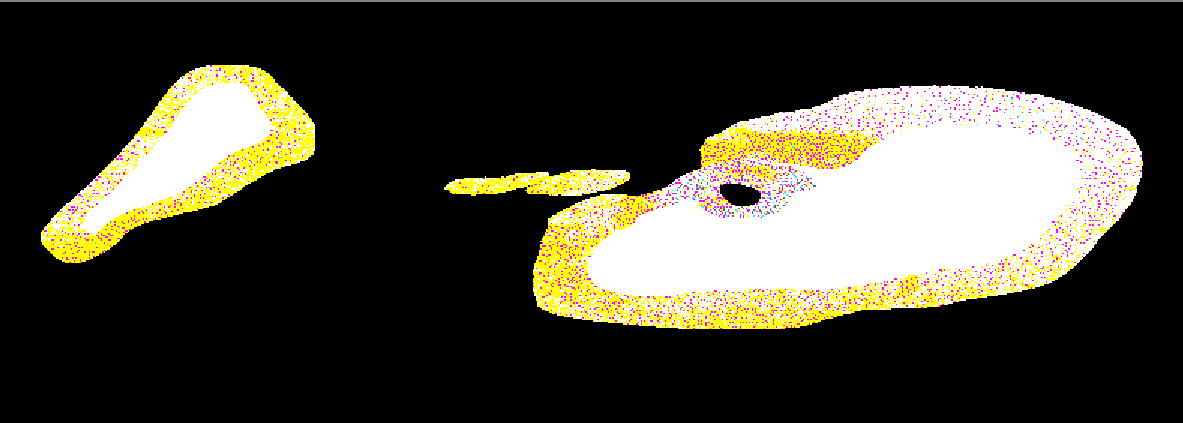
\includegraphics[scale=0.5]{SliceOutput.PNG}
\caption{Material Assignment for Single Slice}
\label{fig:SliceOutput}
\end{figure}

\begin{figure}
\centering

\begin{subfigure}[a]
\centering
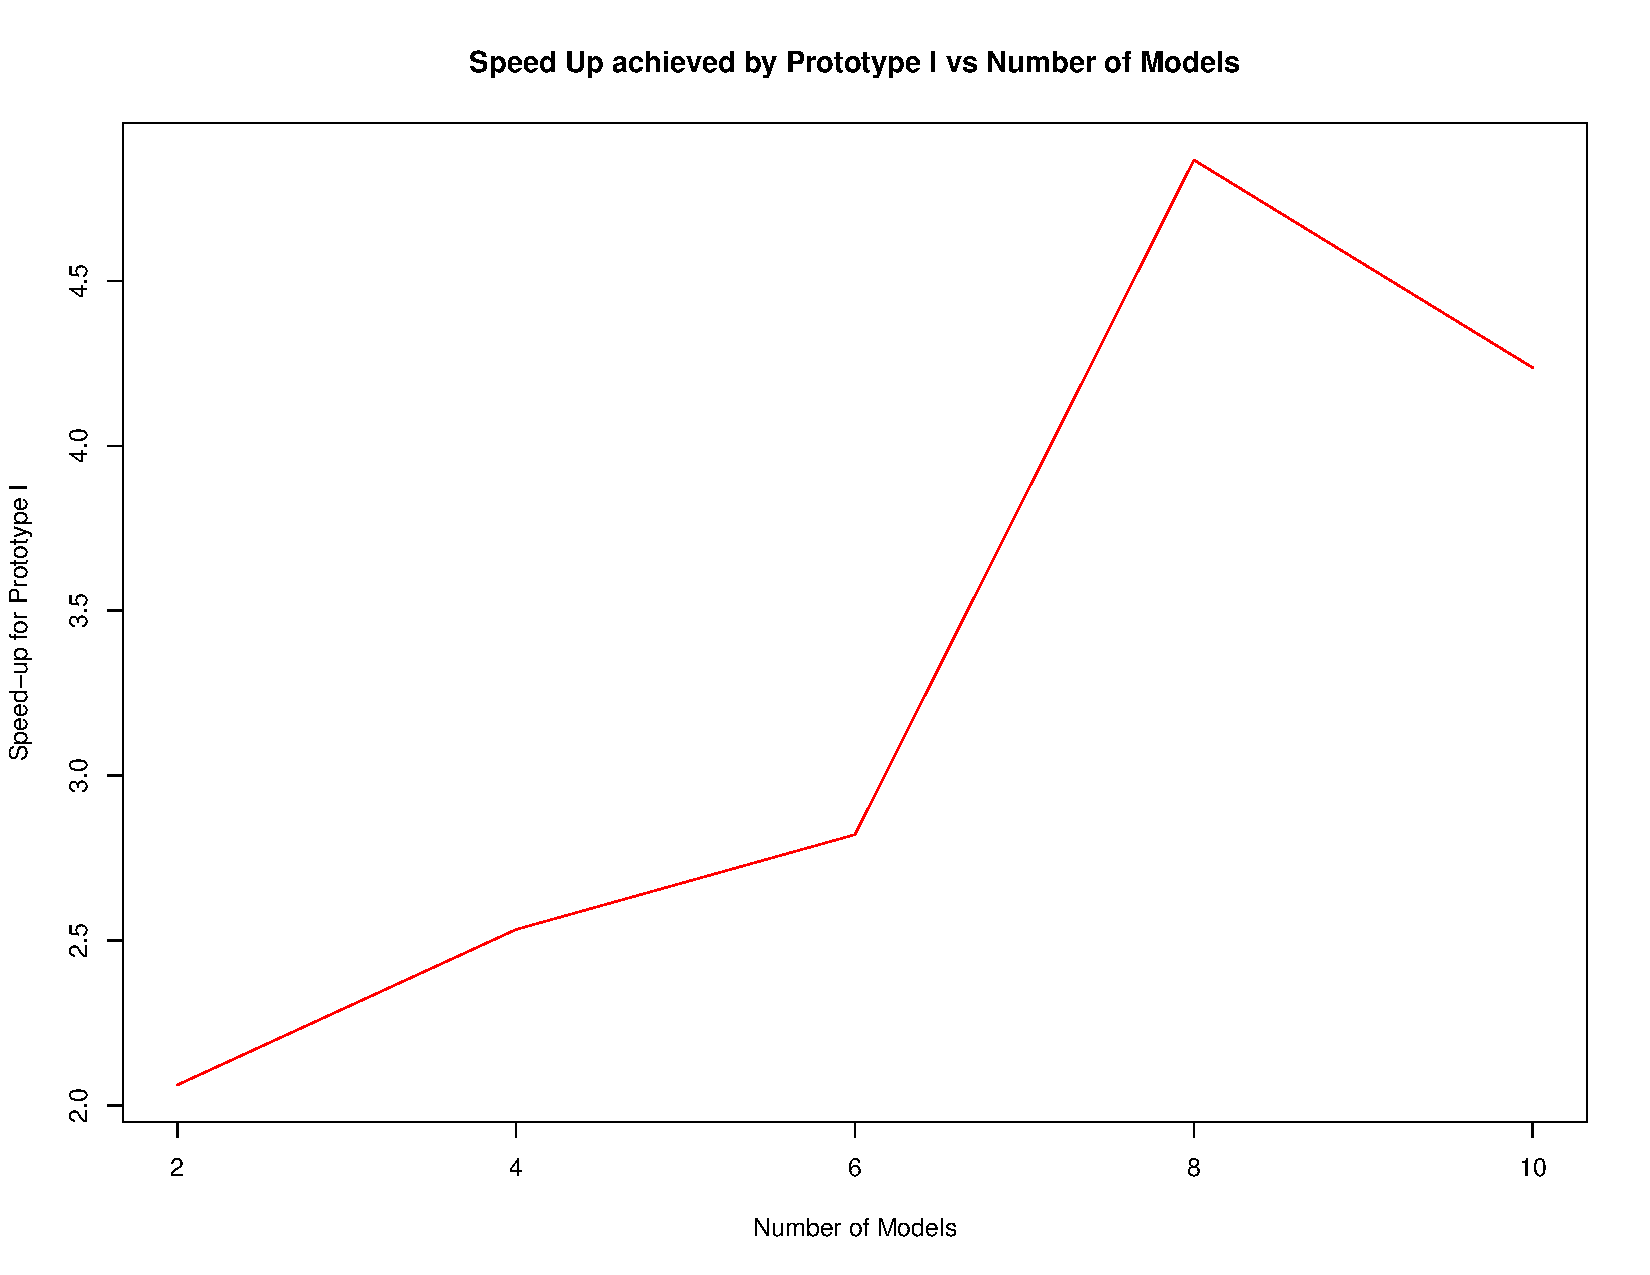
\includegraphics[scale=0.5]{ProtoISpeedupVsNumModels.pdf}
\caption{Speed-up Vs Number of Models}
\label{fig:ProtoISpeedupVsNumModels}
\end{subfigure}
\begin{subfigure}[b]
\centering
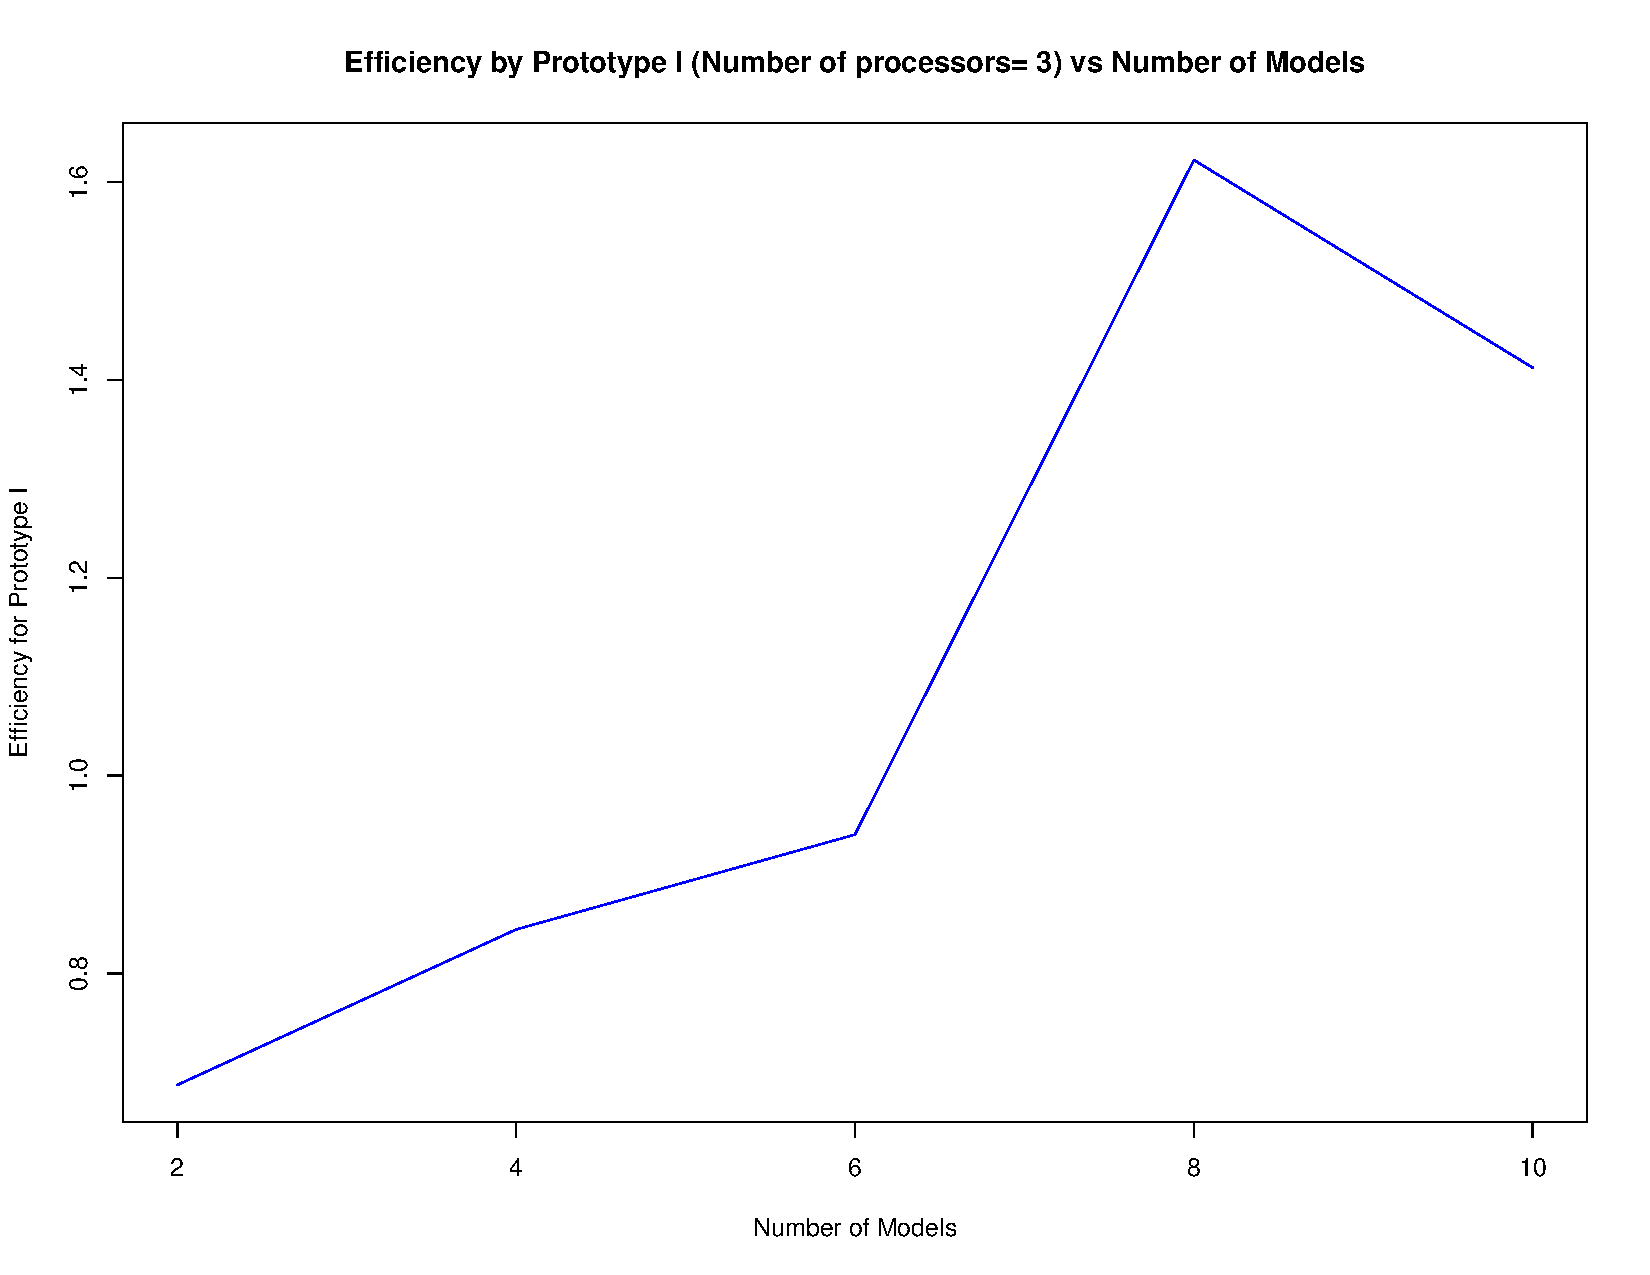
\includegraphics[scale=0.5]{EfficiencyPrototIvsNumModels.pdf}
\caption{Efficiency Vs Number of Models}
\label{fig:EfficiencyVsNumModels}
\end{subfigure}
\end{figure}


\begin{figure}
\centering
\begin{subfigure}[a]
\centering
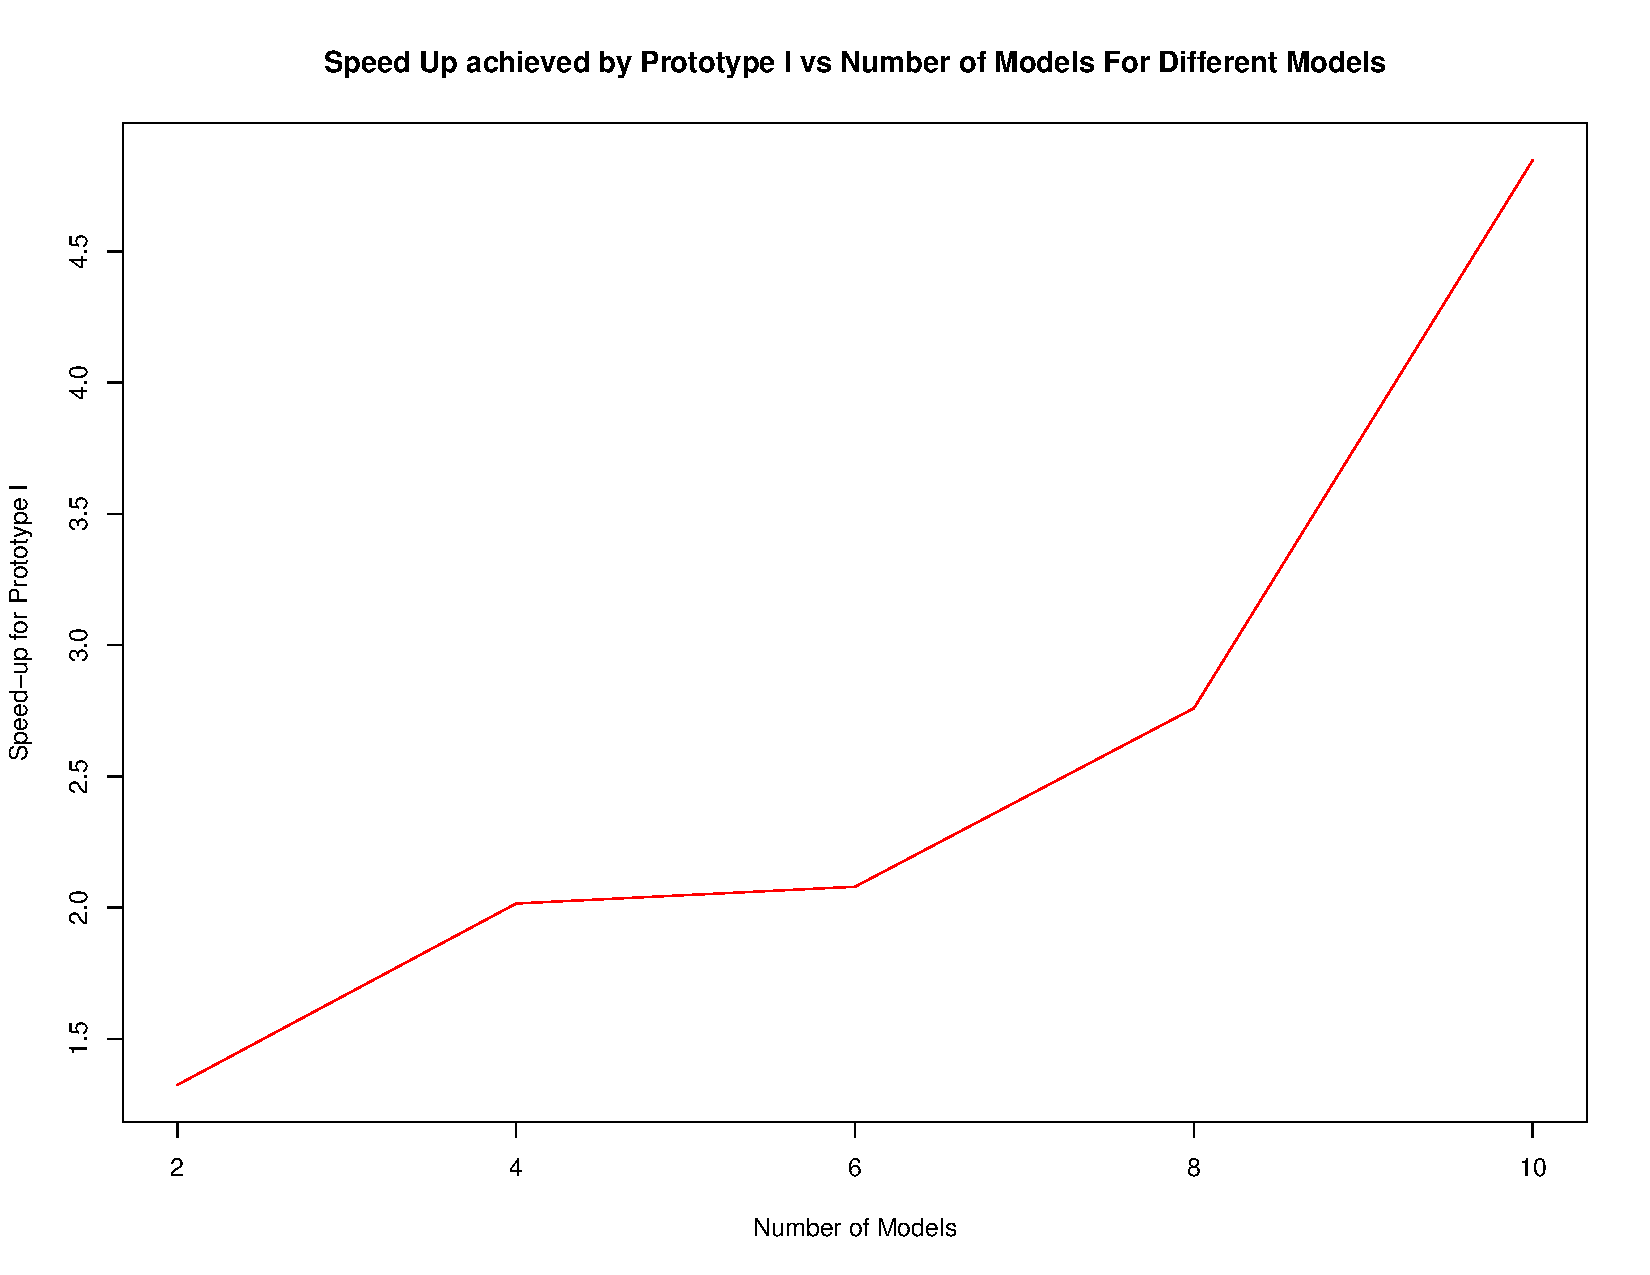
\includegraphics[scale=0.5]{SpeedUp-ProtoIDiffModelsVsNumModels.pdf}
\caption{Speed-up Vs Number of Models}
\label{fig:SpeedUp-ProtoIDiffModelsVsNumModels}
\end{subfigure}
\begin{subfigure}[b]
\centering
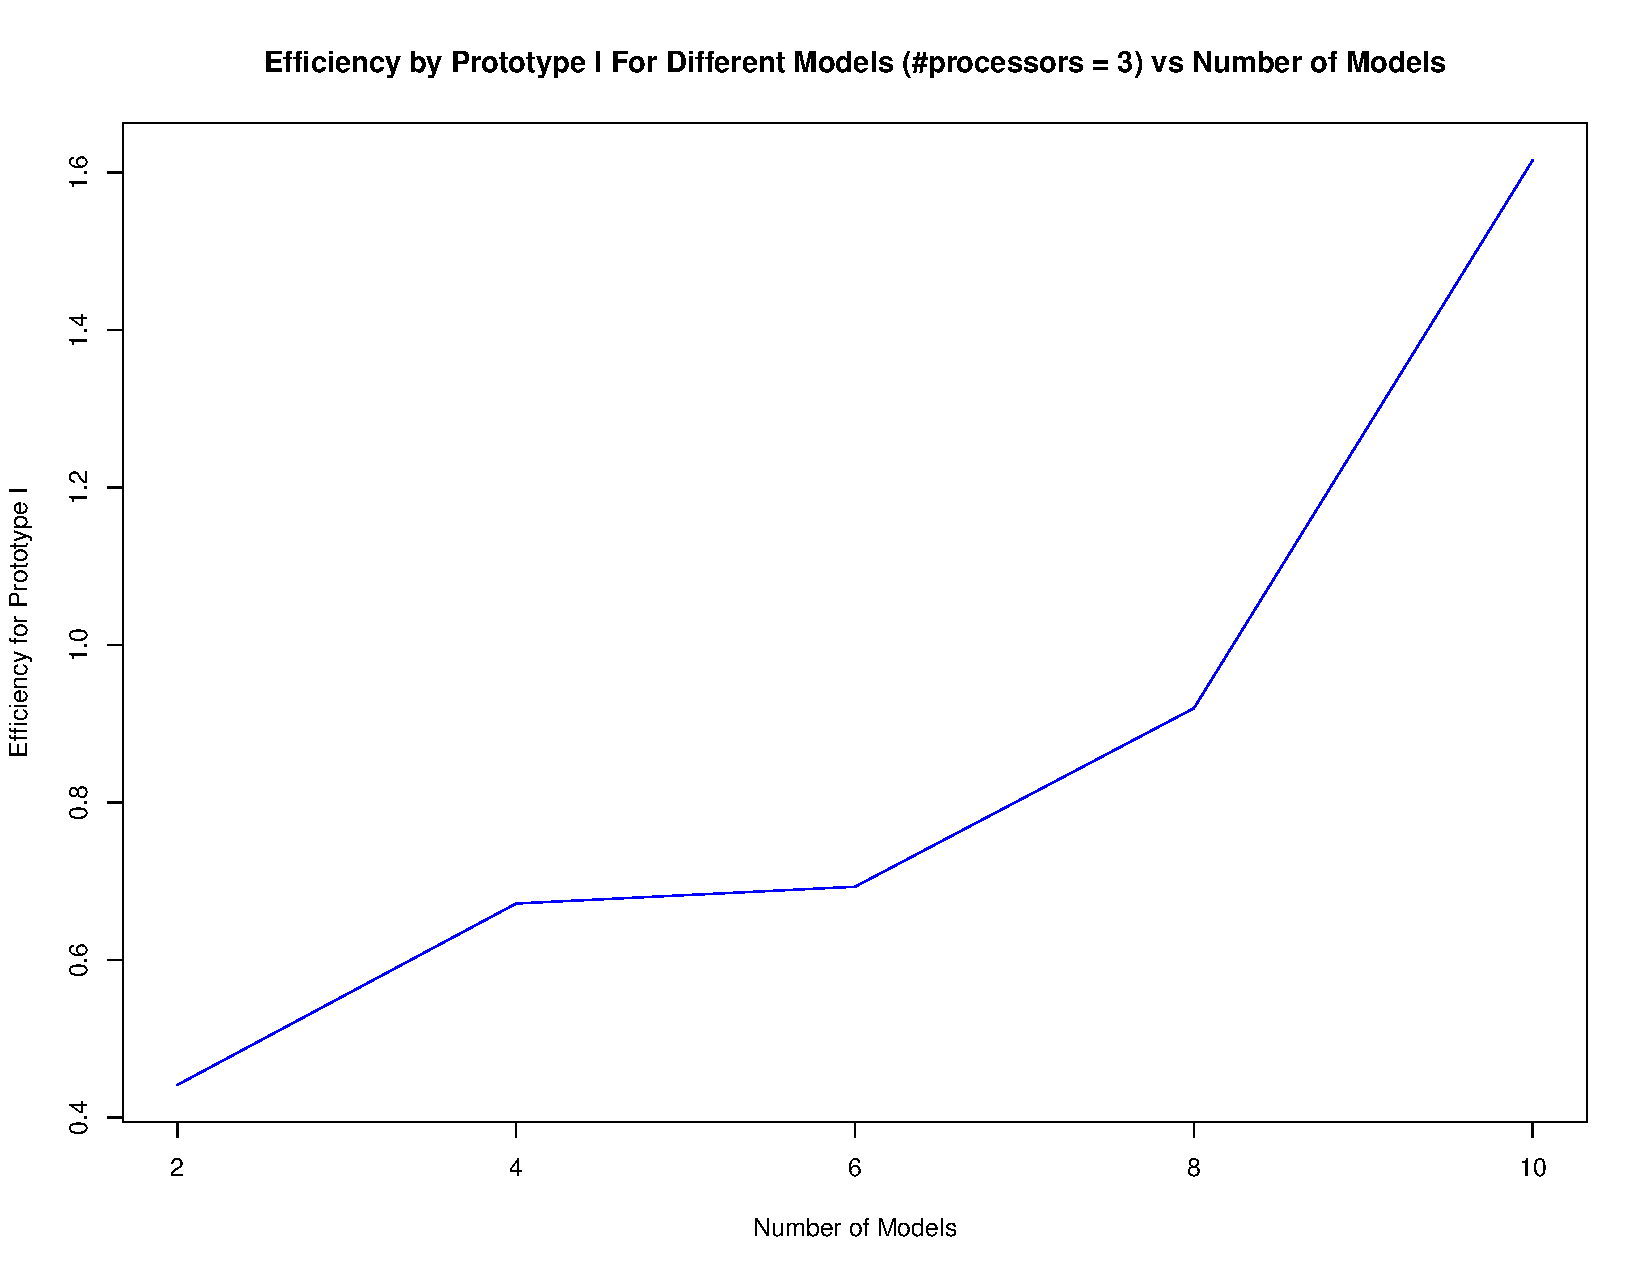
\includegraphics[scale=0.5]{Effi-ProtoIDiffModelsVsNumModels.pdf}
\caption{Efficiency Vs Number of Models}
\label{ProtoIDiffModelsVsNumModels}
\end{subfigure}
\end{figure}


\begin{equation}
\label{eq:NumVoxel}
\begin{aligned}
T_{NumVoxels} = (W\div voxDims.y) \times (L\div voxDims.x) \times (H \div voxDims.z)
\end{aligned}
\end{equation}


\subsubsection{Distributed Cuttlefish Prototype II vs Non-Distributed Cuttlefish}
To check the speed-up gained by using the Distributed Cuttlefish Prototype II, the application was run with different work-loads and comparison between the execution times for both Distributed Cuttlefish Prototype I and Non-Distributed Cuttlefish application was drawn.

\begin{enumerate}
\item{\textbf{Scenario}}- To test the computational speed-up gained by distributed cuttlefish prototype II in comparison to non-distributed cuttlefish for input consisting of same models.
\begin{itemize}
\item{\textbf{Test-Case and Test-Data Description}}- The test-case and the test-data used here is exactly same as the test-case and test-data of Scenario I of Prototype I testing.
\item{\textbf{Results}}- The amount of work done by the nodes remains same as described in Scenario I of Prototype I testing. The Table \ref{ProtoIISameModelsVsND} summarizes the execution time for the test case for prototype II.
\item{\textbf{Observation}}- 
\end{itemize}

\item{\textbf{Scenario}}- To test the computational speed-up gained by distributed cuttlefish prototype II in comparison to non-distributed cuttlefish for input consisting of different models.
\begin{itemize}
\item{\textbf{Test-Case and Test-Data Description}}- 
\item{\textbf{Results}}- 
\item{\textbf{Observation}}-  
\end{itemize}
\end{enumerate}


\begin{table}[]
\centering
\caption{Speed-Up \& Efficiency: Distributed Cuttlefish Prototype II vs Non-Distributed Cuttlefish for Same Models  }
\label{ProtoIISameModelsVsND}
\begin{tabular}{|c|l|l|l|c|}
\hline
\textbf{\begin{tabular}[c]{@{}c@{}}Number of \\ Head \\  Models -8 cm\\ (Resolution:\\ 300 X 150 X 470)\end{tabular}} & \multicolumn{1}{c|}{\textbf{\begin{tabular}[c]{@{}c@{}}Total Execution Time \\ (in secs)\\  for Distributed \\ Cuttlefish Prototype II\\ (Cluster Size- 3)\end{tabular}}} & \multicolumn{1}{c|}{\textbf{\begin{tabular}[c]{@{}c@{}}Total Execution Time\\ (in secs) \\ for Non-Distributed\\ Cuttlefish\end{tabular}}} & \multicolumn{1}{c|}{\textbf{Speed-Up}} & \textbf{Efficiency} \\ \hline
2                                                                                                                     & 135.49                                                                                                                                                                    & 357.355                                                                                                                                    & 2.637501                               & 0.879167            \\ \hline
4                                                                                                                     & 345.342                                                                                                                                                                   & 920.566                                                                                                                                    & 2.665665                               & 0.888555            \\ \hline
6                                                                                                                     & 594.3004                                                                                                                                                                  & 1651.177                                                                                                                                   & 2.778354                               & 0.926118            \\ \hline
8                                                                                                                     & 1534.654                                                                                                                                                                  & 4071.56                                                                                                                                    & 2.65308                                & 0.88436             \\ \hline
10                                                                                                                    & 1832.356                                                                                                                                                                  & 4790.198                                                                                                                                   & 2.614229                               & 0.87141             \\ \hline
\end{tabular}
\end{table}


\subsection{Comparison of Distributed Cuttlefish prototypes} \label{ProtoComp}


  
\newpage
	
\newpage   
\chapter{Conclusion and Future Work}

With research fields like 3d Printing reaching new horizons, it is possible to print high-fidelity print objects due to the features offered by the new generation 3D Printers for high-resolution and multi-material prints. One of the known drawbacks of 3D Printing is that it is slow and mass production of small objects takes too much time making it is costly, as the speed at which the printing can happen is strongly influenced by the material used for printing. Printing these objects economically to look as close as possible to the real-world objects requires a lot processing to be done on the digital input given to the software which generates the information that drives the 3D Printers. Currently Cuttlefish can print multiple objects at the same time reducing the over-all production time for the prints. Although, cuttlefish is capable of performing the computation to enable multiple prints at the same time, it is limited by the machine capacity i.e. the resources offered by the single machine on which the application runs. \newline
To remove system resources as the limitation to perform large scale computation, distributed version of the cuttlefish printer driver was developed through the thesis to allow use of available resources by running the application on the cluster of machines. Two prototypes of the distributed cuttlefish version were implemented using the classic master-slave parallel processing pattern. The difference between the two implemented prototype was the form in which the input was given to the slaves and partial output communication from the slaves to the master. In Prototype I, the communication of the workload from the master node to the slave nodes was done by writing a configuration file per slave node and communicating the file path to the slave node. In Prototype II, the communication of the workload from the master to slaves was in form of stream of bytes consisting of serialized print job per slave node. The partial output communicated by the slaves to the master was writing the serialized partial slices to the disk in Prototype I whereas in Prototype II the serialized slices were compressed and then sent as stream of bytes. The goal of implementing Prototype II was to enable distributed cuttlefish to execute even without a networked file system.\newline 
The distributed system consisted of cluster of heterogeneous processors connected via enterprise network with access to a networked file system. MPI was used to implement the communication between the cluster nodes. Manual testing of the two prototypes was done to check if the application ran as expected for discussed scenarios and automated testing of the two prototypes was done to measure the performance of the application for varying workload and cluster size. Both Prototype I and Prototype II performed better than Non-distributed Cuttlefish for varying number and types of models. The speed-up gained by both the prototypes was at-least linear and in some cases super-linear. One of the possible reasons for super-linear speed up is the cache hit rate being higher for smaller data size in multi-core processors. When the models are distributed among the processors, the total amount of data per processor is reduced in comparison to one processor performing computation on all the models at the same time, leading to smaller size of data to be cached. This behavior, i.e smaller data size decreases the computation time due to more cache hits, is also seen when cuttlefish is executed multiple times with each run having different models rather than one time with more number of models. Another probable reason for high speed-up in distributed cuttlefish is that even though the RAM is limited, it is sufficient to keep all the necessary data in RAM unlike in non-distributed cuttlefish where higher number of models lead to data being swapped in/out of the RAM leading to disk read/writes which are costly. This justifies use of distributed computing as a solution to perform large scale computation. \newline
Prototype II performed better than Prototype I in the various scenario tested and the percentage increase in efficiency of Prototype II in comparison to the Prototype I scaled with the increase cluster size. The Prototype II were implemented with two designs which lead varying performance of the application. In Design I, the print objects transformation set by the master is used by the slaves to generate the partial slices whereas in Design II, the print objects are re-arranged at the slave leading to much smaller partial slices. The comparison of the two designs revealed that the performance of prototype II is highly affected by the amount of data to be communicated by the slaves as well as the size of the partial slices, i.e. bigger slices lead to higher computation by certain components of the pipeline. \newline

\textbf{Future Work} \newline

Currently, the cost function for distribution of sub-tasks among of the slave nodes is calculated using the size of the bounding box to fit the print object i.e. the volume of the bounding box for the object. This results in balanced distributed of the load such that none of the slave nodes are over-worked. Although, load balancing is one of the criteria for distribution of  


\newpage    
   
\printbibliography

\end{document}
